\chapter{Methods}
%This chapter describes the basic principles and strategies used to achieve the project objectives. 
\section{Software tools}
%\textit{Hér skrifa ég hvað ég notaði og hvernig og referenca í undirkafla í hvert skipti}

This chapter includes a brief overview of the software that was used in this project. 
ROS will be used to communicate between nodes and programs, the ROS distribution version will be the \textit{ROS Melodic Morenia}\cite{marguedas_ros_2018}. 
The main software programming language will be Python version 2.7 \cite{noauthor_python_nodate}, since that is a version that is supported by ROS Melodic.
In \textit{Figure \ref{fig:roswork}} shows the ROS setup in a flowchart that shows how the nodes communicate in this project.
\begin{figure}[h]
 \centering
 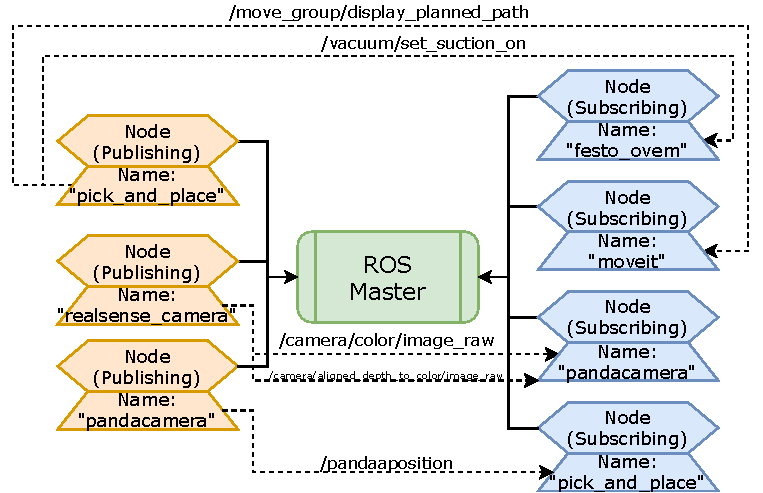
\includegraphics[width=0.8\textwidth]{graphics/ros.pdf}
 \caption{ROS setup}
 \label{fig:roswork}
\end{figure}

%The main hardware parts will be explained in several subsections: robot manipulator (\ref{subsec:robot}), robot end effector (\ref{subsec:robotend}) and a camera (\ref{subsec:camera}). 

\subsection{Data Annotation}
COCO Annotator is a web-based image annotation application that allows you to mark up images rapidly and conveniently to create training data for image localization and object detection\cite{brooks_jsbrokscoco-annotator_2021}. It has a variety of unique features, such as the ability to label an image segment, monitor object instances, label objects with disconnected visible sections, and store and export annotations in the well-known COCO format. An intuitive and customizable interface guides you through the annotation process, which includes a range of resources for constructing accurate datasets.
% \begin{figure}[h]
% \centering
% 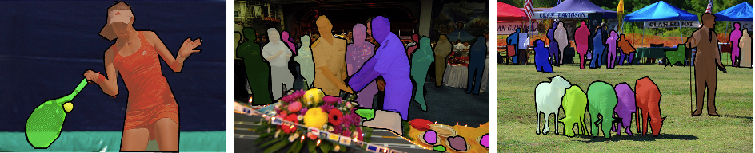
\includegraphics[width=1\textwidth]{graphics/coco.png}
% \caption{An example of how images are annotated by hand}
% \label{fig:coco}
% \end{figure}
% \linespread{0}

\subsection{Object detection}\label{sec:yolo}
You only look once (YOLO) is a real-time object detection system that is at the cutting edge of technology\cite{redmon_yolov3_2018}. 
It was first developed by Josep Redmon and is a convolutional neural network.
Object identification, classification, and localization are all performed in a single network pass with YOLO. 
As a result, it is more computationally efficient and robust than other networks that only perform one or two of these tasks at the same time. 
With the help of dimension clusters, YOLO predicts classes and bounding boxes (convolutional neural network). 
It's so computationally powerful that it can operate on a live image stream, which comes in handy when operating on a robot in real time.
\begin{figure} [ht]
 \centering
 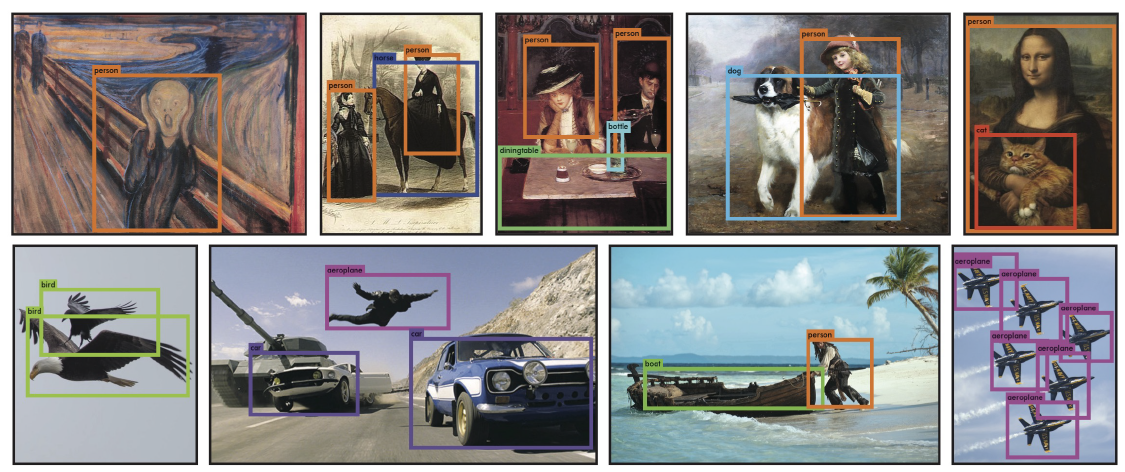
\includegraphics[width = 0.75 \textwidth]{graphics/yolo.PNG}
 \caption{You Only Look Once: Unified, Real-Time Object Detection \cite{redmon_you_2016}}
 \label{fig:yolo}
\end{figure}


In this project \textit{YOLOv4}\cite{bochkovskiy_yolov4_2020} algorithm was used to detect objects in the bin and mark a rectangle around them. 
YOLO algorithm was chosen since it is easy to use and the major advantage of YOLO is its excellent speed, it also understands the general representation of objects. YOLO algorithm outperforms other detection algorithms, including \textit{Deformable Parts Model(DPM)} and \textit{R-CNN}, when generalizing natural pictures from artworks to other fields\cite{zou_object_2019}.

%When the YOLO has found an object with high accuracy it sends to the robot coordinates of the center point, and then there is possible to get the depth from the camera.

% \begin{figure}[h]
% \centering
% 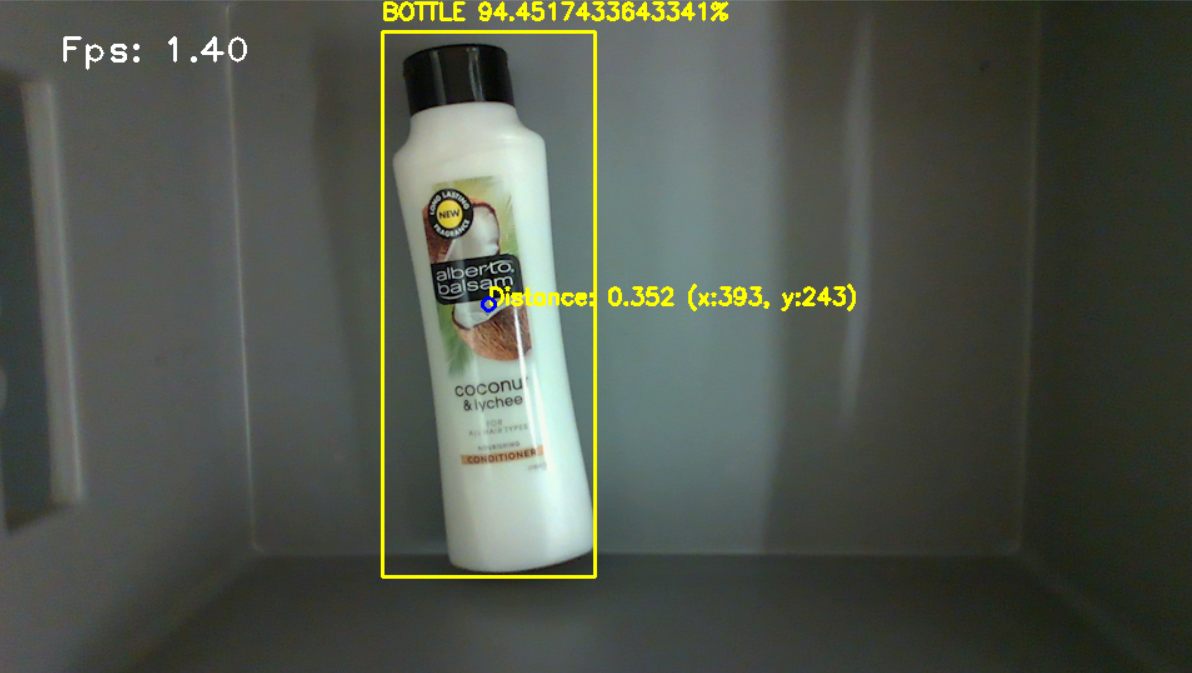
\includegraphics[width=0.4\textwidth]{graphics/detectandmeasure.PNG}
% \caption{Here is an example of an YOLO detect application}
% \label{fig:yolodetect}
% \end{figure}

\subsection{OpenCV}
OpenCV is a cross-platform library that allows one to build real-time computer vision applications. It is primarily concerned with image recognition, video capturing, and interpretation, with features such as face detection and object detection. OpenCV is a free and open-source library of programming functions primarily for real-time computer vision \cite{noauthor_opencv_nodate}.

One of OpenCV's aims is to provide an easy-to-use computer vision infrastructure that allows people to easily create fairly complex vision applications. Over 500 functions in the OpenCV library cover a wide range of vision applications, including factory product inspection, medical imaging, security, user interface, camera calibration, stereo vision, and robotics. Since computer vision and machine learning often go hand in hand, OpenCV includes a comprehensive, general-purpose Machine Learning library \cite{kaehler_what_2016}.

% \begin{figure}[h]
% \centering
% 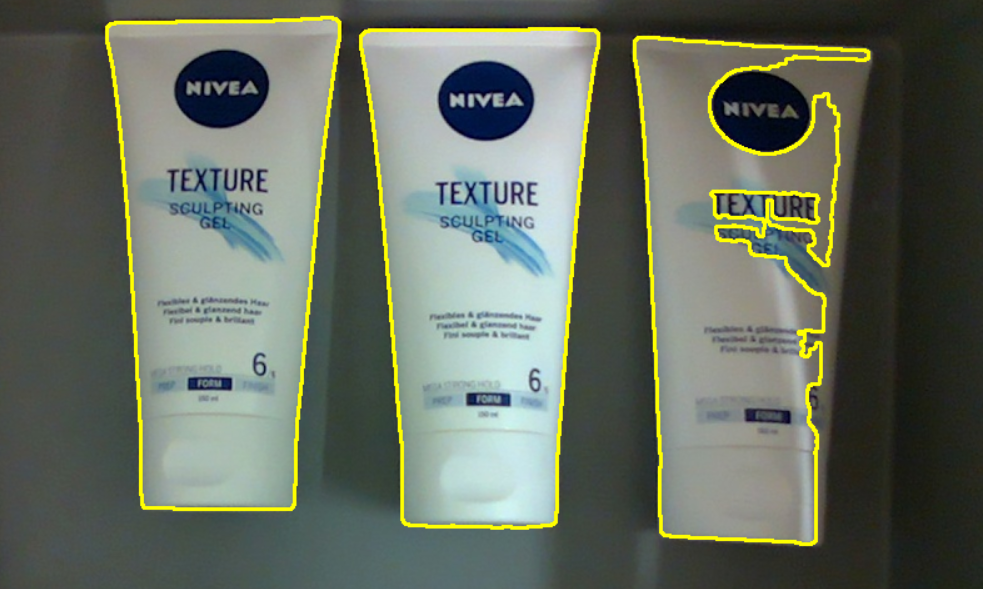
\includegraphics[width=0.65\textwidth]{graphics/contour.PNG}
% \caption{An example of how OpenCV can find contours}
% \label{fig:opencvcontour}
% \end{figure}

OpenCV was used in this project to work on images from the camera, the main functions that were used in this project were \textit{structural simularity} to compute the difference between two images, \textit{threshold} to threshold the difference image followed by finding contours to obtain the regions of the two input images that differ and then the \textit{findContours} function to find the contours, draw around the objects and measure the objects.
% breyta, say why I used each function and why opencv was used in that part....and so on44
% segja meira um hvern function t.d. structural simu og finna reference

\clearpage
\section{Hardware \label{sec:hardware}}
%\ifdraft{\textit{Hér skrifa ég hvað ég notaði og hvernig og referenca í undirkafla í hvert skipti (Má lesa yfir\\}}
This chapter includes a brief overview of the hardware that was used in this project. The main hardware parts will be explained in several subsections: robot manipulator \textit{(Sec:\ref{subsec:robot})}, robot end effector \textit{(Sec:\ref{subsec:robotend})} and a camera \textit{(Sec:\ref{subsec:camera})}. The setup can been seen in \textit{Figure \ref{fig:setupproject}}.

\begin{figure}[h]
 \centering
 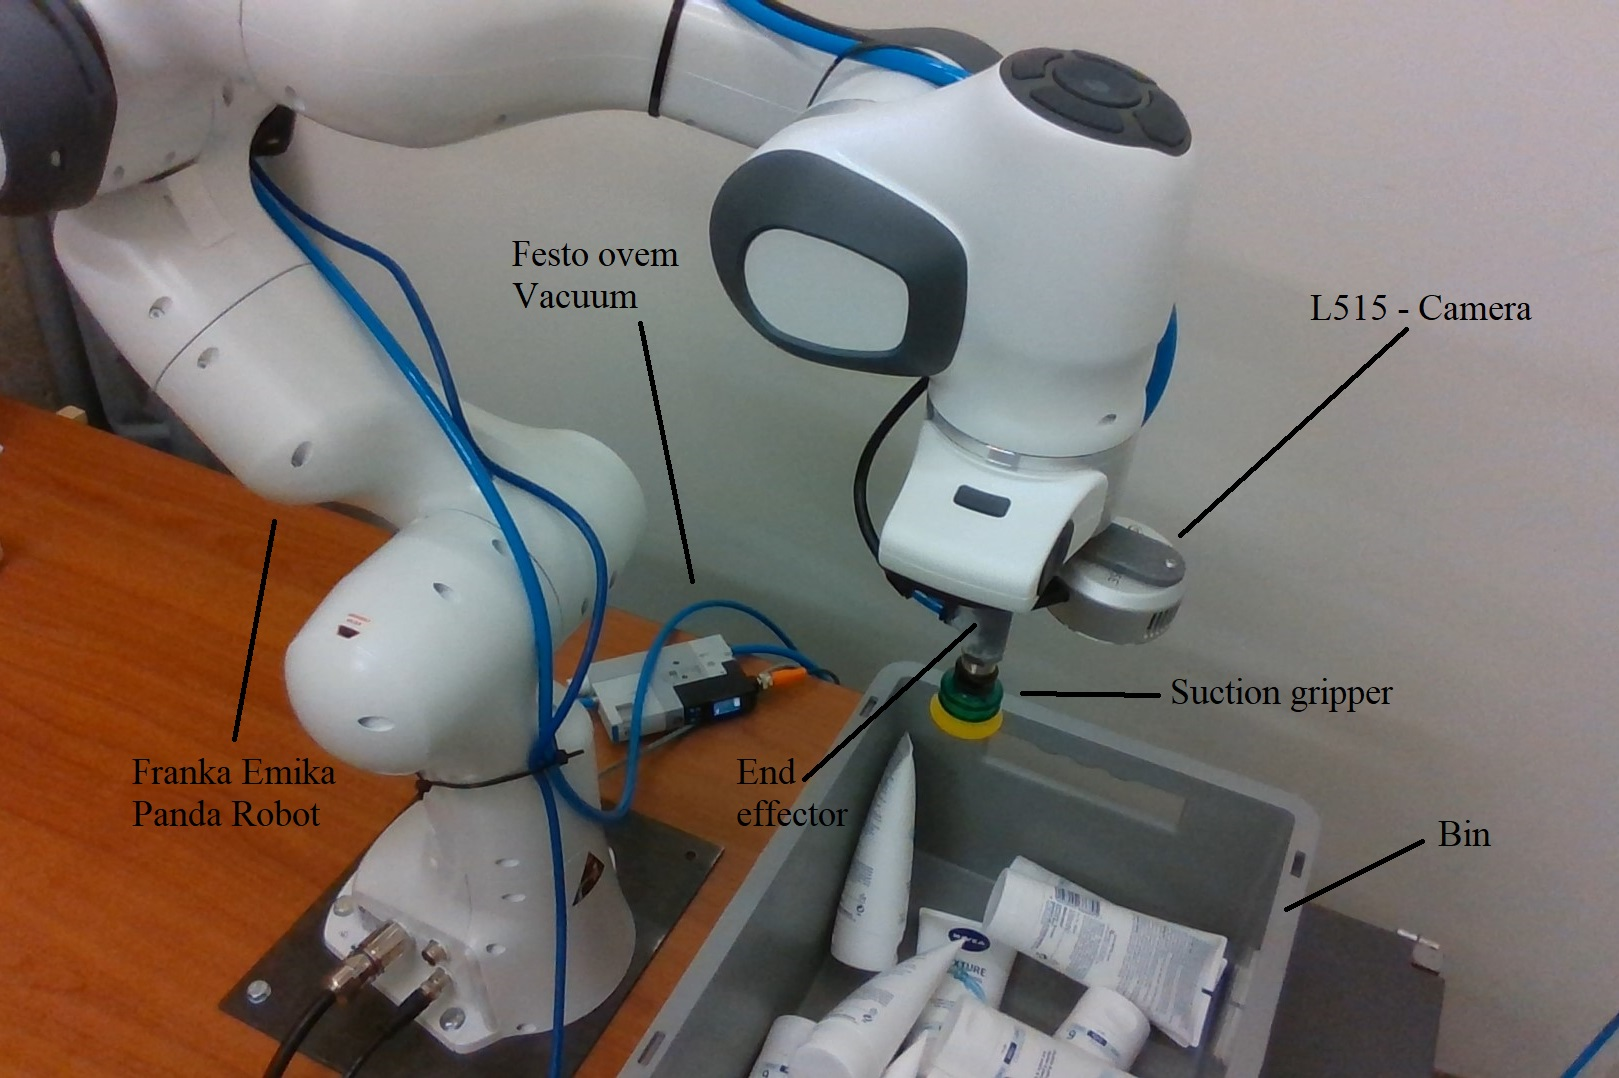
\includegraphics[width = 0.9\textwidth]{graphics/setup.jpg}
 \caption{The hardware setup for this project}
 \label{fig:setupproject}
\end{figure}
\linespread{0}
\subsection{PC cores}
\vspace{0.8cm}
\subsubsection*{Training neural networks}
The GPU for training neural networks will be the \textit{NVIDIA GeForce RTX 2080 Ti}\cite{noauthor_graphics_nodate}.
A GPU is nearly necessary to train neural networks. The GeForce RTX 2080 Ti is a budget-friendly option for the dense system configuration with a blower size. Titan RTX, Tesla V100, Titan V, GTX 1080 Ti, and Titan Xp provide the best price versus performance. Its performance at training neural networks is close to Tesla V100 speed, which is one of the world's most powerful GPU\cite{balaban_deep_2018}. 

\subsubsection*{Computer to control the robot}
The computer that will be used in this project to control the robot is a \textit{Lenovo ThinkCentre M83 SFF Pro Desktop}\cite{noauthor_thinkcentre_nodate} computer, it was chosen since it has ROS and had already been used to program the Franka Emika robot. 

\clearpage

\subsection{Robot manipulator\label{subsec:robot}}
The Robot manipulator that was used in this project is a Franka Emika Panda robot, a research robot located at the RU(Reykjavik University) Robot Interaction Lab. Franka Emika Panda is a Cobot that has 7 working axes with torque sensors in all 7 axes \cite{gmbh_franka_nodate}. Panda includes the characteristics of a conventional stiff industrial robot with a repeatability of +/- 0.1 mm even at elevated velocities of up to 2 m/s with a negligible direction variance. This enables accurate, resilient, and quick manufacturing method execution. 
% \begin{figure}[h]
% \centering
% 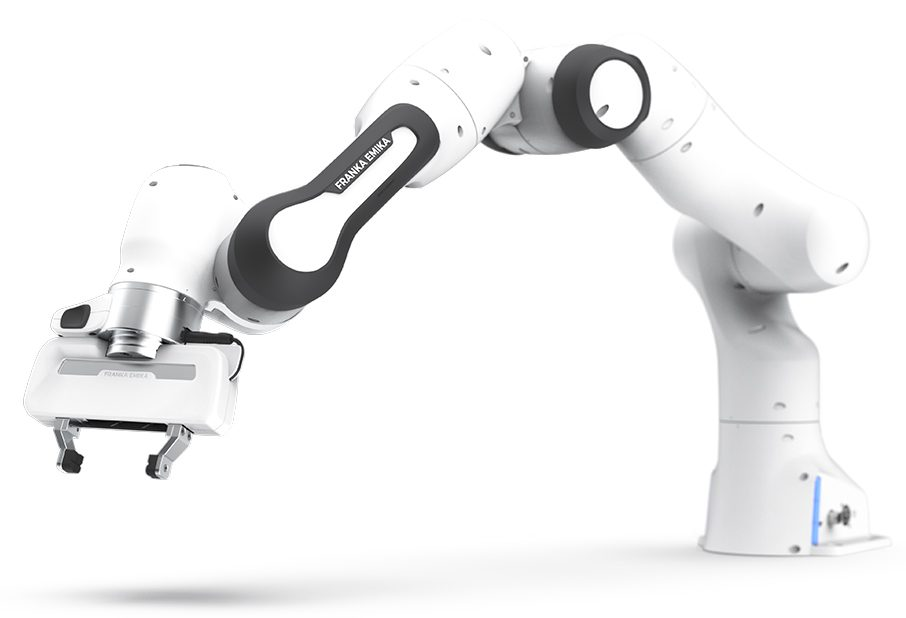
\includegraphics[width=0.8\textwidth]{graphics/frankapanda.jpg}
% \caption{Franka Emika Panda}
% \label{fig:frankaemika}
% \end{figure}
\begin{figure}[h]
 \centering
 % include first image
 \subfloat[Franka Emika Panda ]{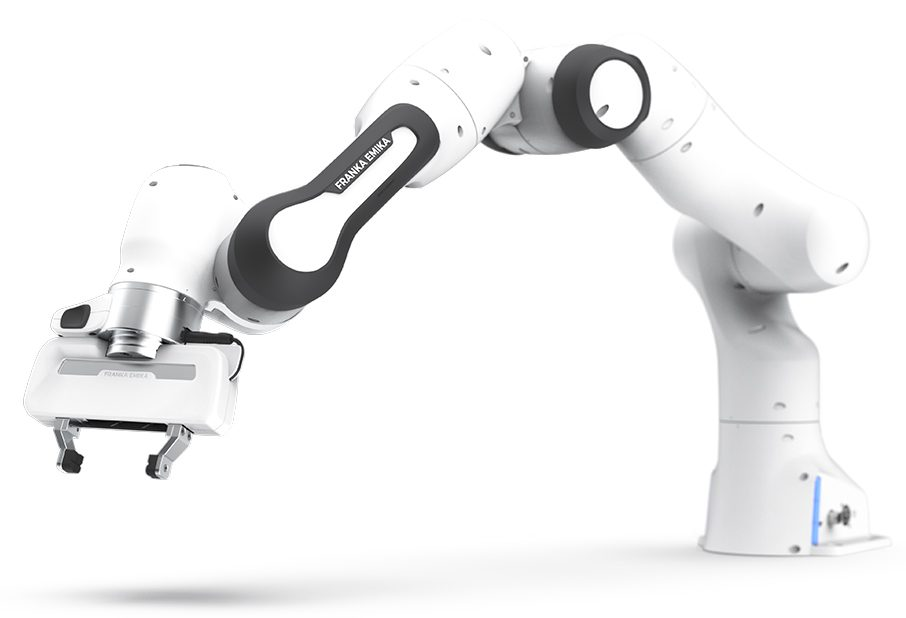
\includegraphics[width=0.5\textwidth]{graphics/frankapanda.jpg}}
 \hfill
 \subfloat[Franka Emika Panda setup]{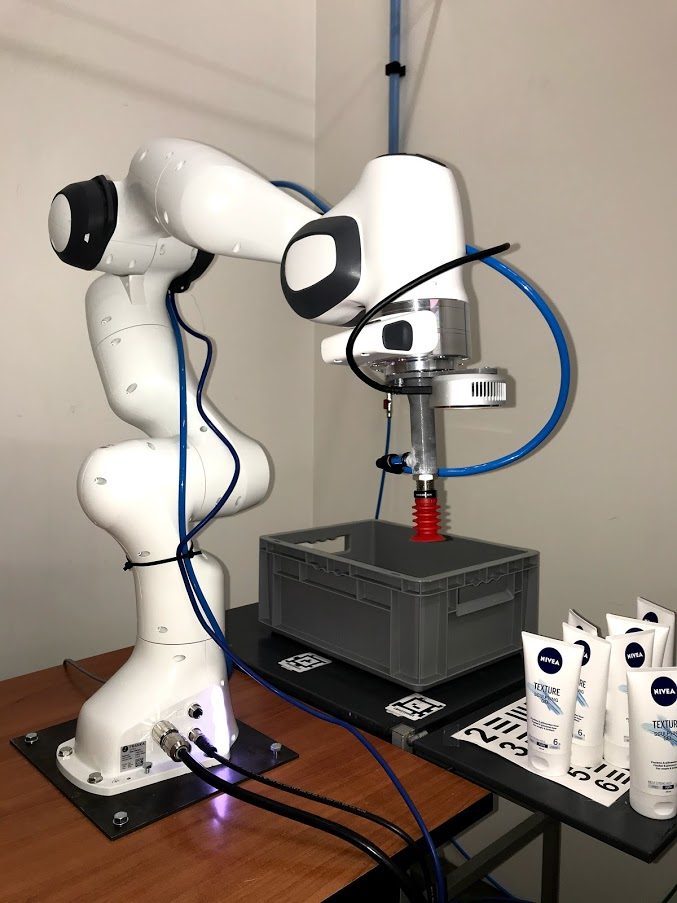
\includegraphics[width=0.3\textwidth]{graphics/pandarobot.jpg}}
 \caption{Robot manipulator}
 \label{figure: frankaemika}
\end{figure}
% Má eyða seinna\begin{itemize}
% \item \url{https://www.franka.de/}
% \item Franka Emika Panda in Gazebo with ROS and Docker \cite{wallkotter_franka_2020}
% \end{itemize}

\subsection{Robot end effector\label{subsec:robotend}}
A peripheral device that connects to a robot's wrist and allows it to communicate with its mission is known as an end effector. Grippers, process tools, and sensors are all examples of end effectors, which are mechanical or electromechanical \cite{wilson_relative_1996}. 

A suction gripper was designed and fabricated for use in the experiments, shown in \textit{Figure \ref{figure: endeffector}}.
It was designed in Autodesk Inventor \cite{noauthor_professional-grade_nodate} and 3D printed in TEVO Nereus 3D printer that Reykjavik University owns. At the end of the effector there is a suction cup connected to Festo Vacuum generator OVEM with an 8mm tube.
\begin{figure}[ht]
 \centering
 % include first image
 \subfloat[Inventor drawing]{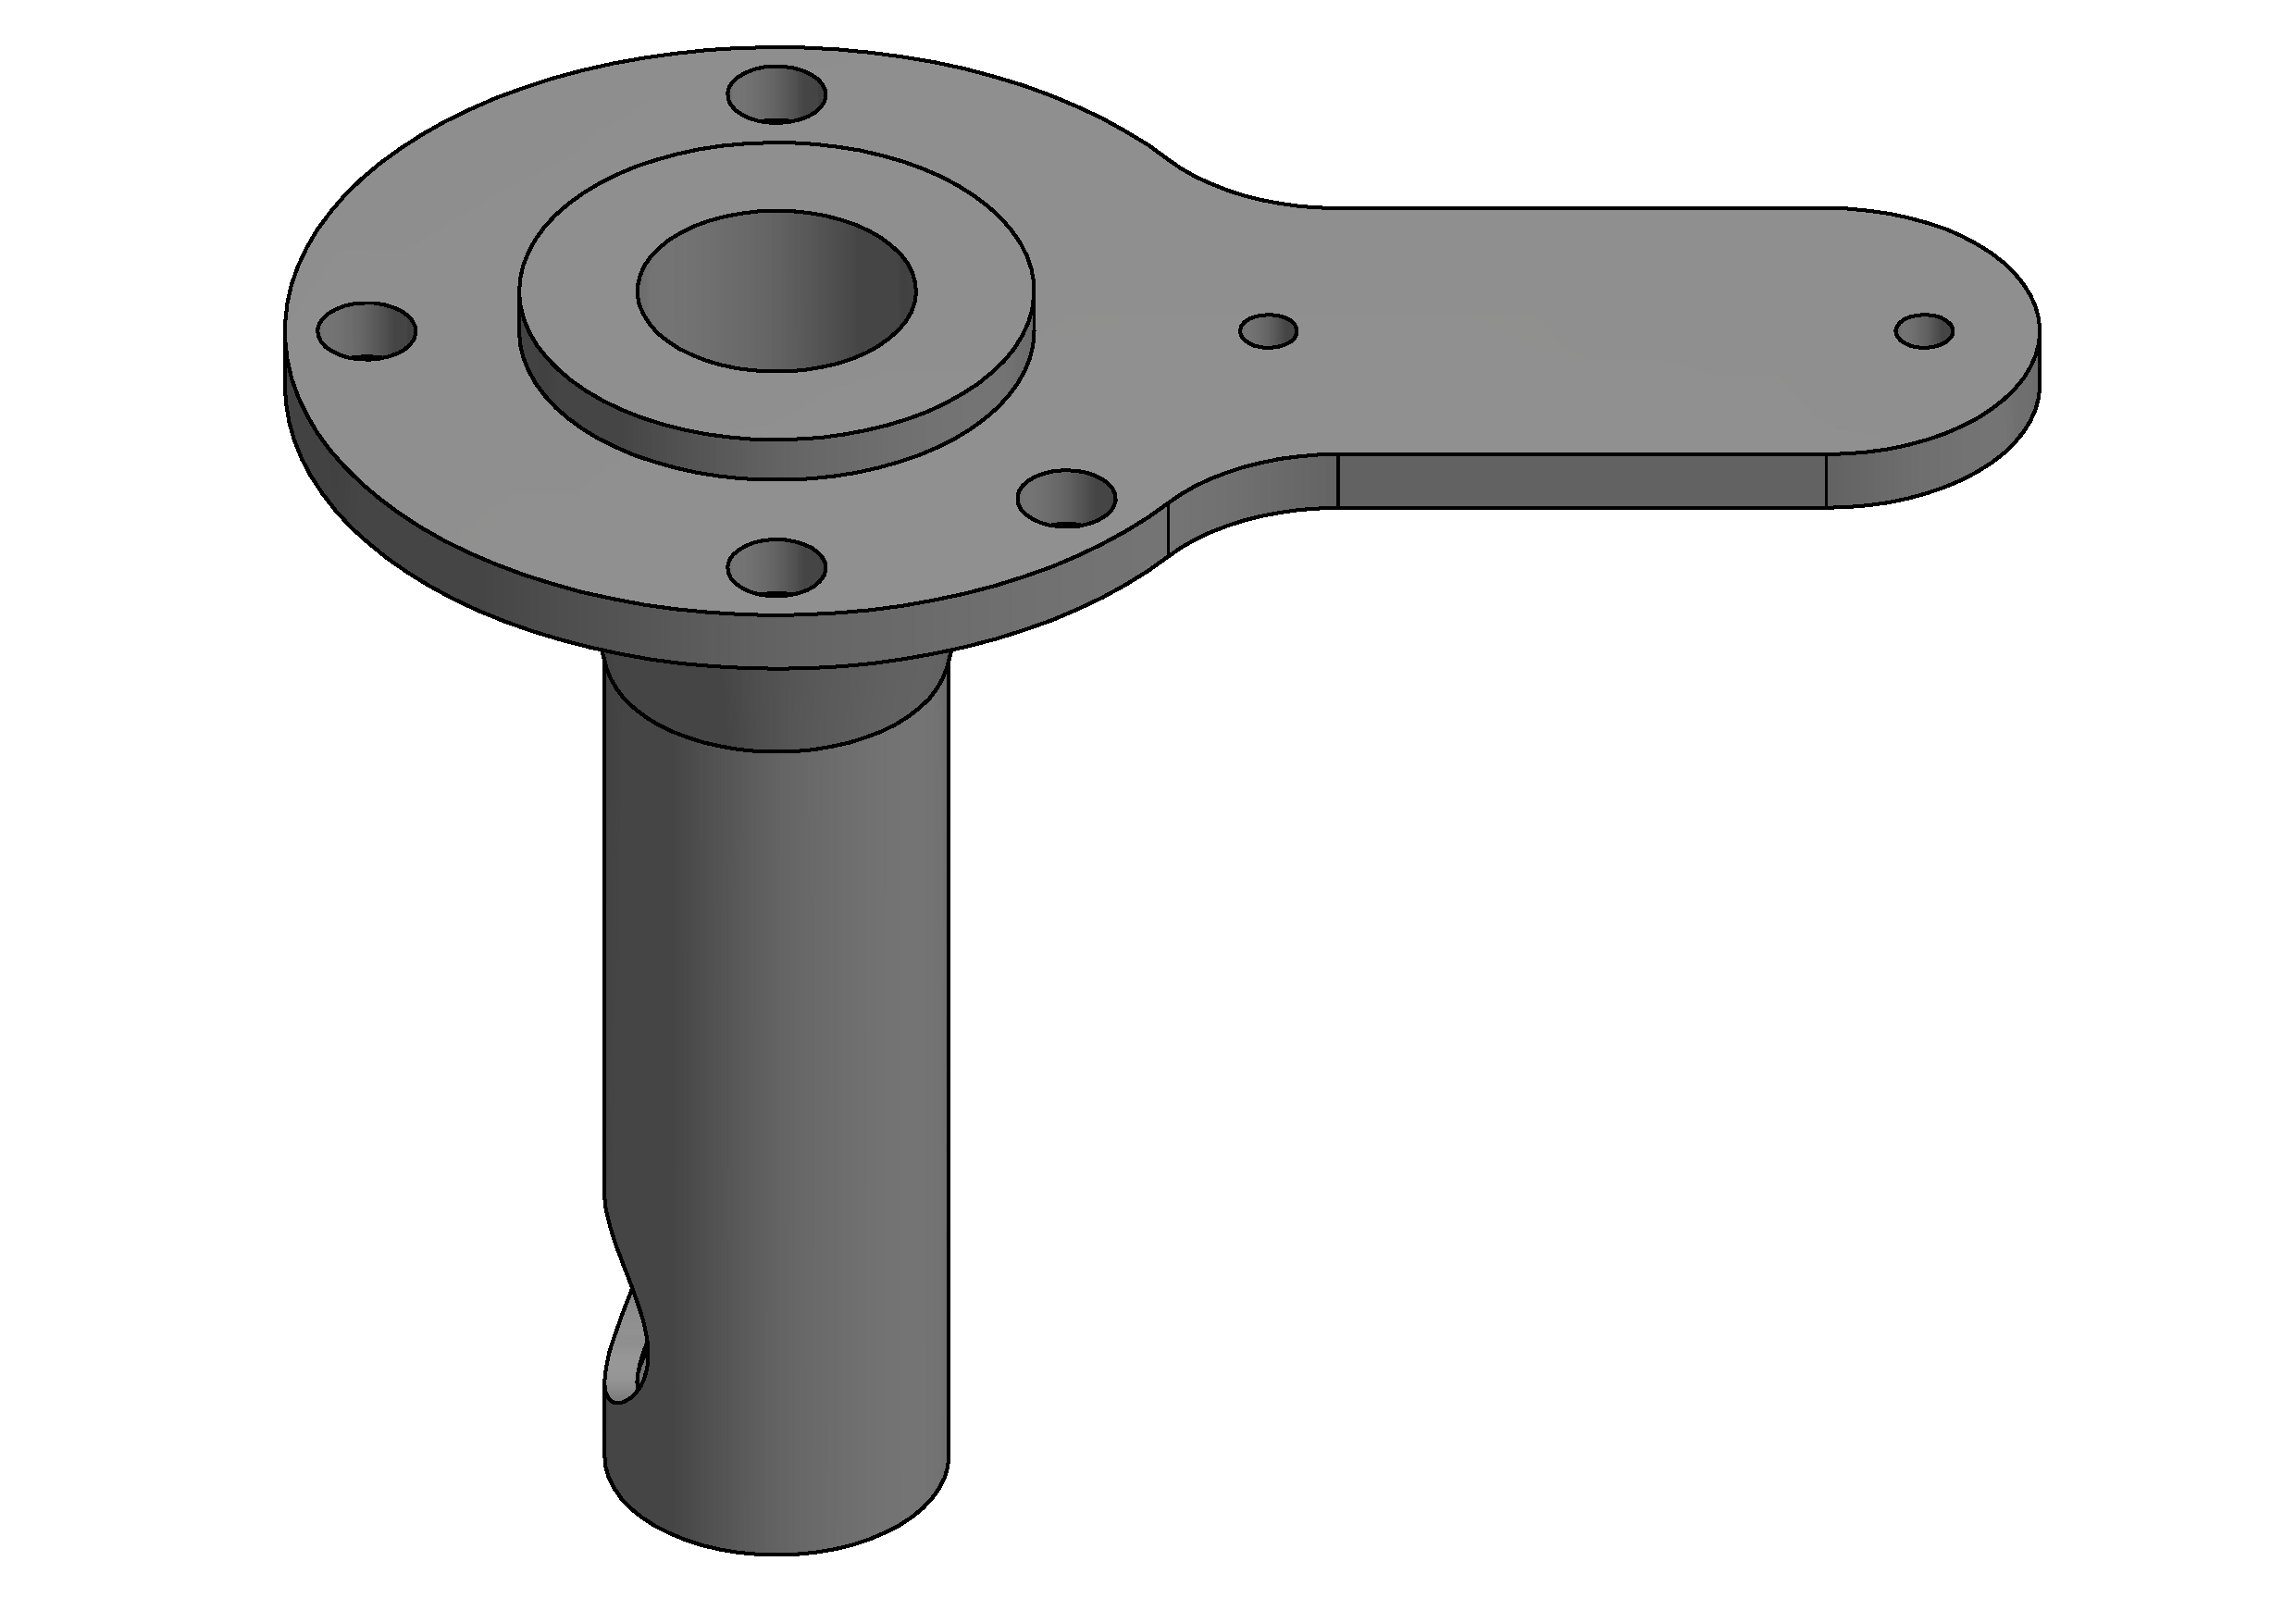
\includegraphics[width=0.33\textwidth]{graphics/single.pdf}}
 \hfill
 \subfloat[Completed end effector mounted on the robot]{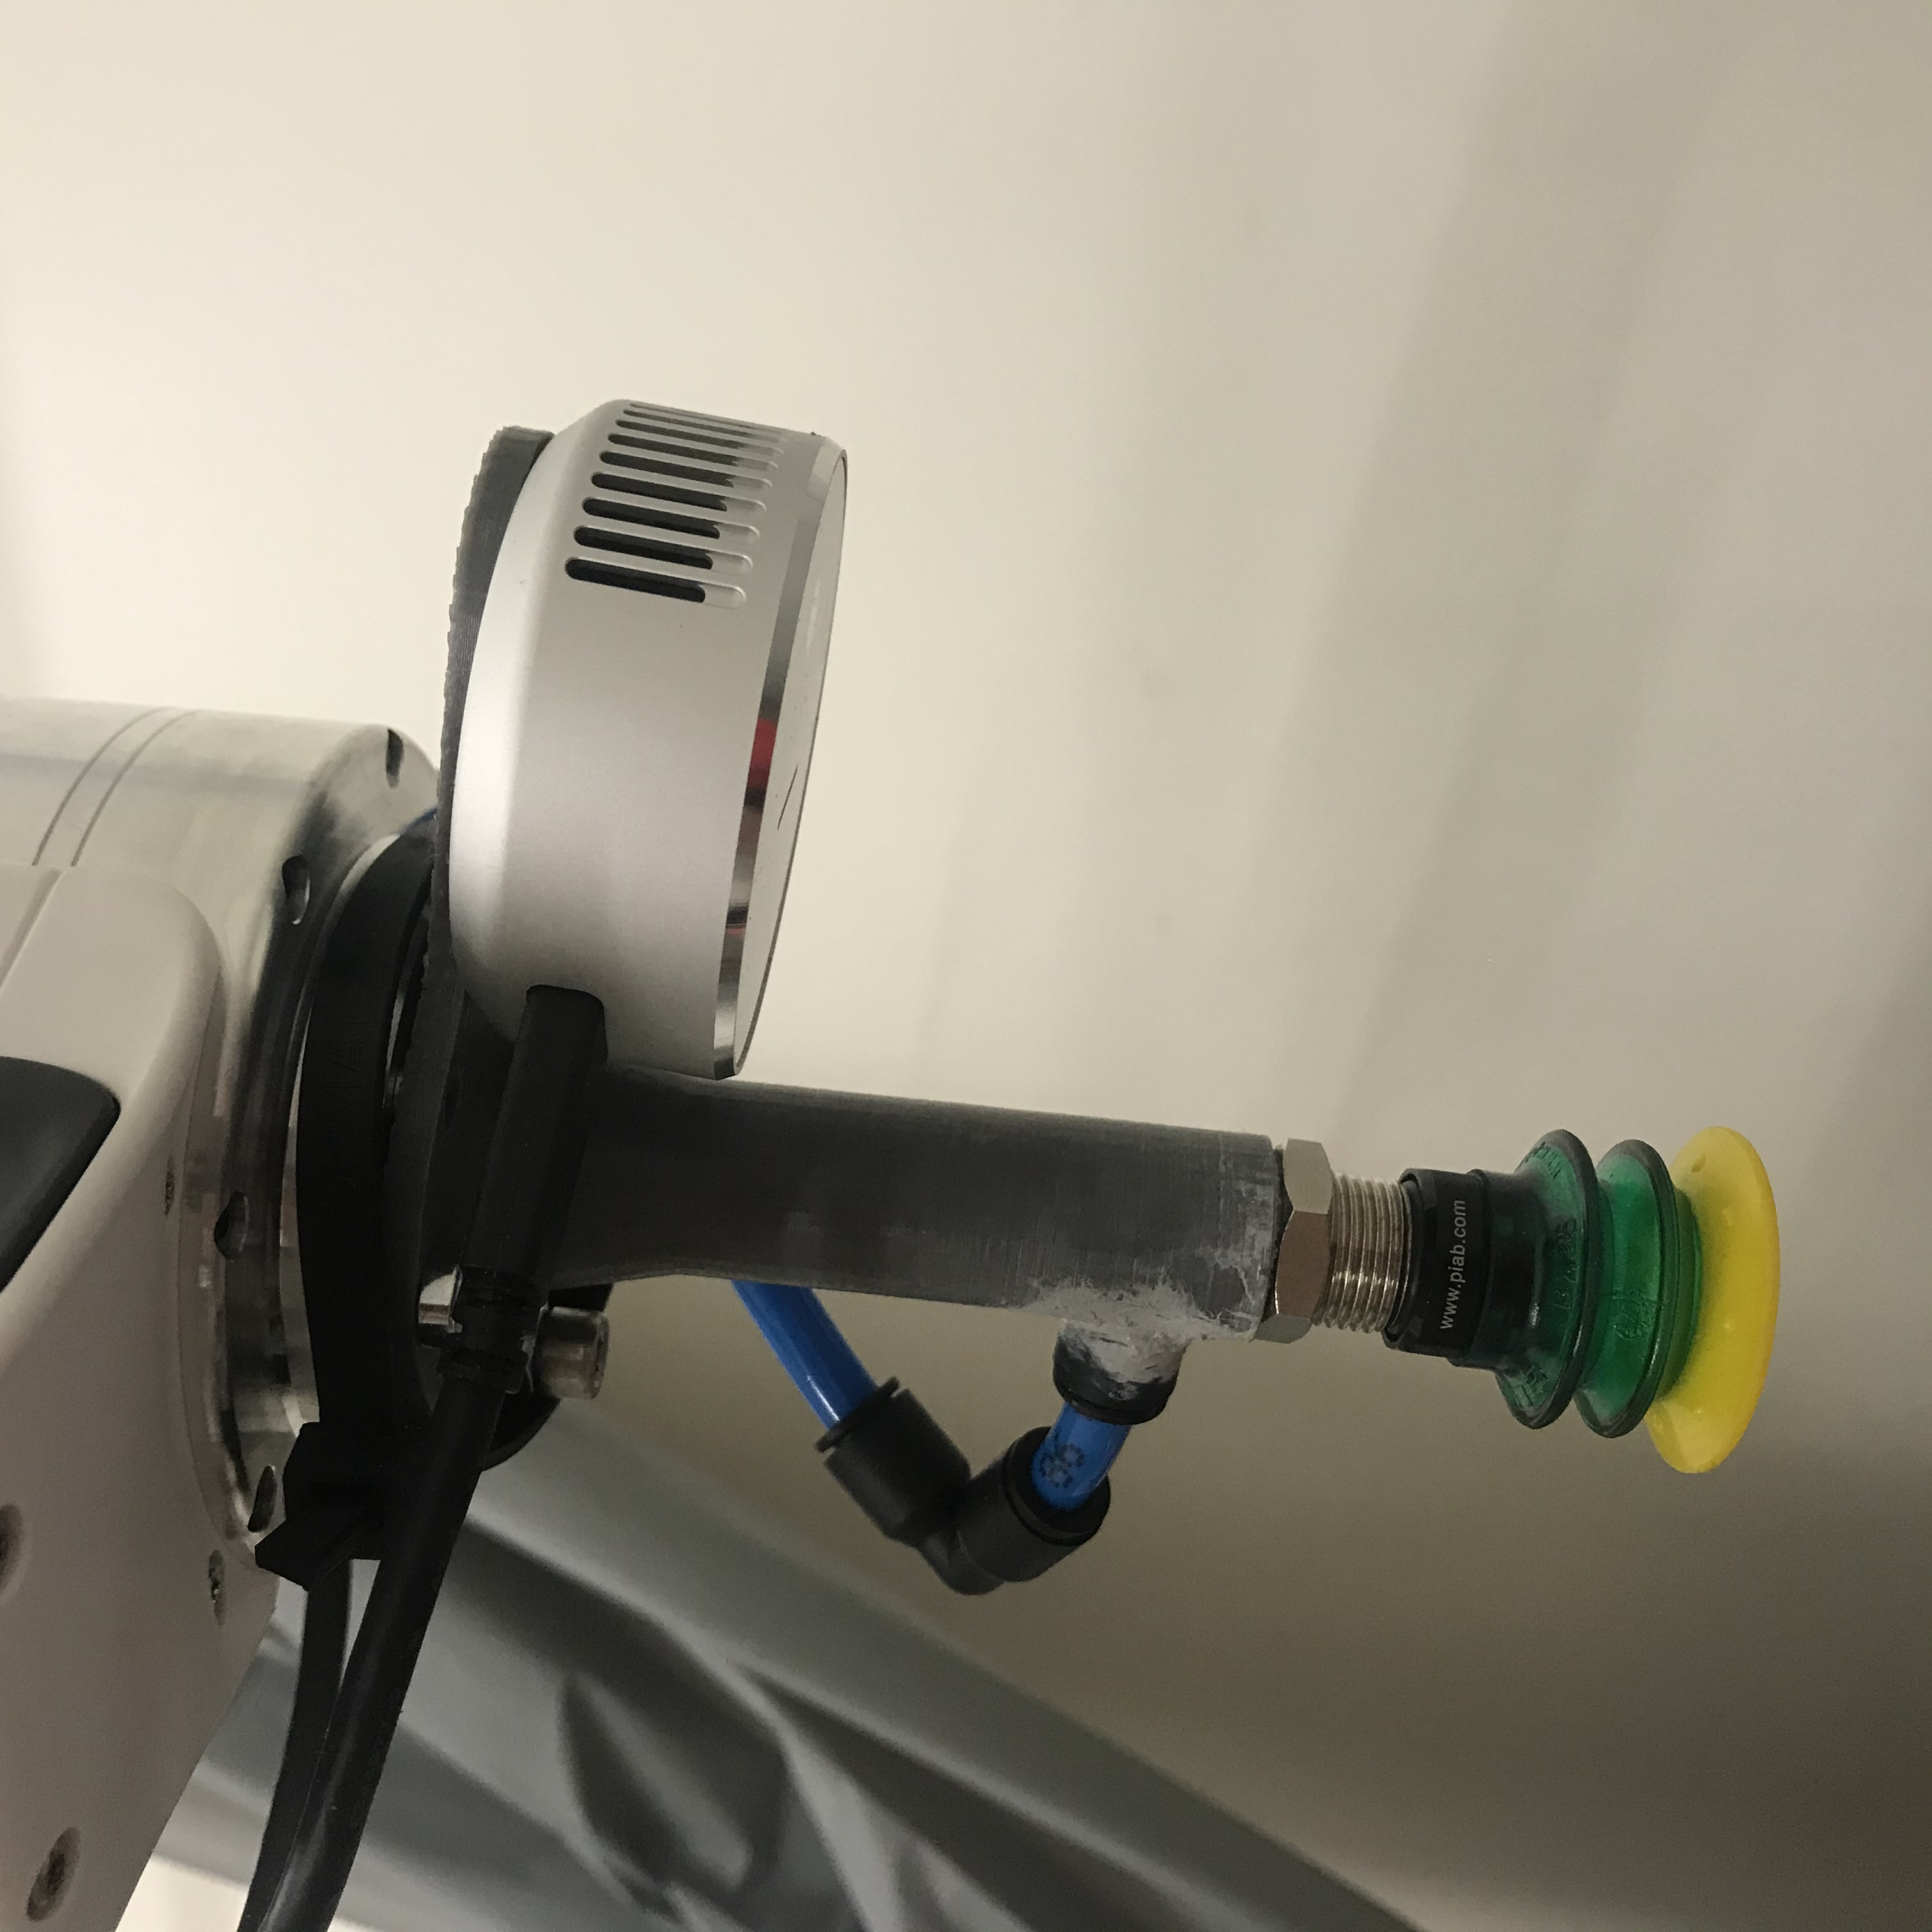
\includegraphics[width=0.27\textwidth]{graphics/methods/rani1.jpg}}
 \hfill
 \subfloat[The end effector extended by 14cm]{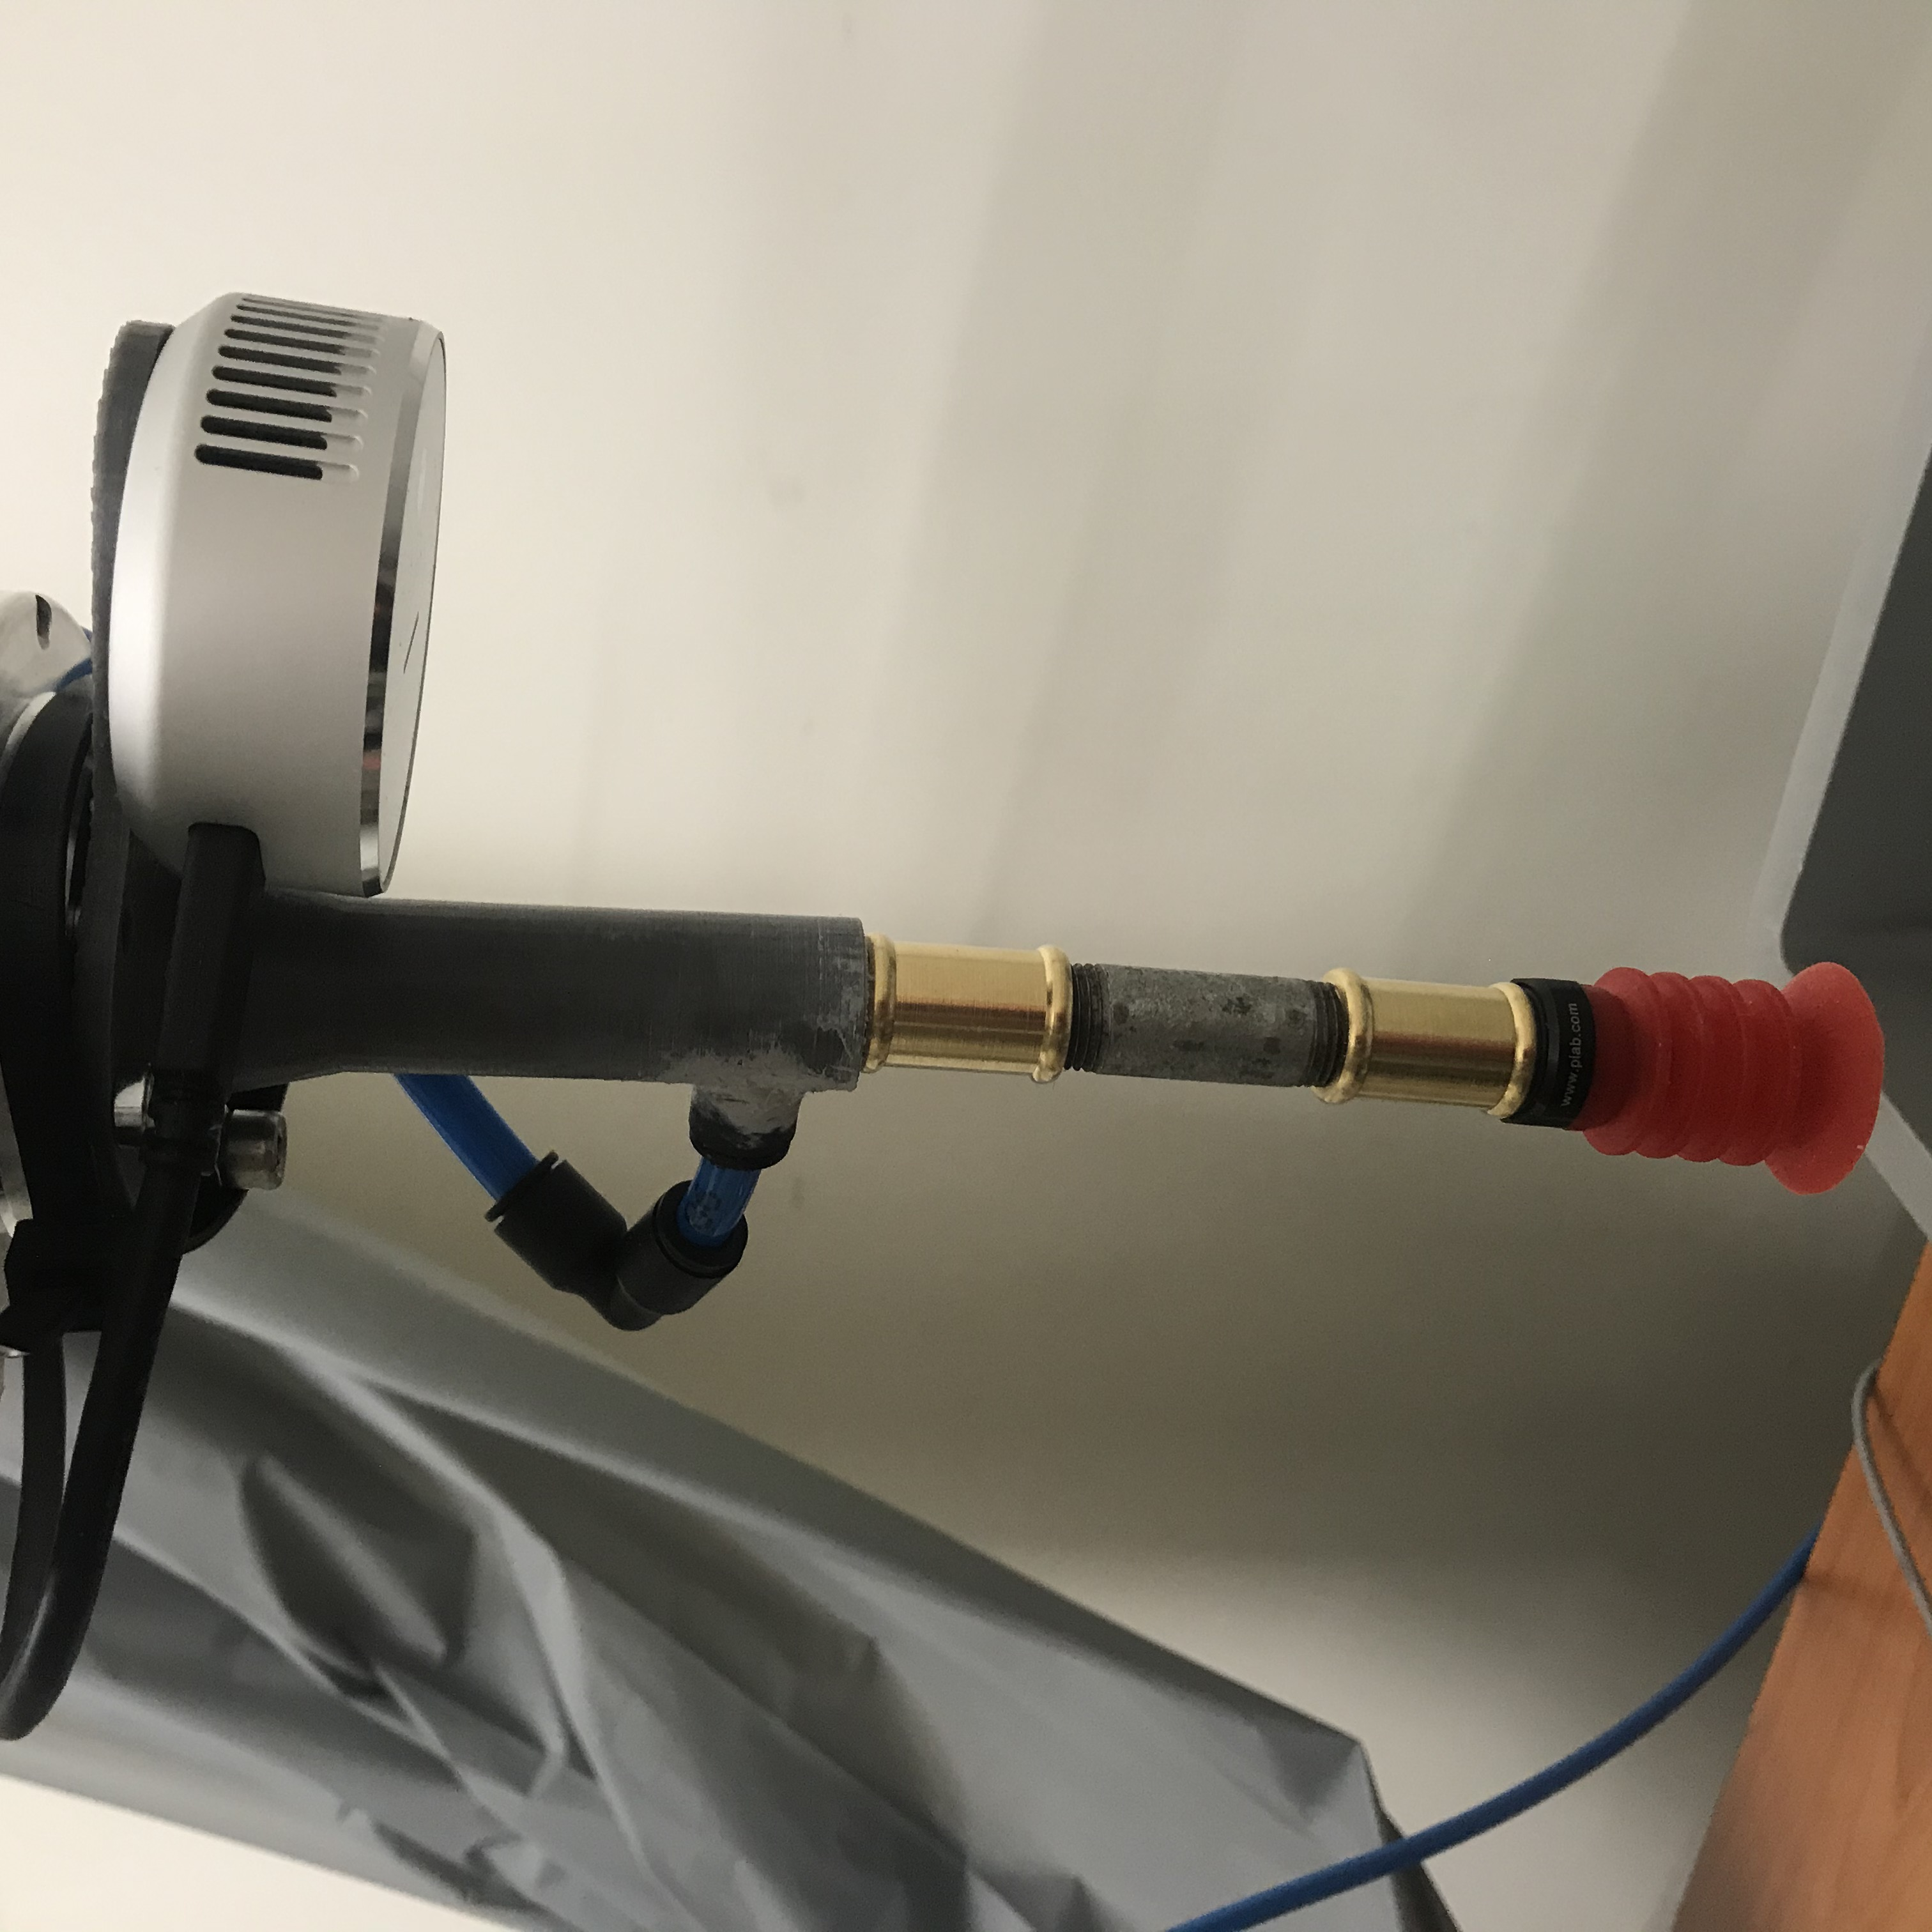
\includegraphics[width=0.27\textwidth]{graphics/methods/rani2.jpg}\label{figure: newendeffector}}
 \caption{Robot end effector}
 \label{figure: endeffector}
\end{figure}

\subsection{Camera\label{subsec:camera}} 
In this project, the Intel RealSense LiDAR Camera was used because it generates point clouds with depth information as well as color information from the embedded RGB cameras. LiDAR camera has the potential to provide a dense depth map even in homogeneous areas, where cameras based on passive stereo vision struggle to provide any measurement of depth. 
\begin{figure}[h]
 \centering
 % include first image
 \subfloat[RGB image]{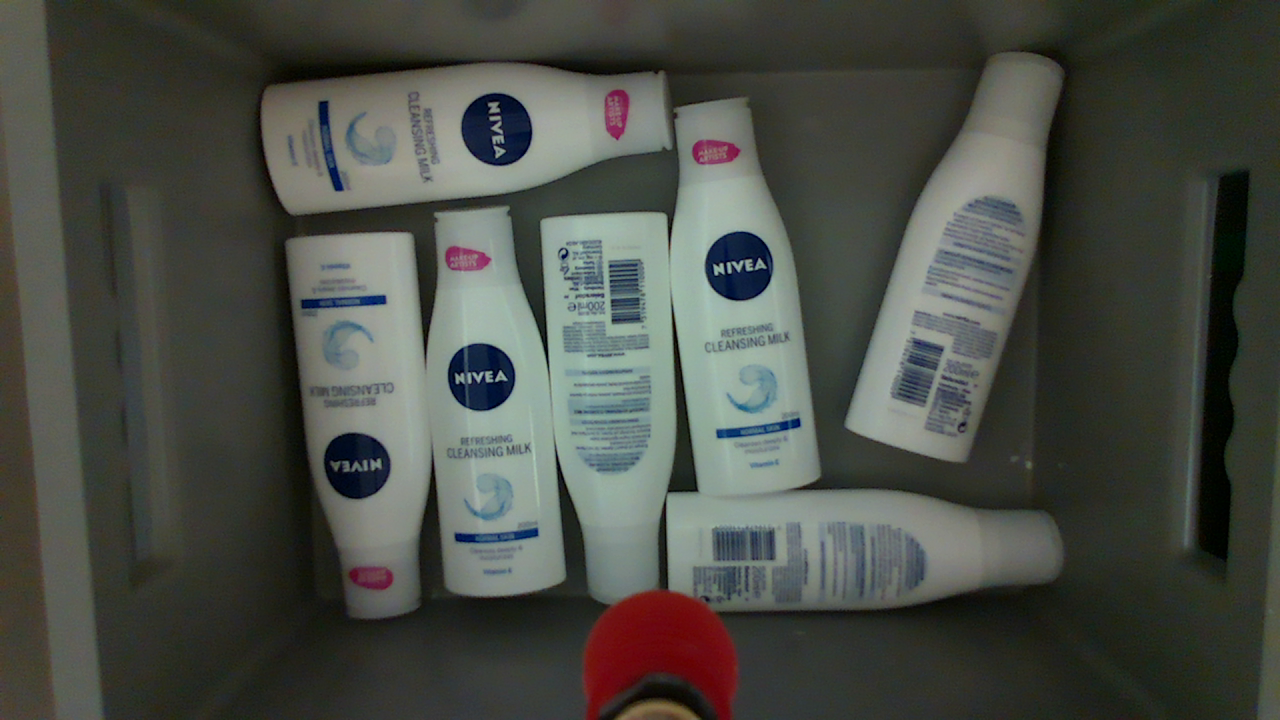
\includegraphics[width=0.47\textwidth,trim={4cm 0 4cm 0},clip]{graphics/methods/color_Color.png}\label{fig:l515depth}}
 \hfill
 \subfloat[Depth image]{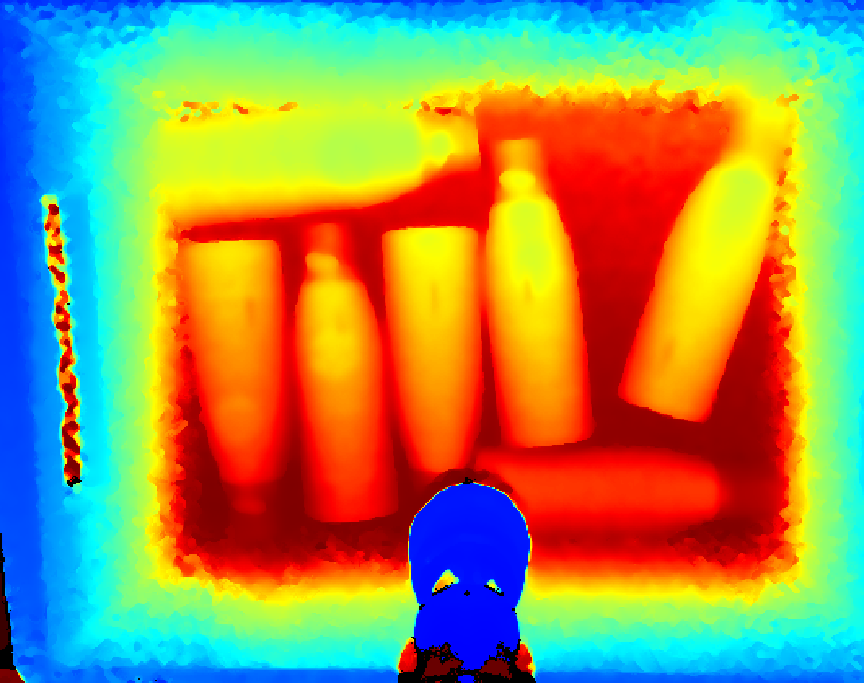
\includegraphics[width=0.42\textwidth]{graphics/methods/depth_Depth.png}\label{fig:l515color}}
 \hfill
 %\subfloat[The camera coordinates system]{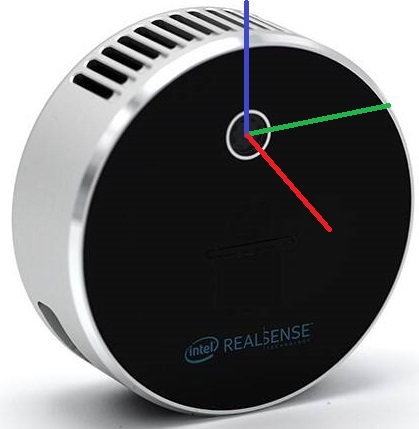
\includegraphics[width=0.27\textwidth]{graphics/lidar515.jpg}\label{fig:l515cor}}
 \caption{Example of output images from the L515 camera}
 \label{figure: lidar}
\end{figure}


The Intel RealSense LiDAR Camera makes use of a proprietary MEMS mirror scanning technology that increases laser power quality. The Intel RealSense LiDAR Camera has a high-resolution FHD RGB camera and an IMU for more reliable handheld scanning. With low power consumption and the ability to produce 23 million precise depth points per second, it's ideal for a wide range of applications. The LiDAR Camera L515 is designed for indoor use with adjustable lighting \cite{noauthor_intel_nodate}.


\begin{figure}[h]
 \centering
 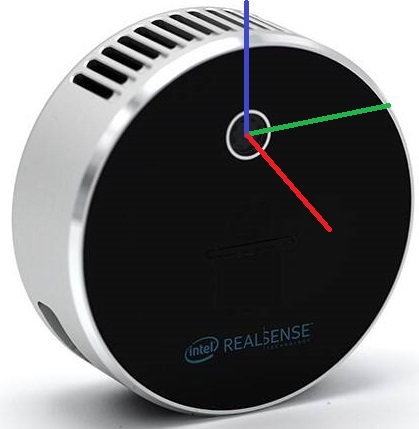
\includegraphics[width=0.5\textwidth]{graphics/lidar515.jpg}
 \caption{The camera coordinates system\cite{noauthor_intel_nodate}}
 \label{fig:l515cor}
\end{figure}
\clearpage

\section{Software implemented for experiments}
%% \
%\fxfatal{Start by stating what the implemented software is supposed to do and connect this to the objectives. Then proceed to describe how the software is divided into three components and describe each one in broad terms.}
The software implemented for the project experiments were three codes and one launch file and were created to answer the research questions\textit{(Appendix: \ref{app:code})}. There were implemented two software modules(\textit{pick\_and\_place and find\_pickpoint}) to generate new arrangements of objects using a robot manipulator, and one code to annotate objects automatically, determining the extent of the objects in the images(\textit{difference)}.

The panda\_bringup was used to launch the robot, camera, the suction, and the motion planner\textit{(Appendix:\ref{sec:pandabringup})}. 
The pick\_and\_place code controls the robot \textit{(Sec:\ref{sec:robot})}, 
find\_pickpoint talks to the camera and uses data to locate items \textit{(Sec:\ref{camera})} and then the difference which finds the difference between before and after picture and labels the images \textit{(Sec:\ref{labelimg})}.


\begin{figure}[h]
 \centering
 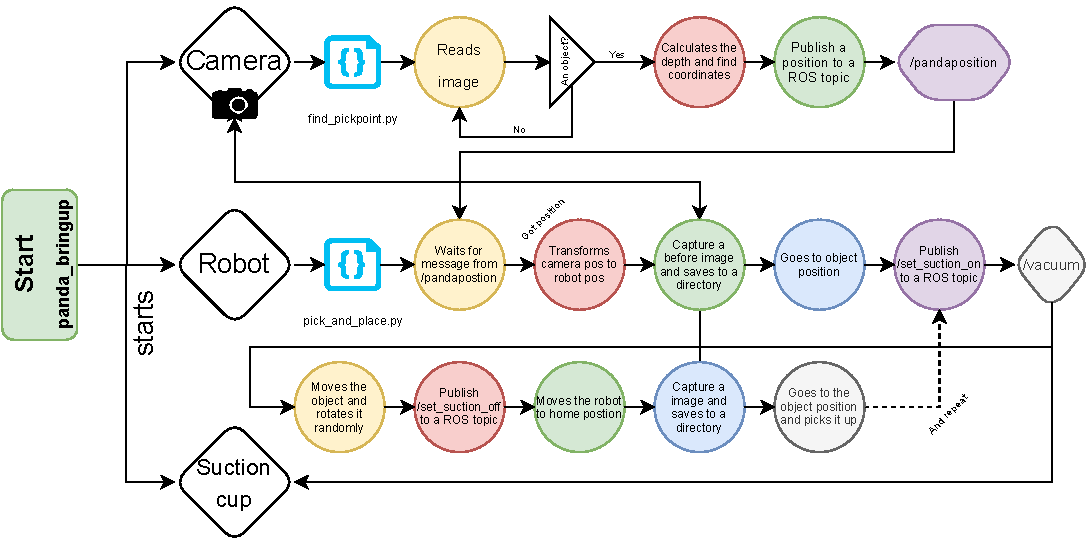
\includegraphics[width=1\textwidth]{graphics/softwareDiagram.pdf}
 \caption{Software diagram that shows how the panda\_bringup works}
 \label{fig:softwarediagram}
\end{figure}
The software diagram in \textit{Figure \ref{fig:softwarediagram}} shows the interaction between the hardware and the software modules. The camera reads images and calculates the depth, the robot picks the object at the desired position and moves it to another position and the suction cup takes commands from the robot.

\subsection{Automatic generation of training images}\label{sec:robot}
Two versions of the software were created to control the robot. One that only moved one object around inside of the bin and captured images, this version was used when the bin had a single object in the bin. The second version picked up one object and moved that object to another bin, this version was used when the bin had multiple objects in the bin.

The robot manipulator was programmed in python and used ROS to communicate with the robot, the two versions of the software can be found in the \textit{Appendix \ref{sec:pickandplace}} and \textit{Appendix \ref{sec:v2pickandplace}}, known as \textit{pick\_and\_place.py} and \textit{v2pick\_and\_place.py}. 
Both versions of the software, start by creating two ROS publishers, one that talks to the Festo vacuum suction cup and the other that talks to the MoveIt! motion planner. 
It also to creates a TF(transform) listener so it is possible to read the current positions and orientations, also it can transform poses between the coordinate frames attached to each link of the robot. The robot coordinates system is explained in \textit{Figure \ref{fig:pandachain}} 

\subsubsection{Training images with single object in the bin}\label{robotcontrol}
This is the first version of the software, and it moves one object inside of the bin. The software has a loop that runs while ROS is running. 
Where the robot waits for a message from the find\_pickpoint.py through a ROS topic where it gets an object position from the camera.
The TF listener then transforms the object position in camera coordinates to world coordinates. The robots then move to the object position and pick up the object using the suction cup. When the robot has picked up the object successfully it moves the object to another position and rotates the object by a random amount. When the robot has successfully moved the object it goes to the fixed home position and takes an image and saves it into a directory. 

\begin{figure}[h]
 \centering
 % include first image
 \subfloat[Starts in home position and capture an image]{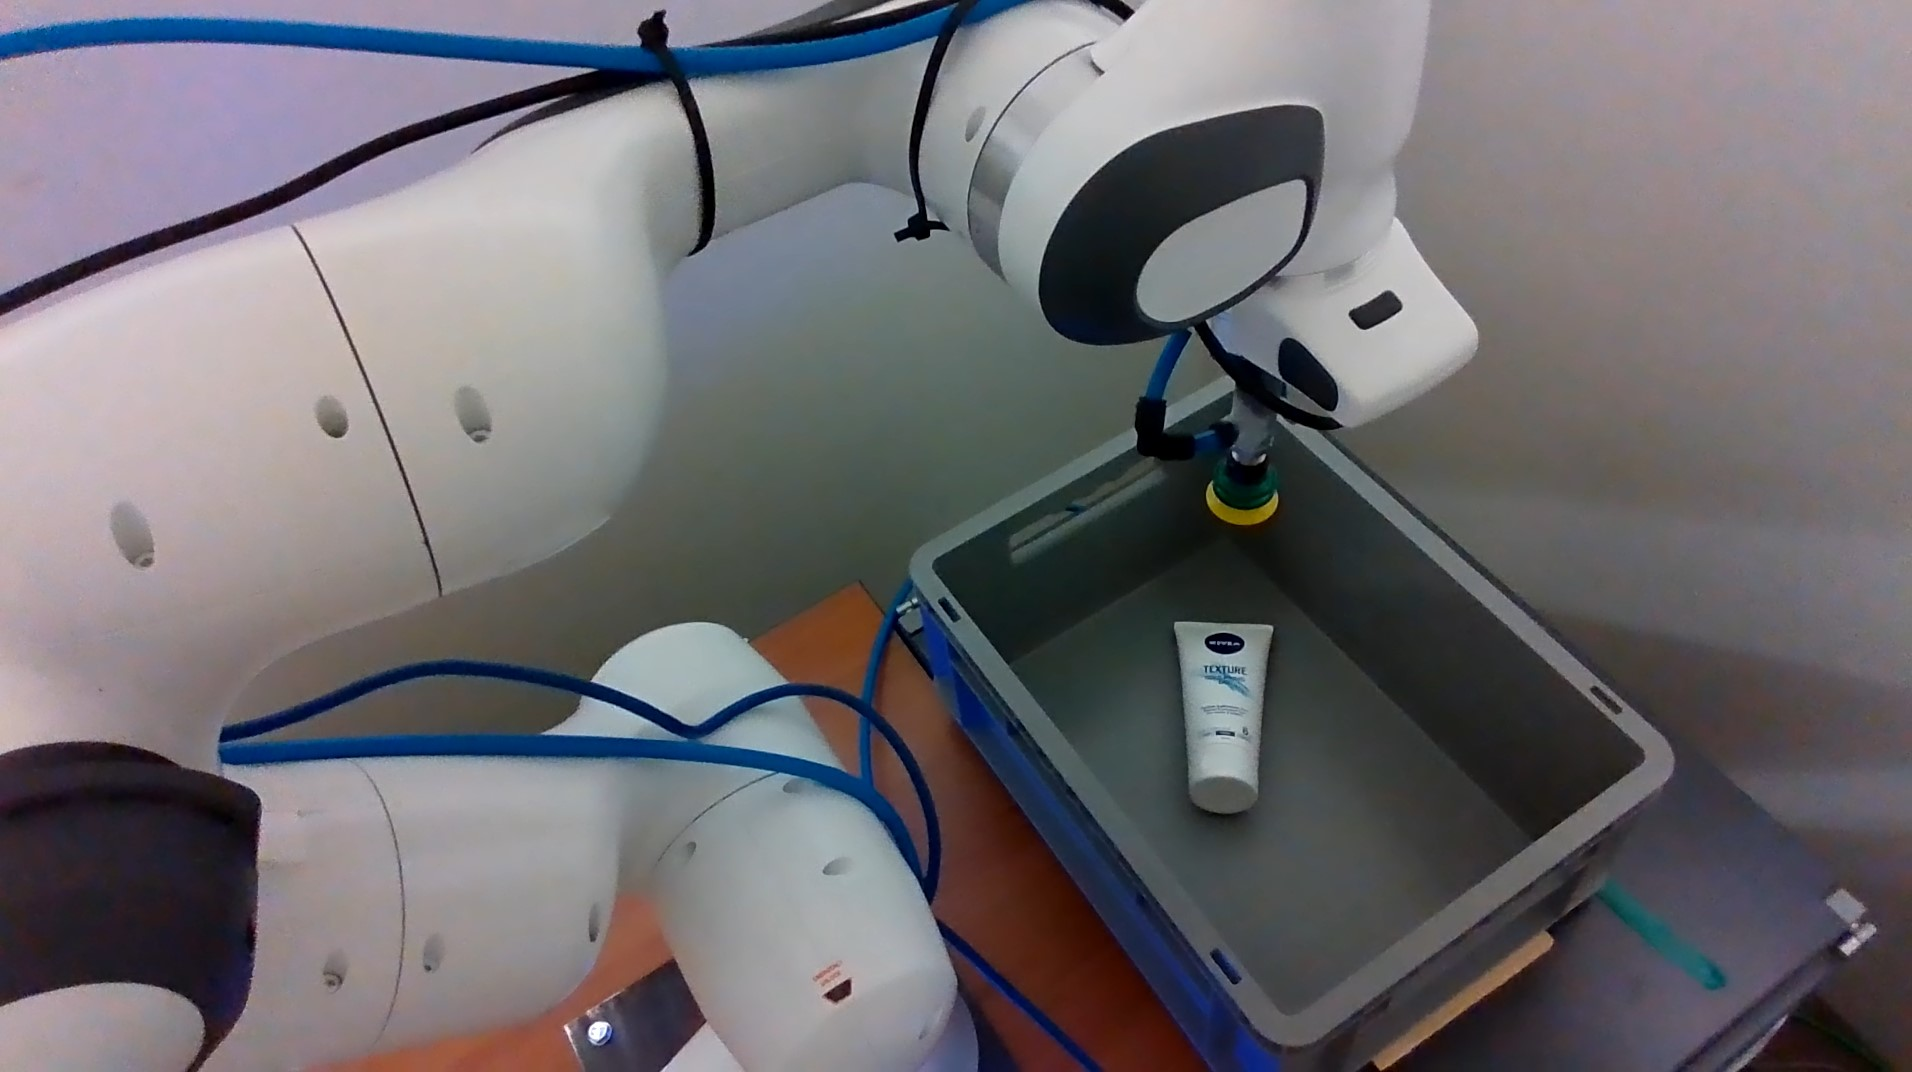
\includegraphics[width=0.3\textwidth]{graphics/results/1home.jpg}}
 \hfill
 \subfloat[Goes to the object]{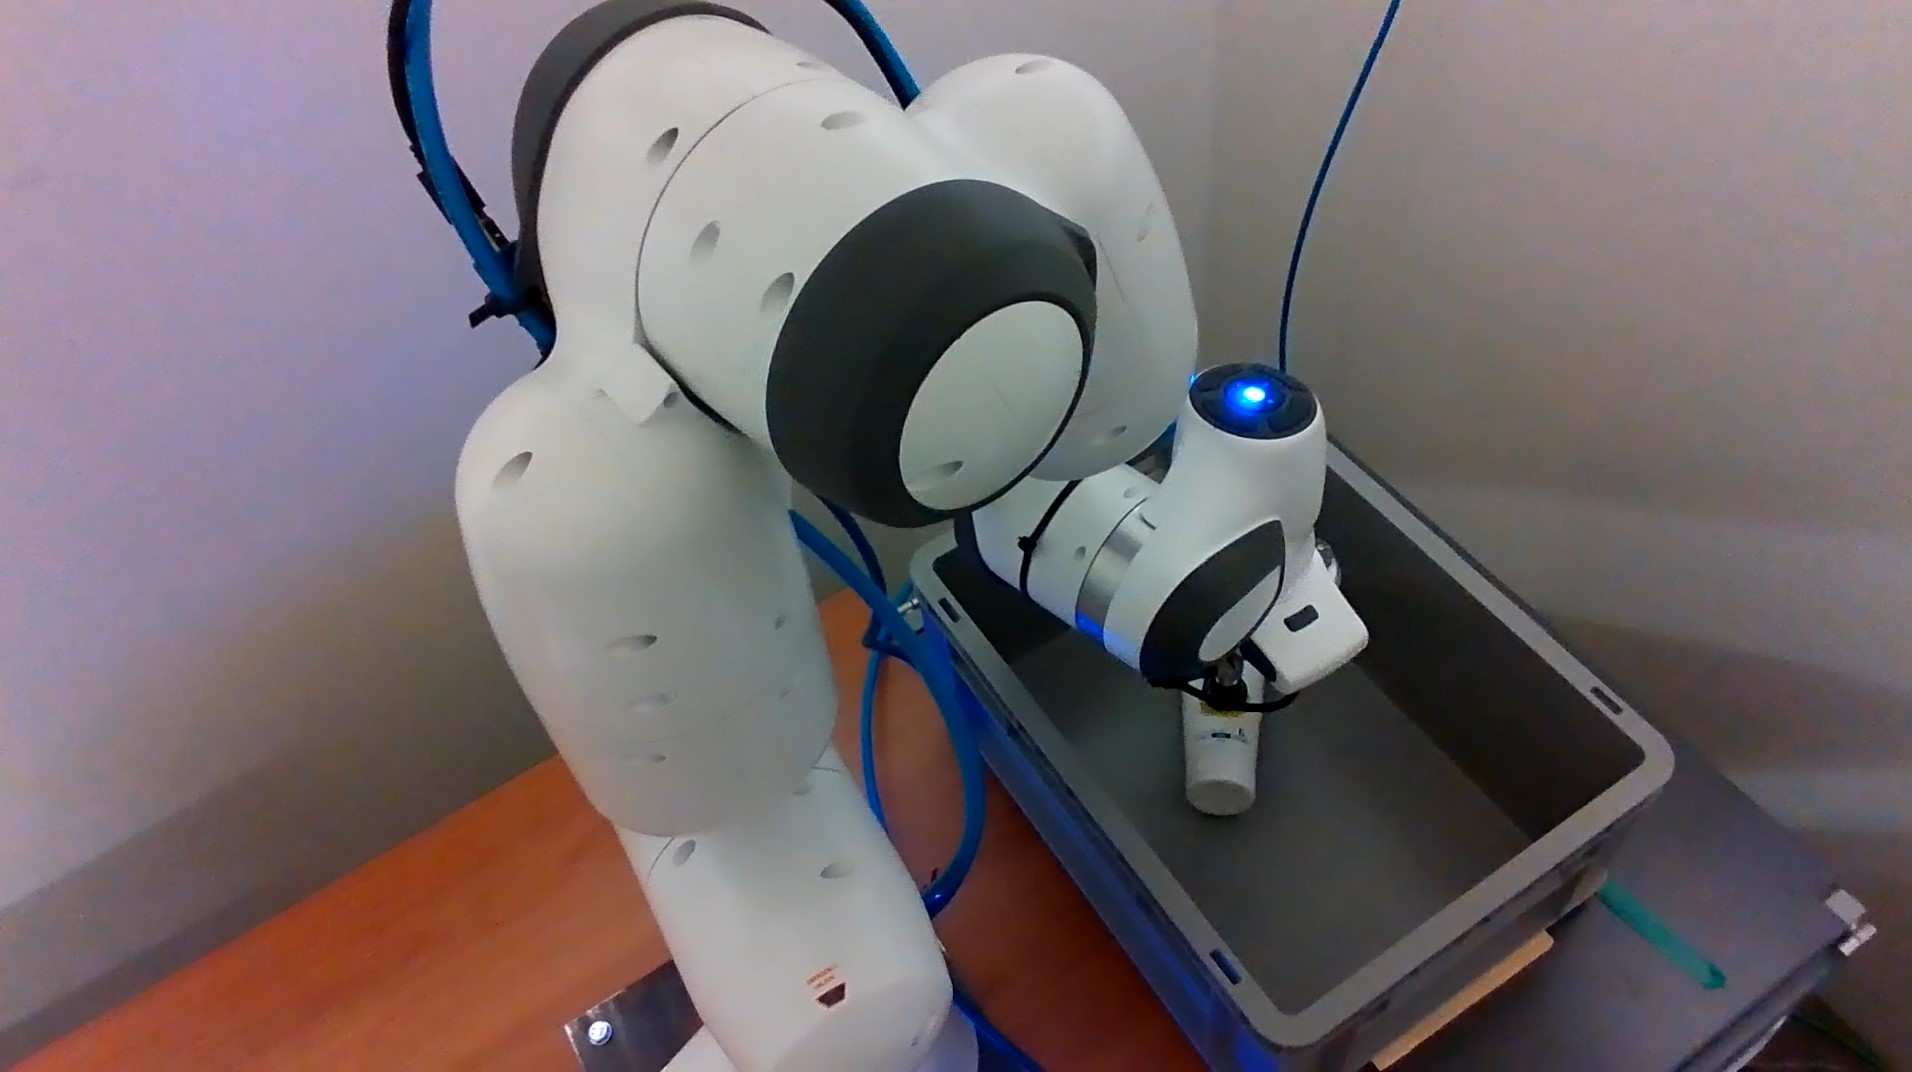
\includegraphics[width=0.3\textwidth]{graphics/results/2pick.jpg}}
 \hfill
 \subfloat[Picks up the object]{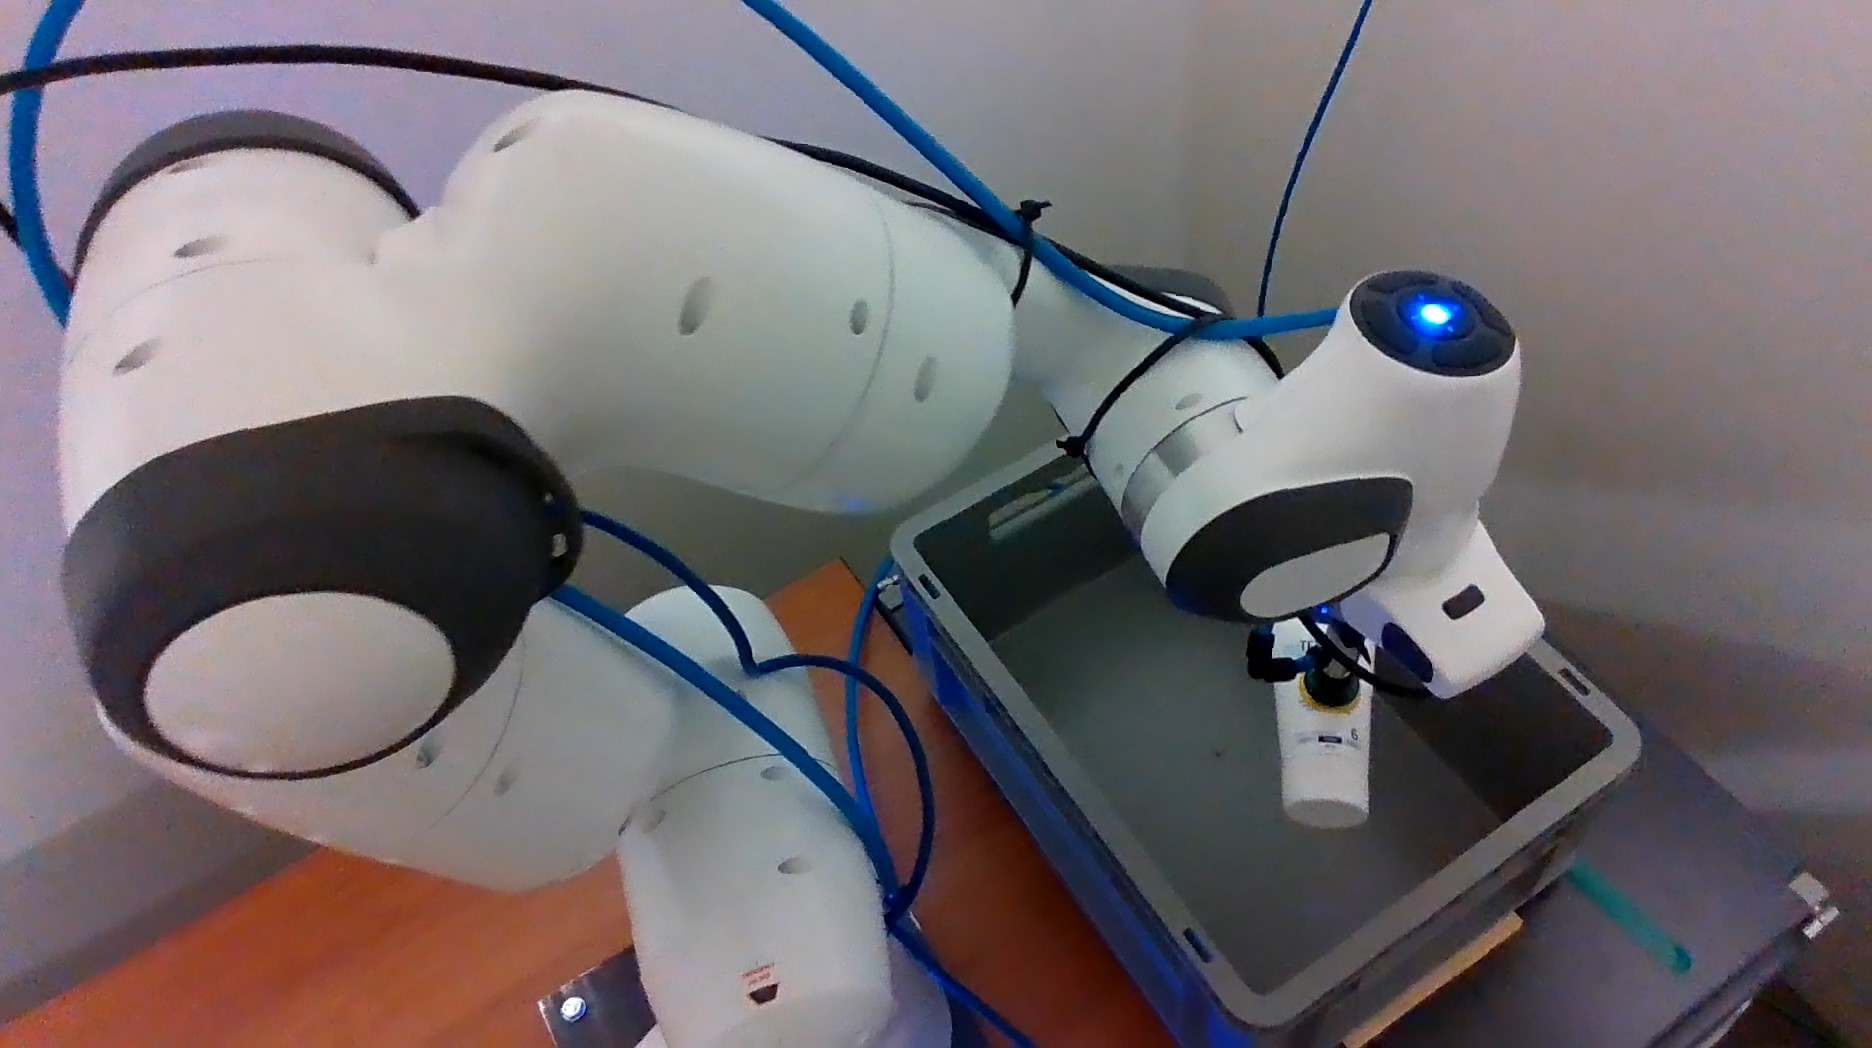
\includegraphics[width=0.3\textwidth]{graphics/results/3move.jpg}}
 \hfill
 \subfloat[Moves the object to another position]{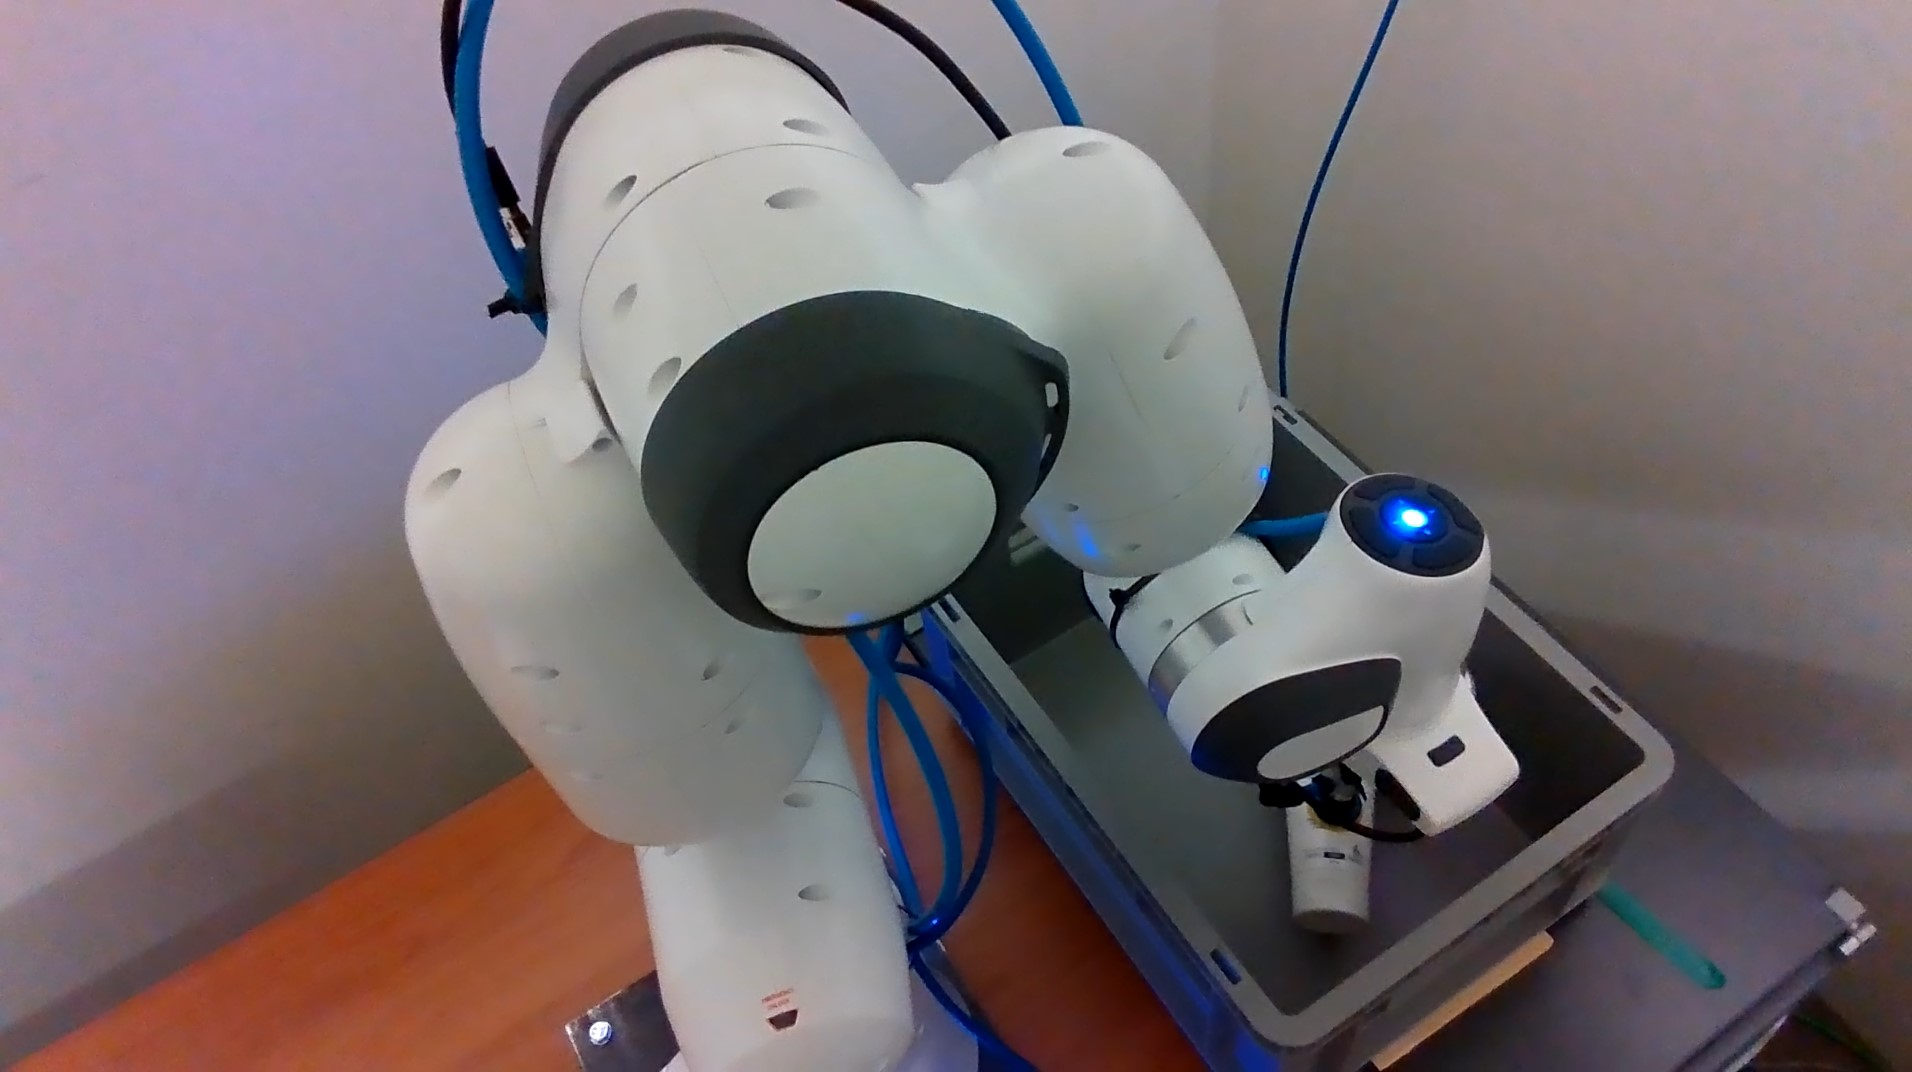
\includegraphics[width=0.3\textwidth]{graphics/results/4above.jpg}}
 \hfill
 \subfloat[Rotates the object and drops it]{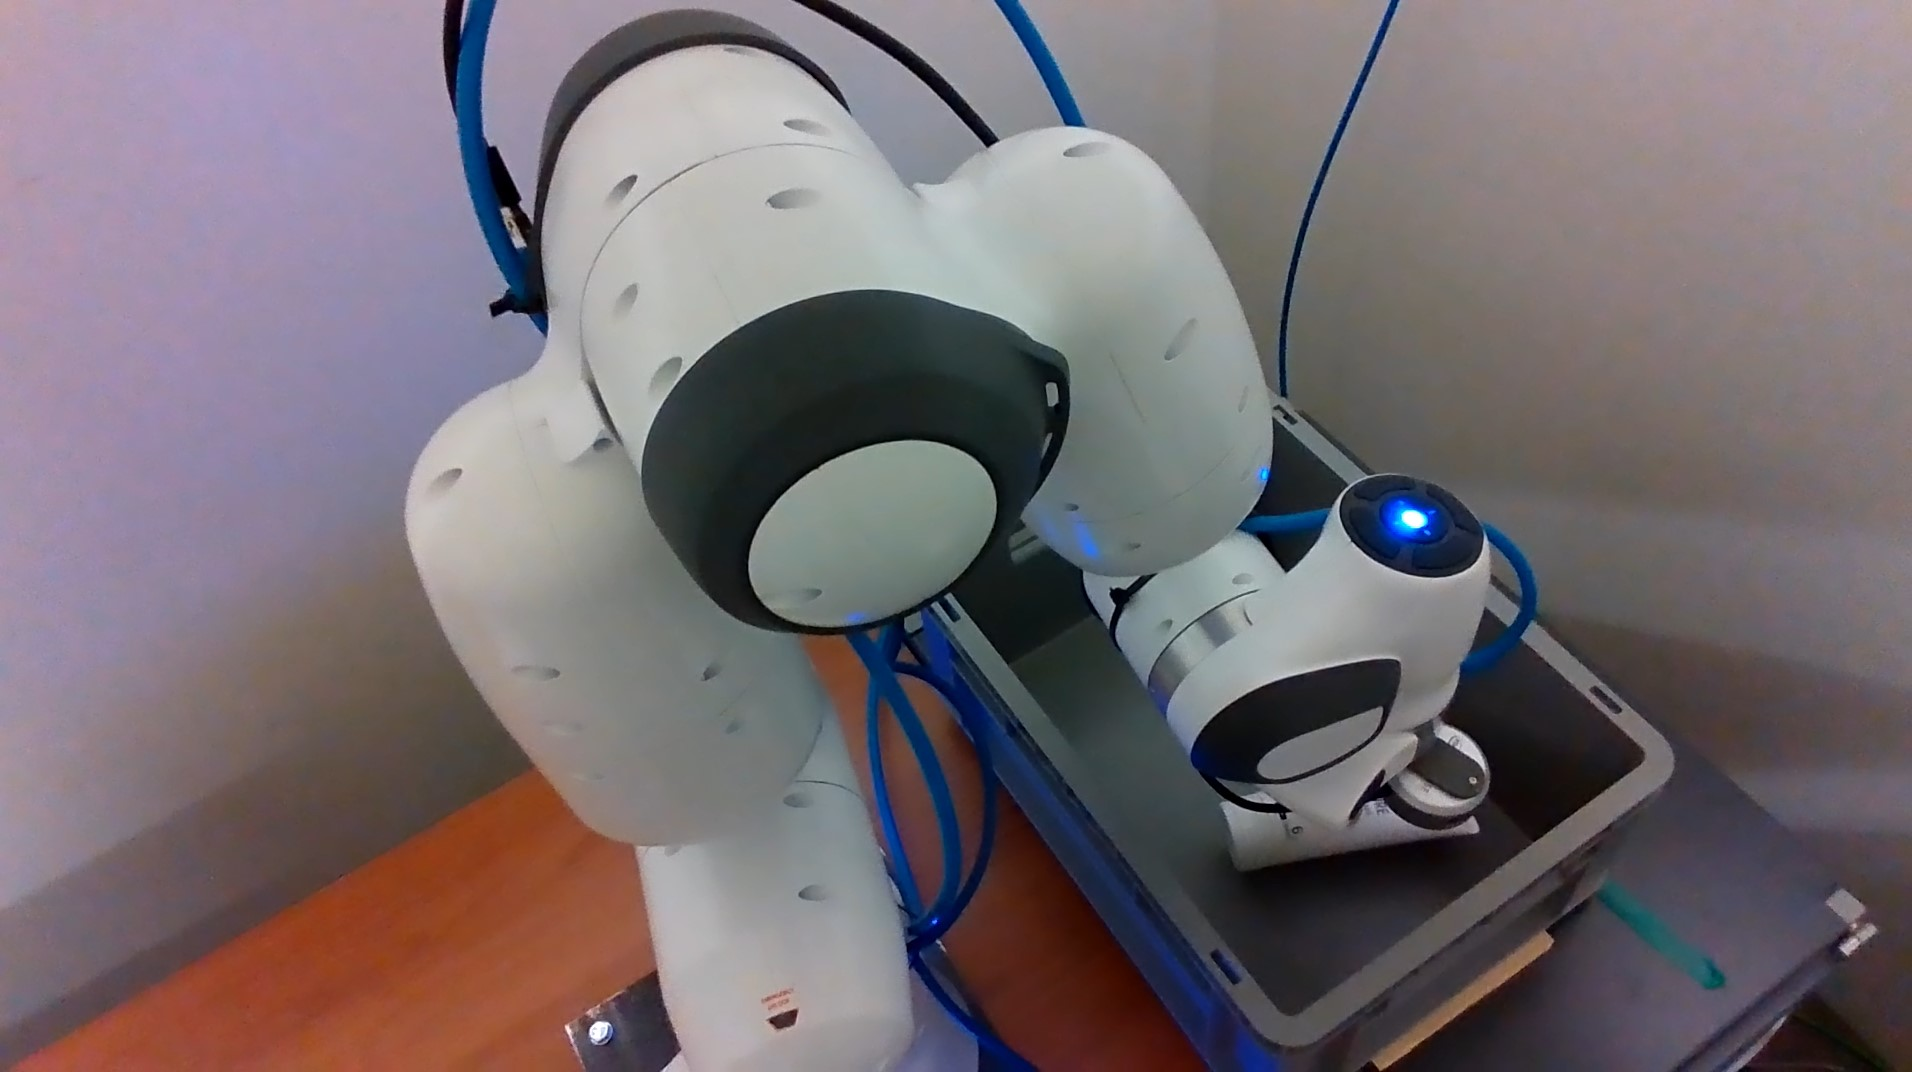
\includegraphics[width=0.3\textwidth]{graphics/results/6rotate.jpg}}
 \hfill
 \subfloat[Goes to home position and capture another image]{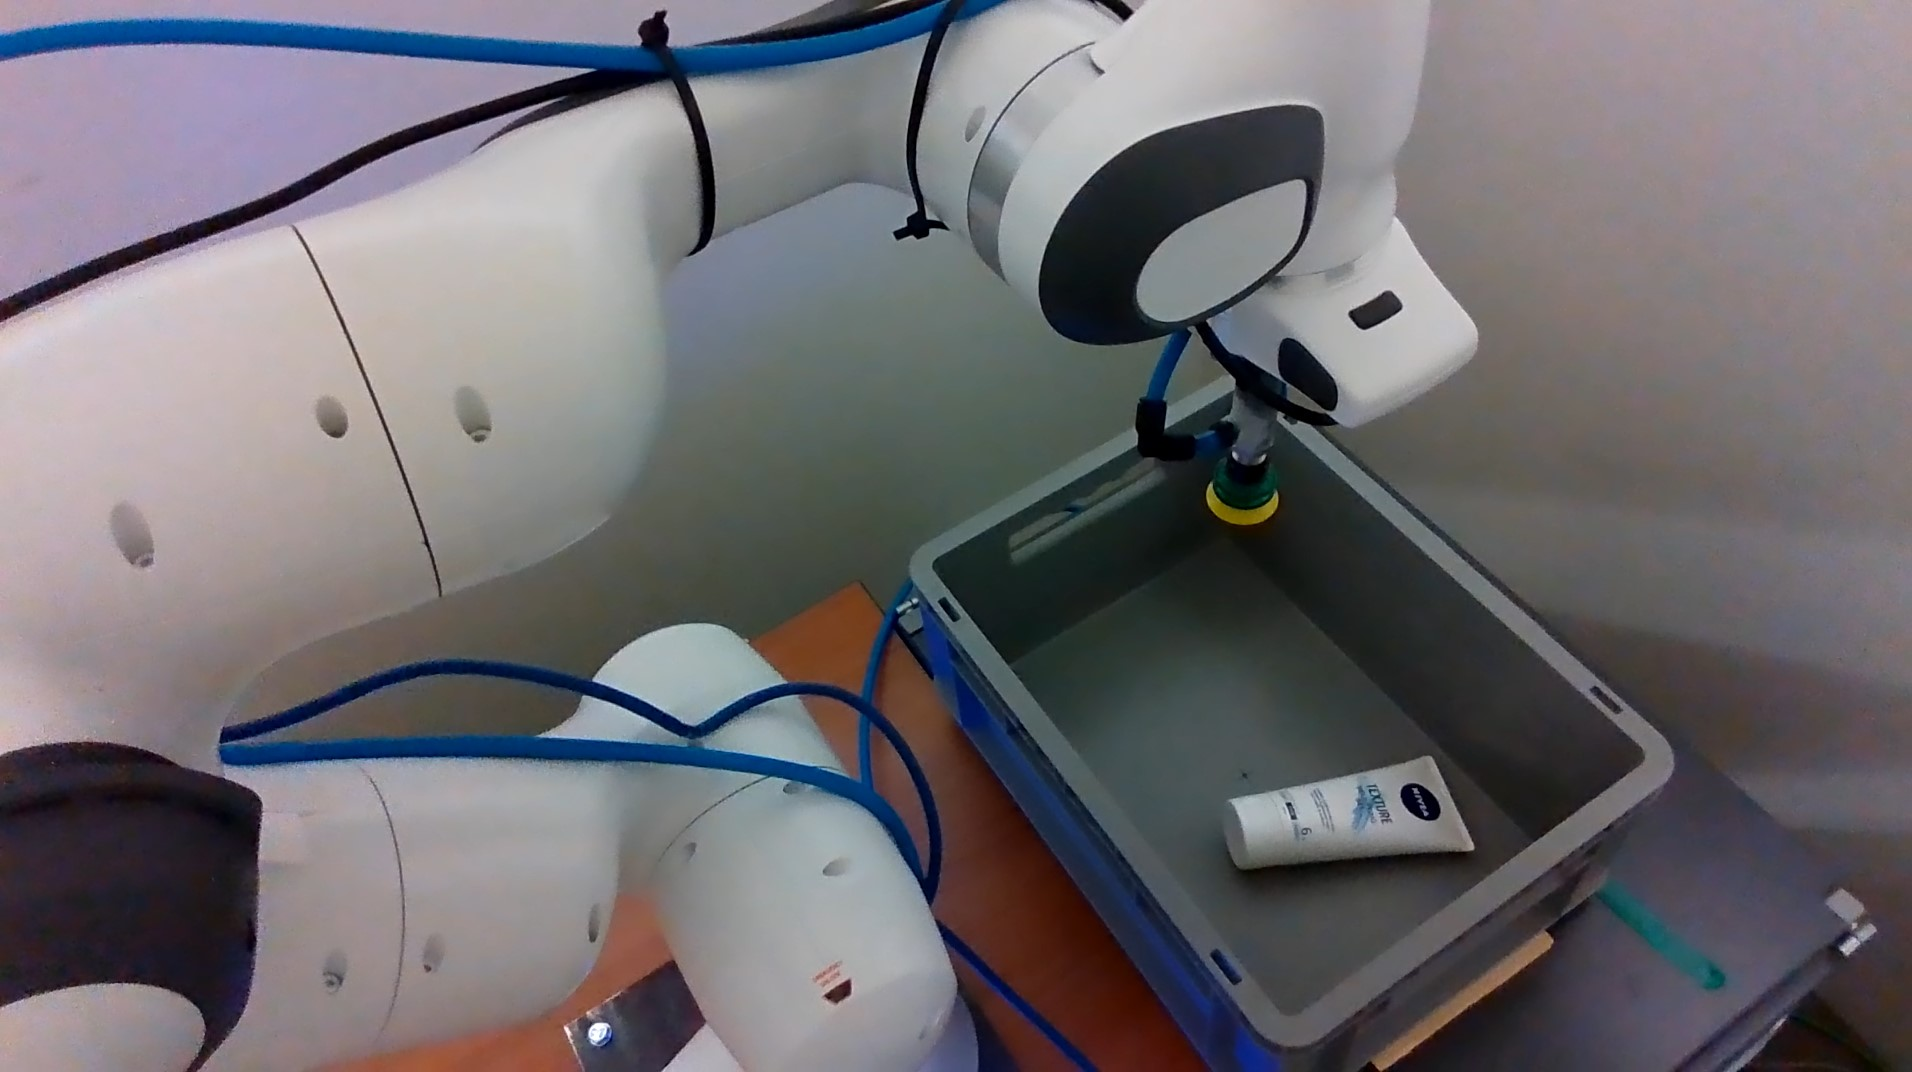
\includegraphics[width=0.3\textwidth]{graphics/results/5drop.jpg}}
 \caption{How the robot software works when there is one object in the bin}
 \label{figure: robotworking}
\end{figure}

\subsubsection{Training images with multiple objects in the bin}
This is the second version of the software, and it picks up one object inside of the bin and moves it to another bin.
The software is controlled by a state machine that has 6 states, which runs while ROS is running. Before going to the state machine the program moves the robot to a fixed home position. 

\vspace{1cm}
\begin{figure}[h]
 \centering
 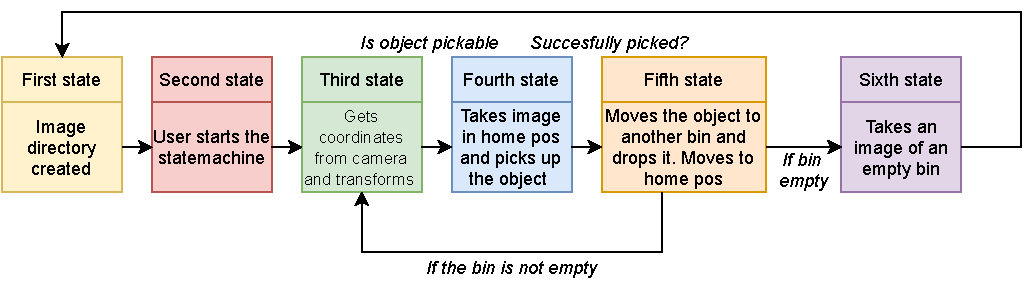
\includegraphics[width=\textwidth]{graphics/statemachine.pdf}
 \caption{State machine diagram}
 \label{fig:statemachine}
\end{figure}

The first state starts by creating a new directory to save the images. 
The second state waits until the user wants coordinates by entering the desired number. 
The third state waits for a message from the find\_pickpoint.py through a ROS topic where it gets an object position from the camera, and then the TF listener transforms the object position in camera coordinates to world coordinates.
The fourth state starts by taking an image of the bin before moving above the object, it then turns on the suction and slowly goes down to the object. The fourth state finishes when the suction pressure increases and that means the suction cup has picked up the object and then moves to a fixed home position.
The fifth state moves the object above another bin, drops it, and ends by going to a fixed home position. When the fifth state has finished and there are items in the bin it goes back to the third state, but if the bin is empty it goes to the sixth state.
The sixth state takes an image of an empty bin and waits until the user wants to start
again with new items in the bin and then goes to the first state again. 


% The software has a loop that runs while ROS is running. 
% Where the robot 
% The TF listener then transforms the object position in camera coordinates to world coordinates. The robots then move to the object position and pick up the object using the suction cup. When the robot has picked up the object successfully it moves the object to another position and rotates the object by a random amount. When the robot has successfully moved the object it goes to the fixed home position and takes an image and saves it into a directory. 
%\fxfatal{Skrifa meira...hvað forritið gerir}
\begin{figure}[h]
 \centering
 % include first image
 \subfloat[Starts in home position, tries to find object using the neural network and capture an image]{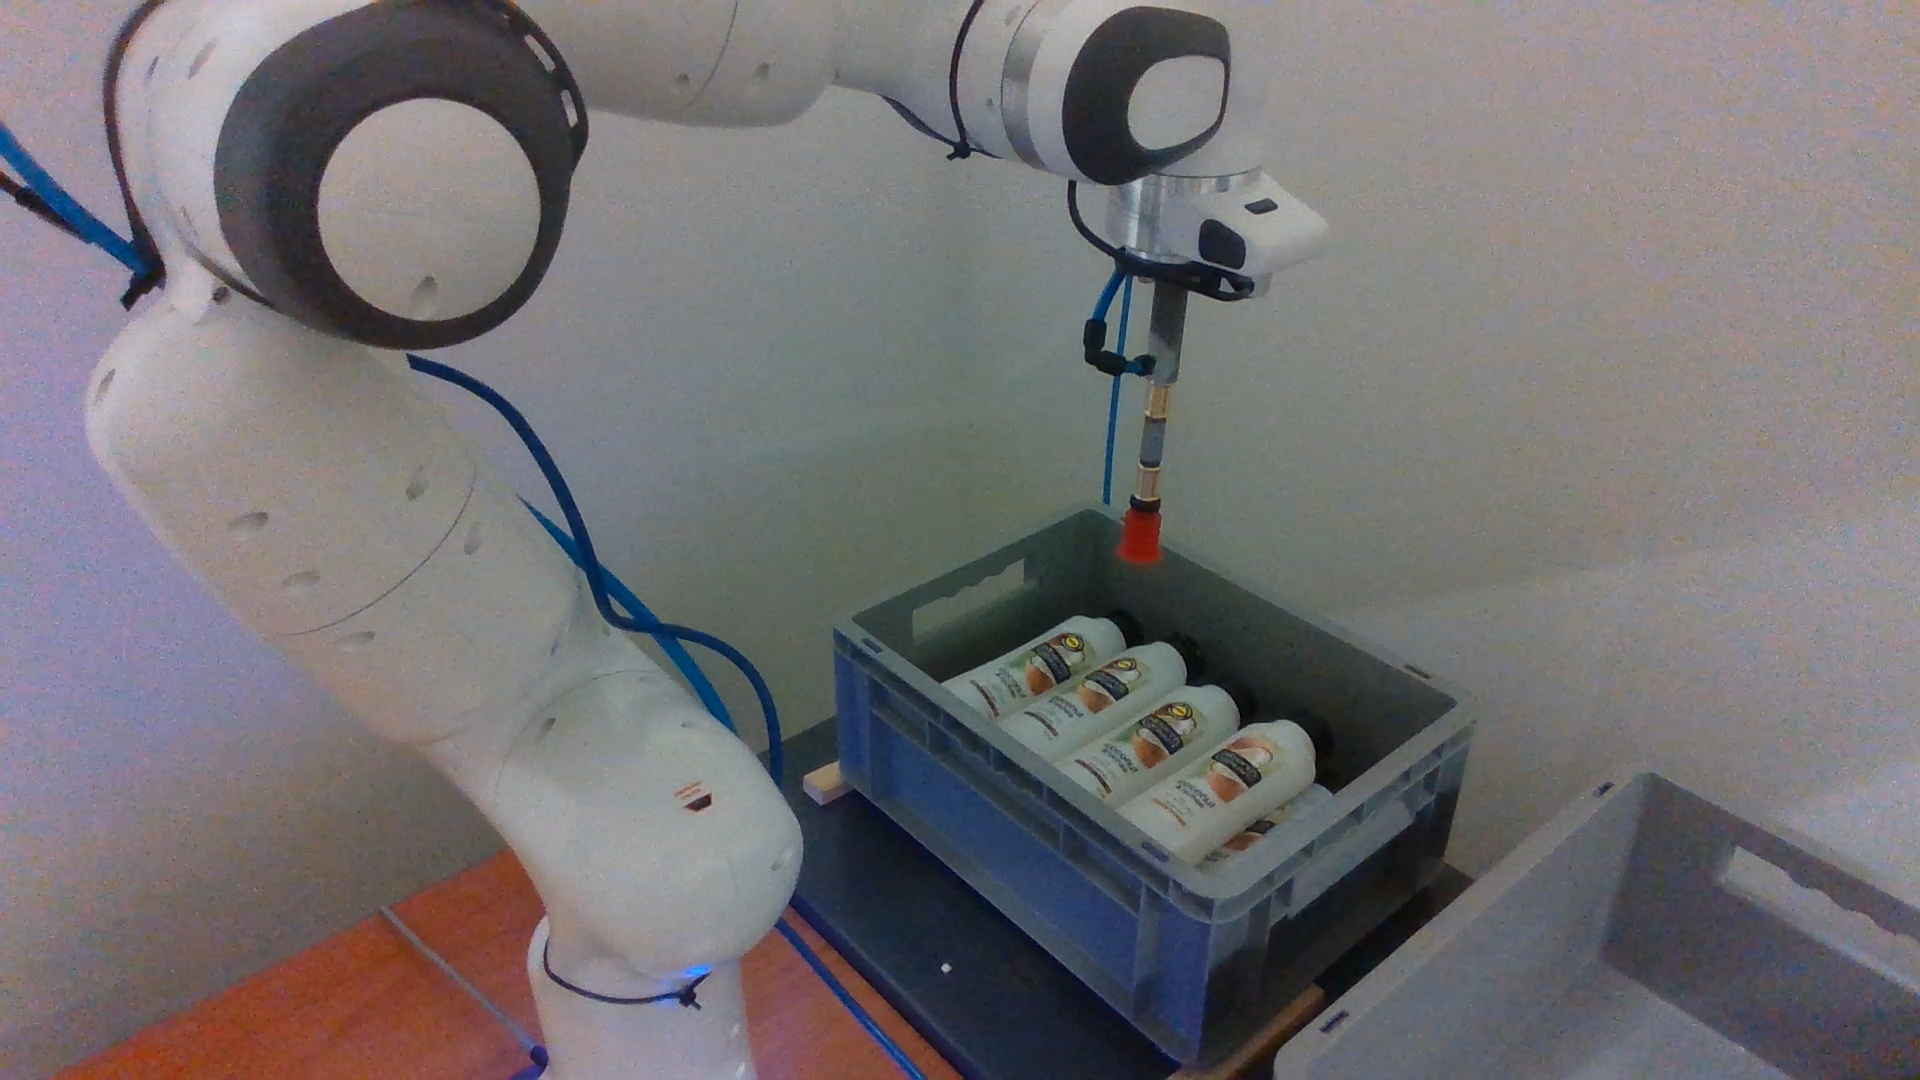
\includegraphics[width=0.3\textwidth]{graphics/results/robotstates/1.png}}
 \hfill
 \subfloat[Goes to the object]{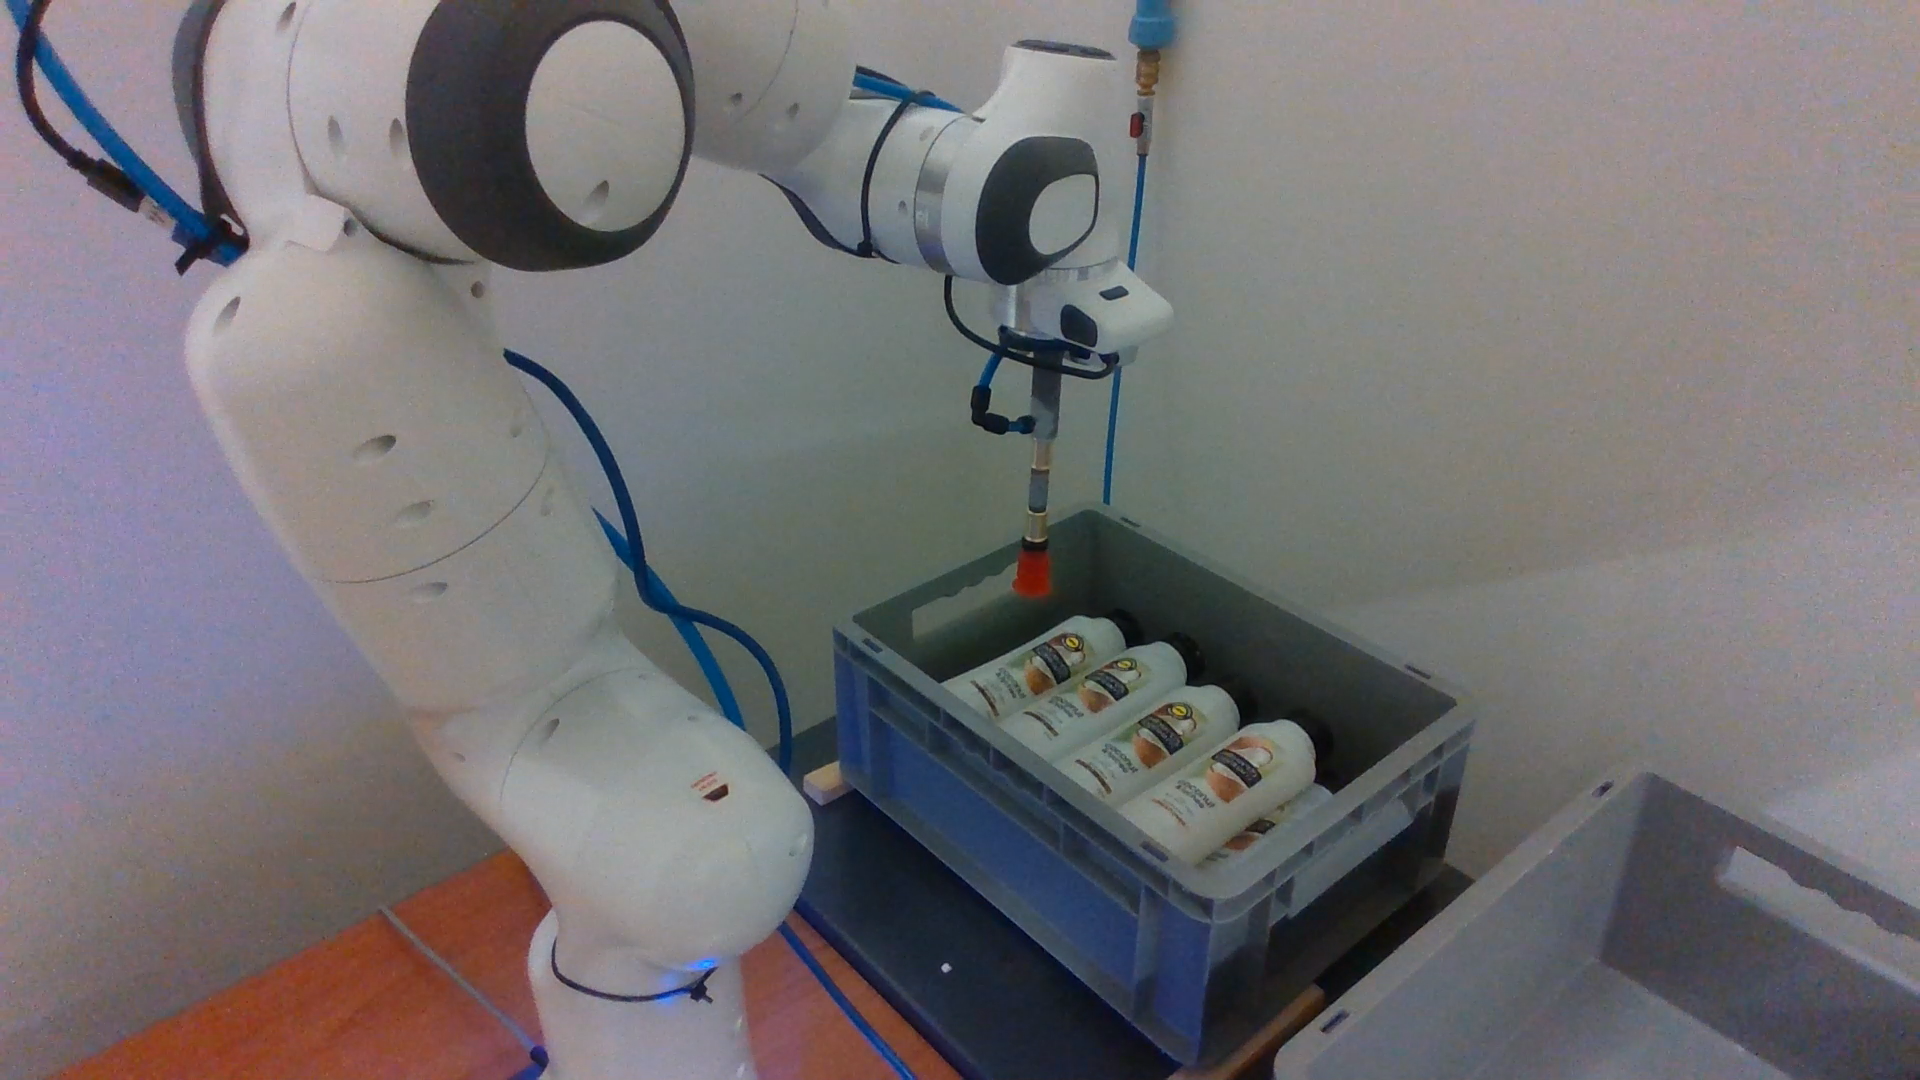
\includegraphics[width=0.3\textwidth]{graphics/results/robotstates/2.png}}
 \hfill
 \subfloat[Picks up the object]{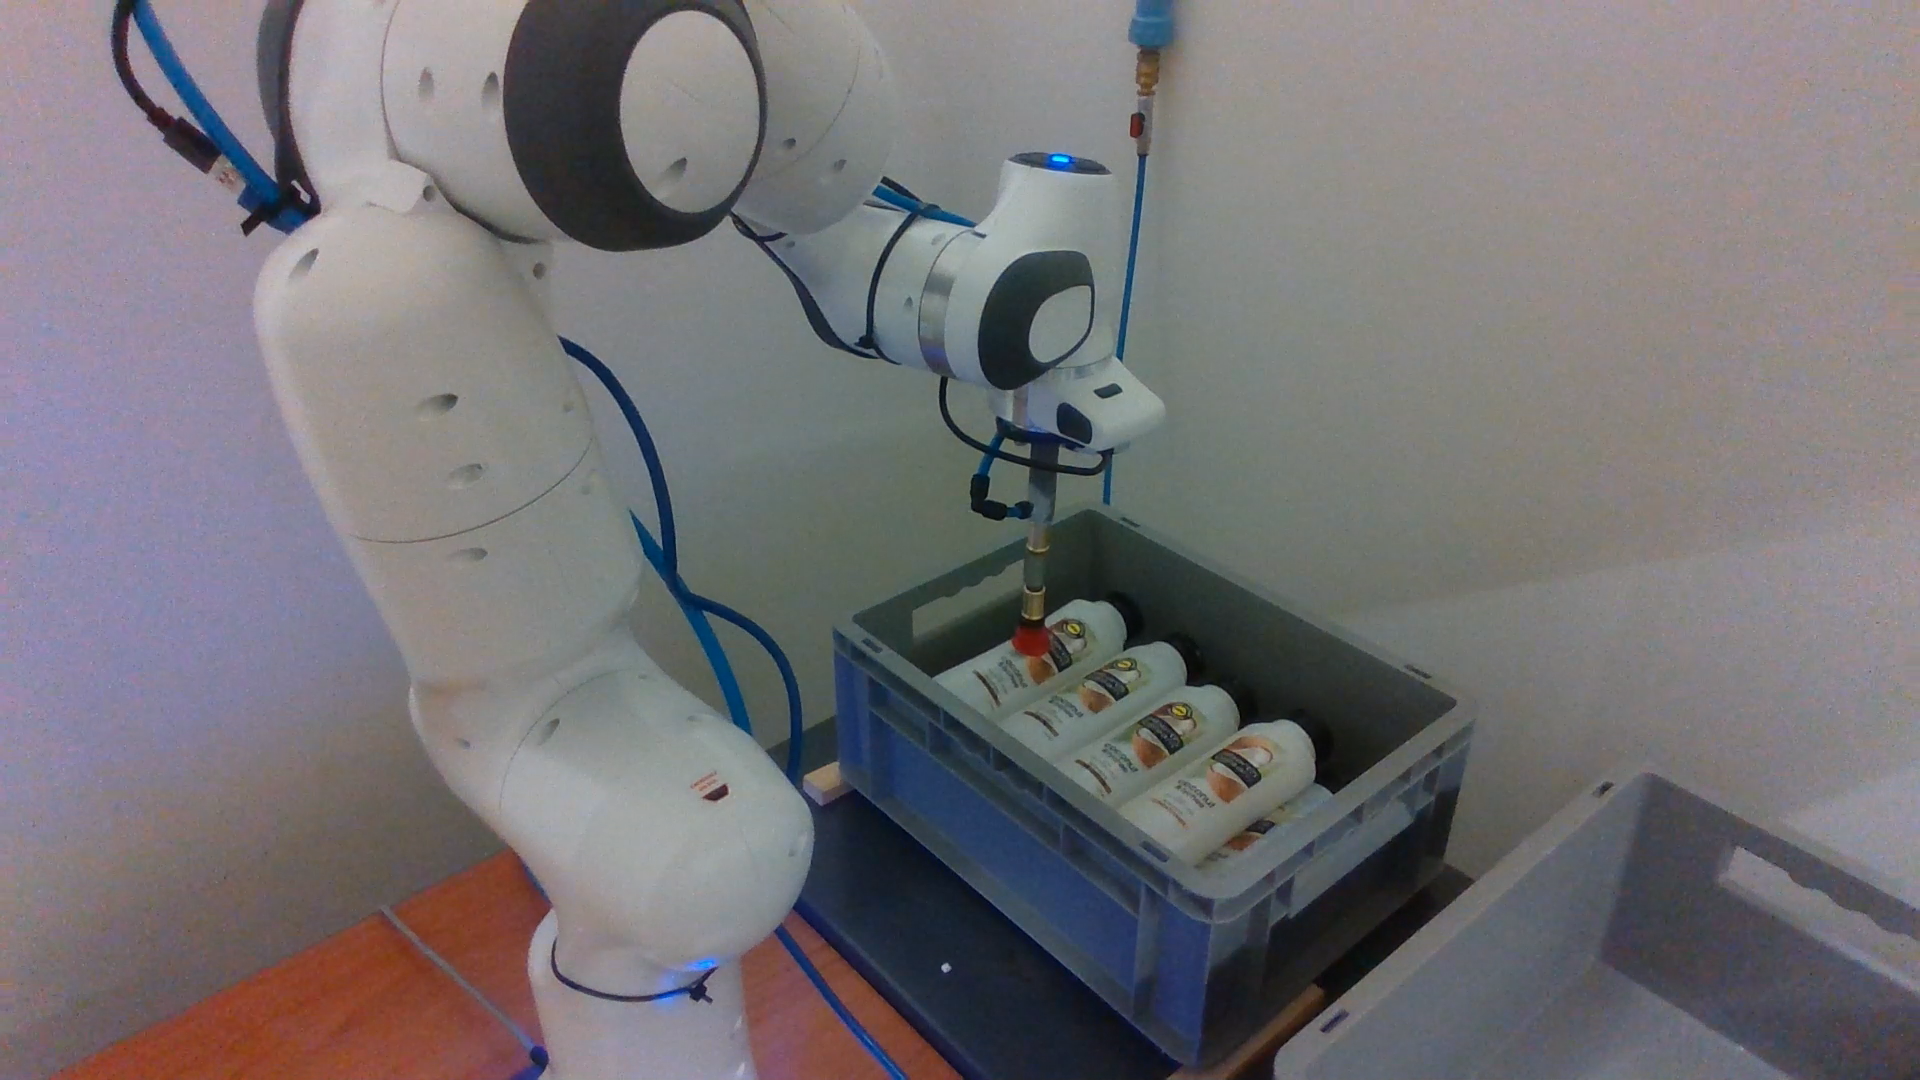
\includegraphics[width=0.3\textwidth]{graphics/results/robotstates/3.png}}
 \hfill
 \subfloat[Moves the object to home position]{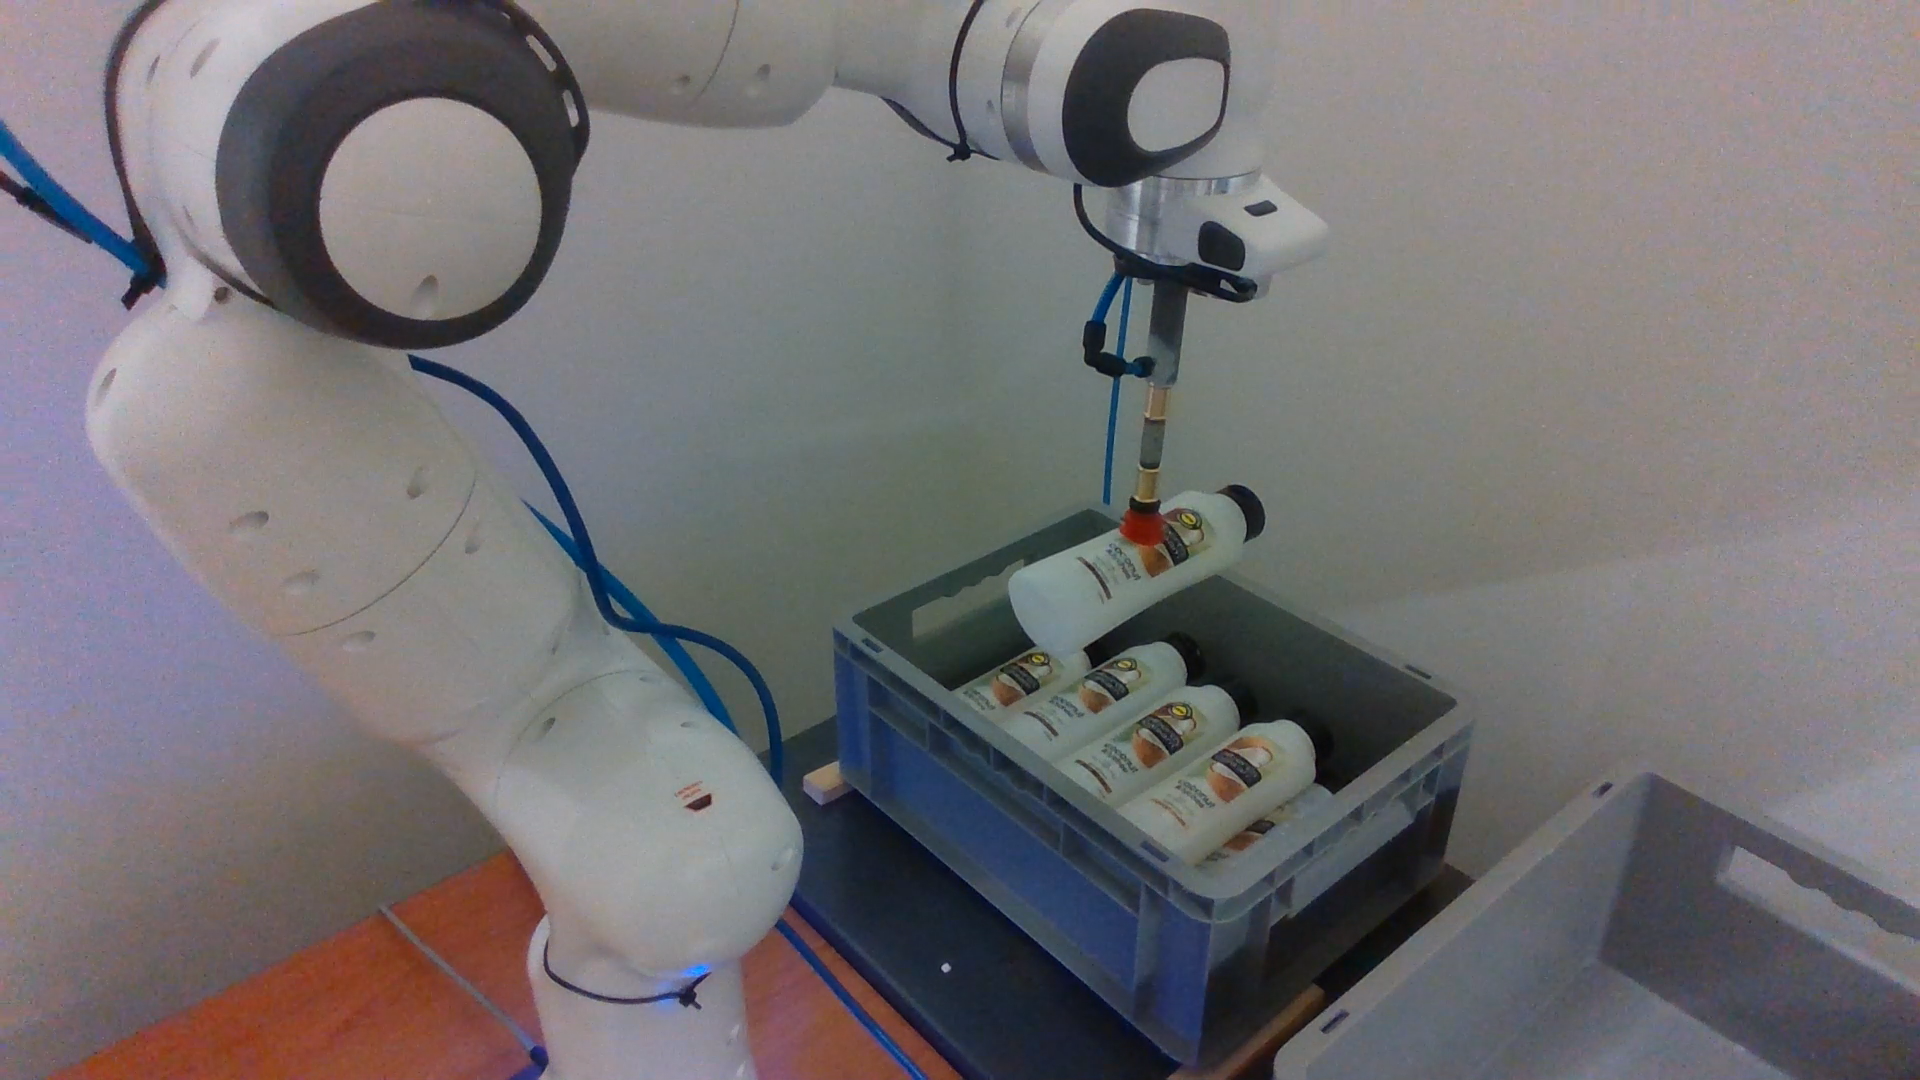
\includegraphics[width=0.3\textwidth]{graphics/results/robotstates/4.png}}
 \hfill
 \subfloat[Moves the object to the other bin and drops it]{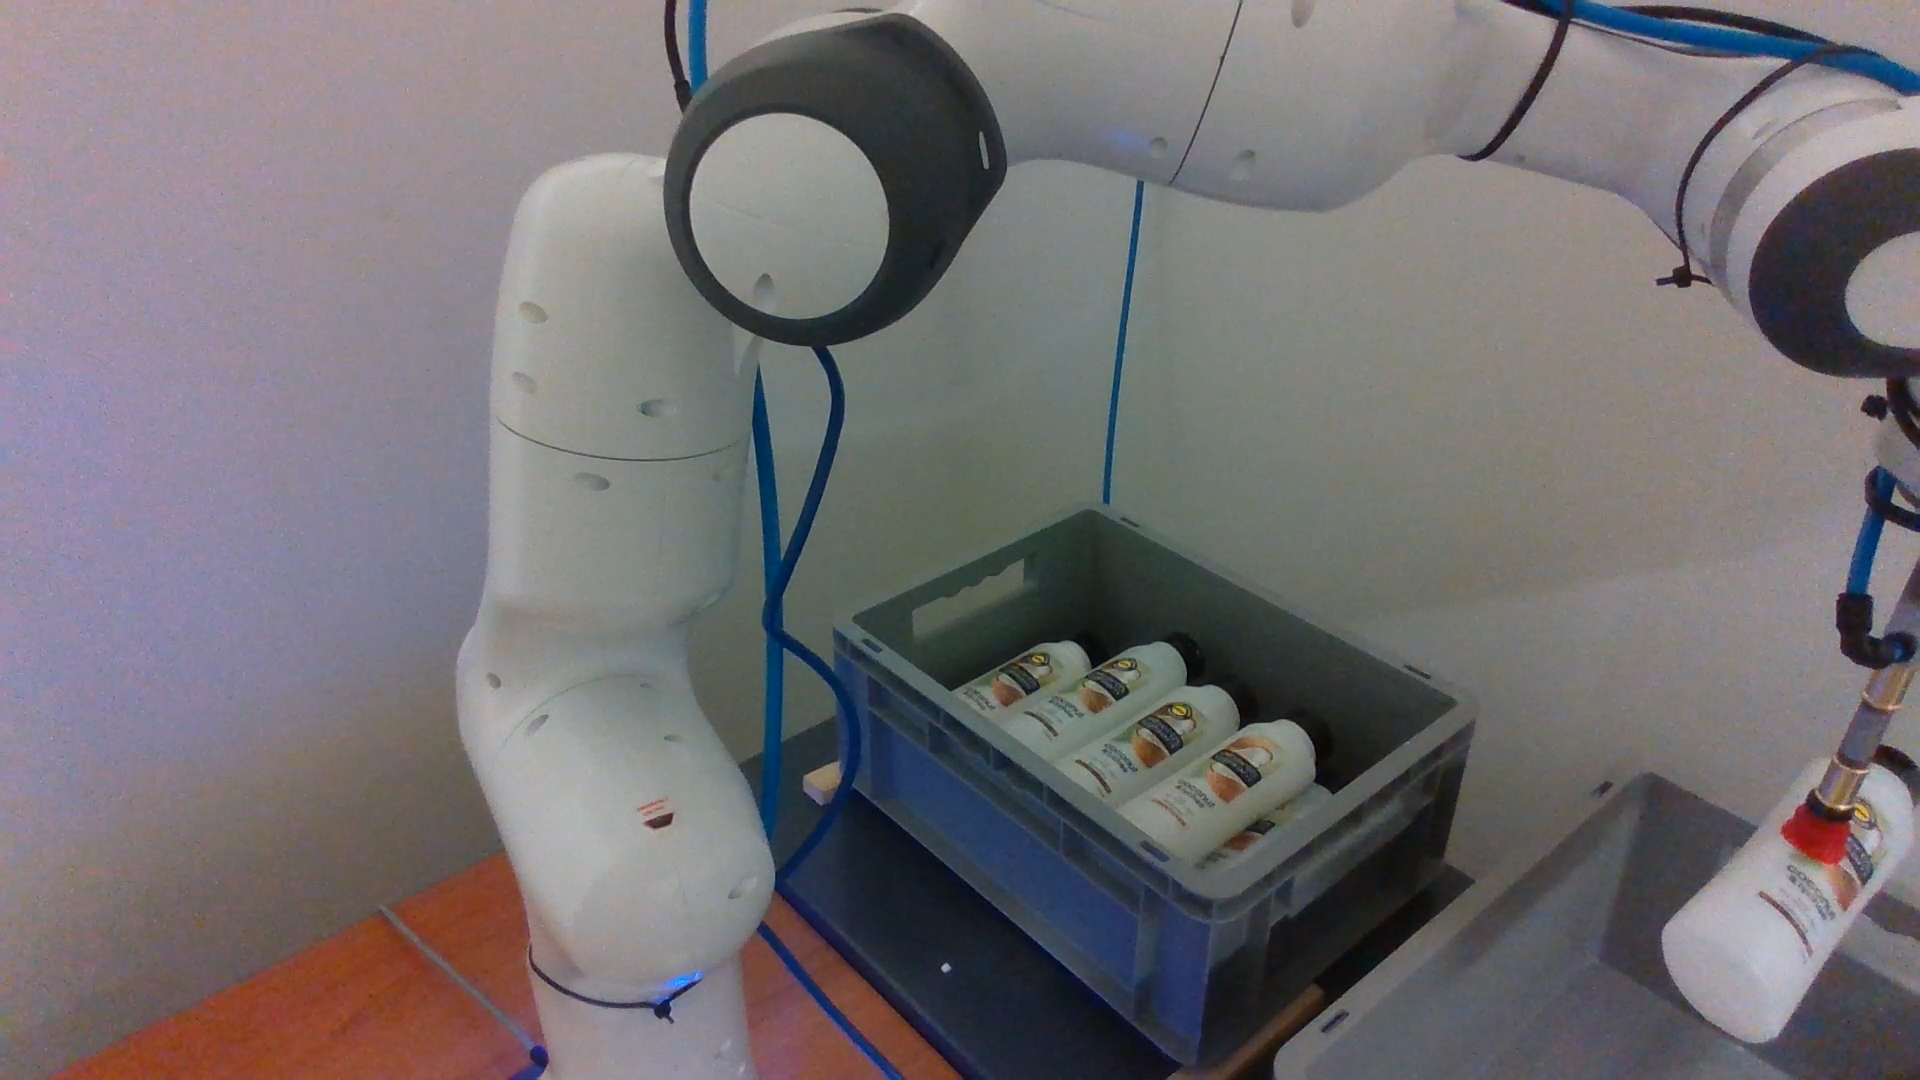
\includegraphics[width=0.3\textwidth]{graphics/results/robotstates/5.png}}
 \hfill
 \subfloat[Goes to home position, capture another image and tries to find new object]{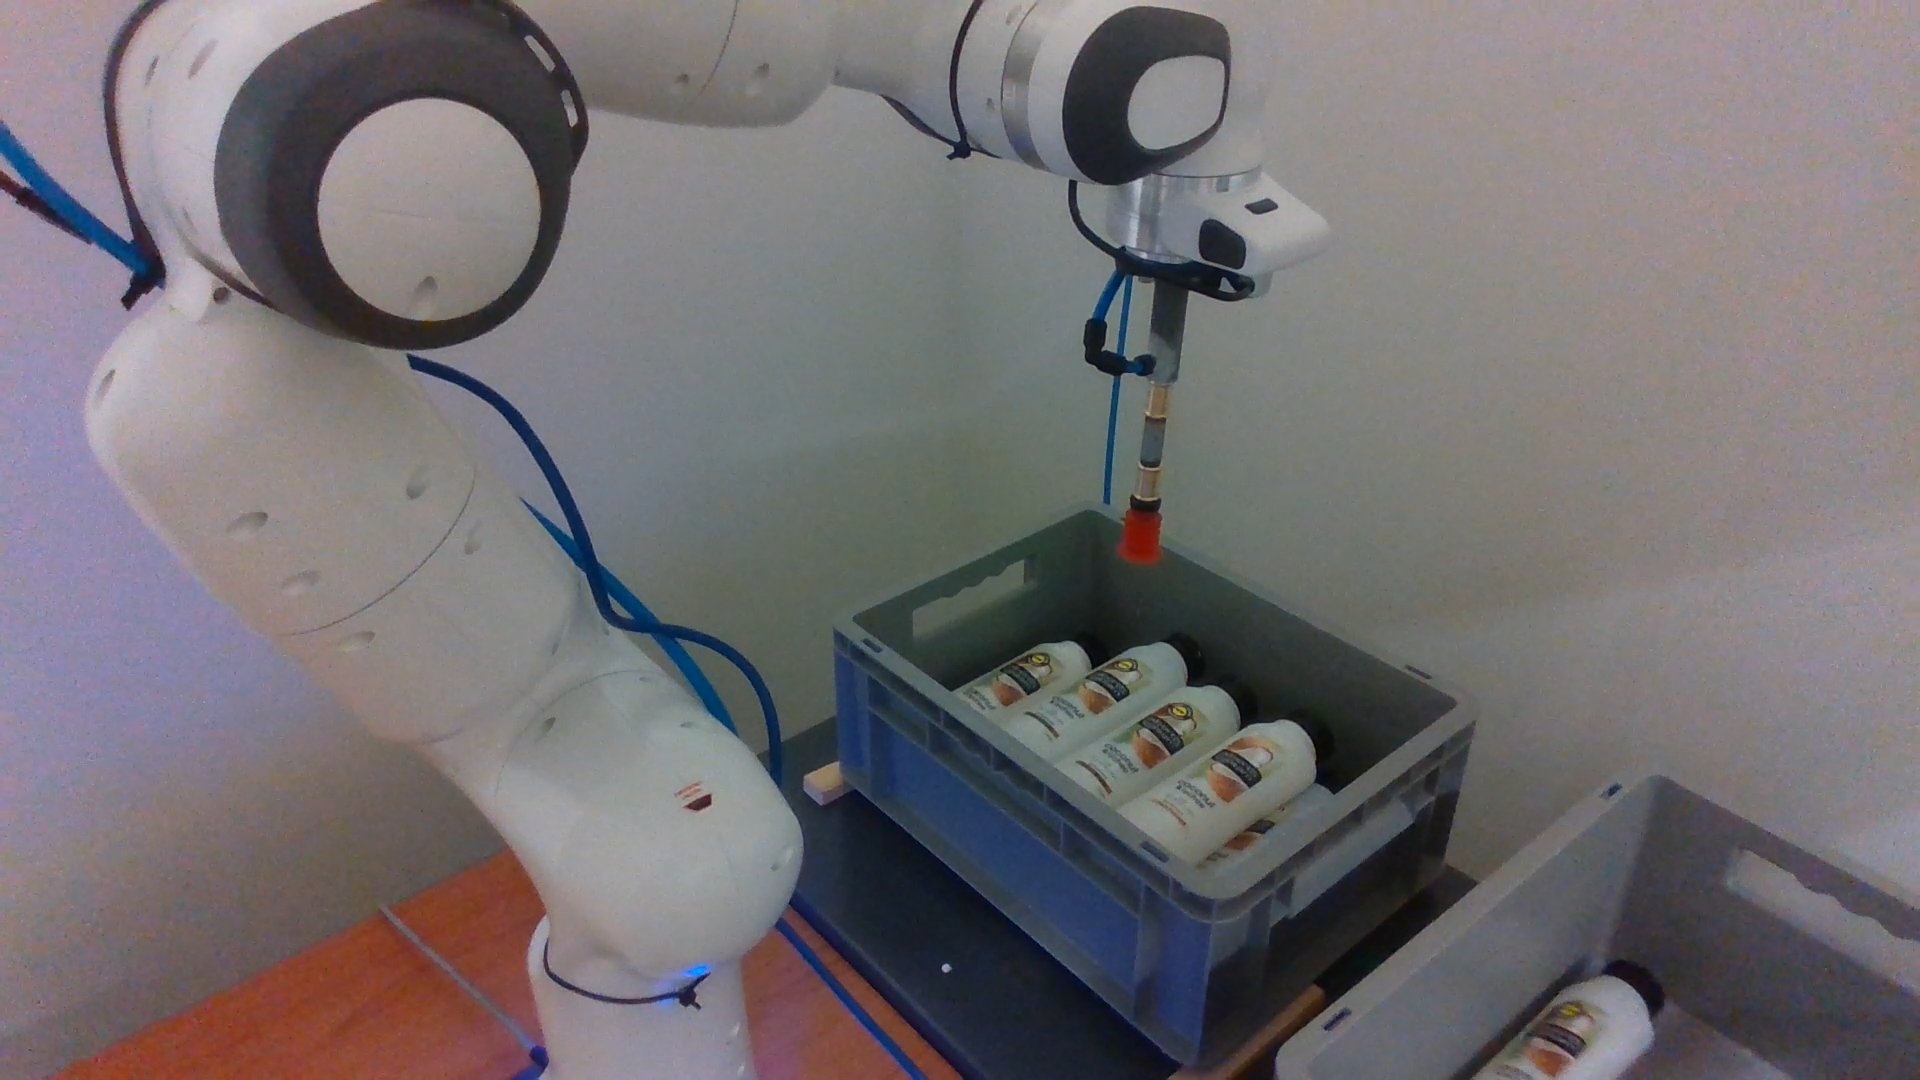
\includegraphics[width=0.3\textwidth]{graphics/results/robotstates/6.png}}
 \caption{How the robot software works when there are multiple object in the bin}
 \label{figure: robotworkingv2}
\end{figure}


\subsection{Image collection and visual guidance}\label{camera}
%\fxfatal{Also make sure that you state clearly that you start from an initial arrangement, in which the object can be detected by the current model, and then proceed to generate (and label) novel arrangements, some of which are not handled by the current model.}
A ROS node was implemented in Python that uses camera images to determine a pick point on an object. The code can be found in the \textit{Appendix \ref{sec:findpickpoint}} known as \textit{find\_pickpoint.py}. 
The program starts by initializing a CVBridge class so it can work on images with OpenCV. It then initializes a neural network, so it can find objects in an image. At last, it creates a subscriber to the "/camera/color/image\_raw" topic with the function "image\_callback" as a callback and creates a publisher "pandaposition" that talks to the robot manipulator. Then a loop keeps the program from shutting down unless ROS is shut down.

When the callback gets an image it waits for an aligned depth to a color image so it can read a depth at a certain point. It then goes into a find objects function that finds the object in the image using the neural network, which locates the center of an object. When the program has found pixel coordinates of the object it can find the depth at that point and can create real-world coordinates(X, Y, Z) in meters at the camera location. At last, the programs send the real-world coordinates to a "pandaposition" publisher so the robot manipulator uses the coordinates.

\begin{figure}[h]
 \centering
 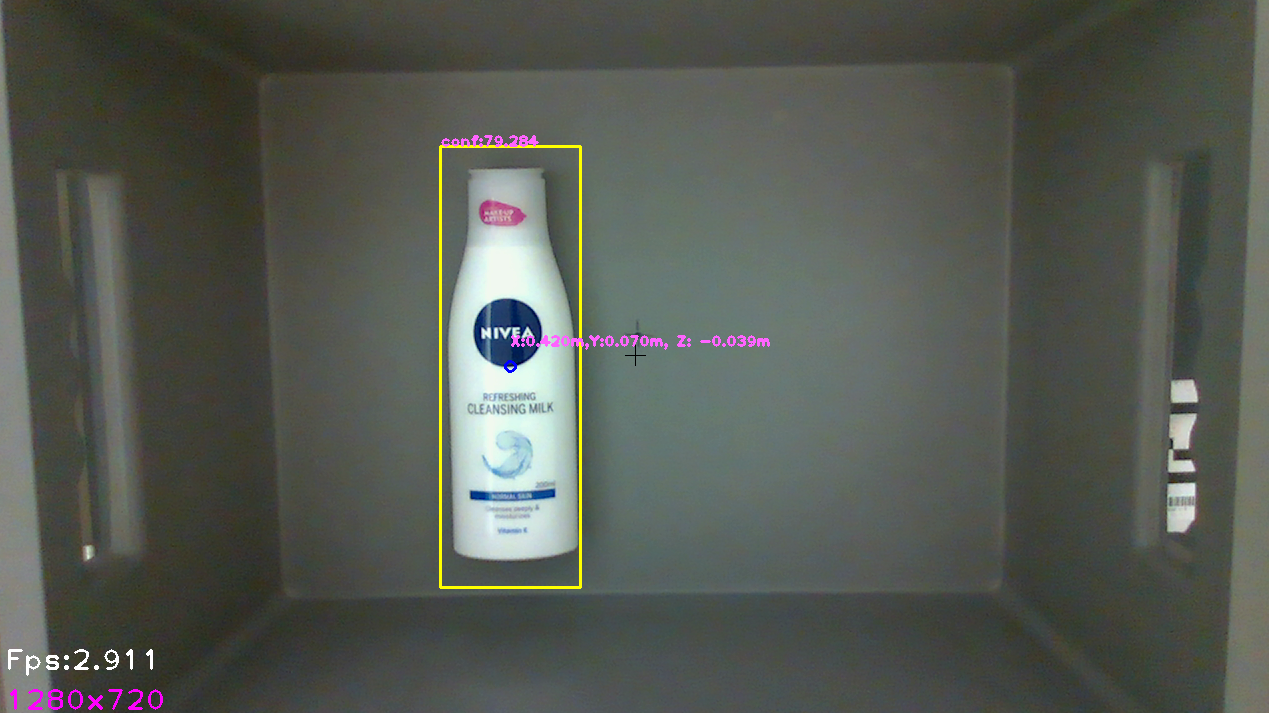
\includegraphics[width=0.8\textwidth]{graphics/findpickpoint.png}
 \caption{An example of the output from the find\_pickpoint.py code}
 \label{fig:findpickpoint}
\end{figure}

From \textit{Figure \ref{fig:findpickpoint}} you can see the confidence, frames per second(Fps), image size, X which is forward length or depth, Y and Z is the distance from the center of the camera in meters. 
The camera coordinates system can been seen in \textit{Figure \ref{fig:l515cor}}.


\subsection{Automatic image labelling}\label{labelimg}

The difference of two images taken before and after an object is moved was used to determine the extent of the objects in the two images. This allowed an annotation in the form of an object mask or a bounding box to be generated automatically. The software can be found in the \textit{Appendix \ref{sec:difference}}, as \textit{difference.py}.

% When the robot manipulator and camera had captured images from a fixed home position, the images were put in software called \textit{difference.py} which finds the difference between images and can be found in the \textit{Appendix \ref{sec:difference}}. That program was coded in Python and works individually. The program locates objects in the images and labels them. 
\subsubsection*{Before vs. After}\label{beforeandafter}
The first method used before- and after- image, the bottle was moved to the other side and then found the difference. It calculates the Structural Similarity Index (SSIM) between the two images, SSIM\cite{datta_all_2020} is used as a metric to measure the similarity between two given images. The OpenCV threshold and contours were used to draw the contours. Then iterate around the contour area, and get a bounding area and draw a rectangle around.
An example of input images can been seen in \textit{Figure \ref{figure: beforeafter}}, and try's to find the difference between before and after.
\begin{figure}[h]
 \centering
 % include first image
 \subfloat[Before]{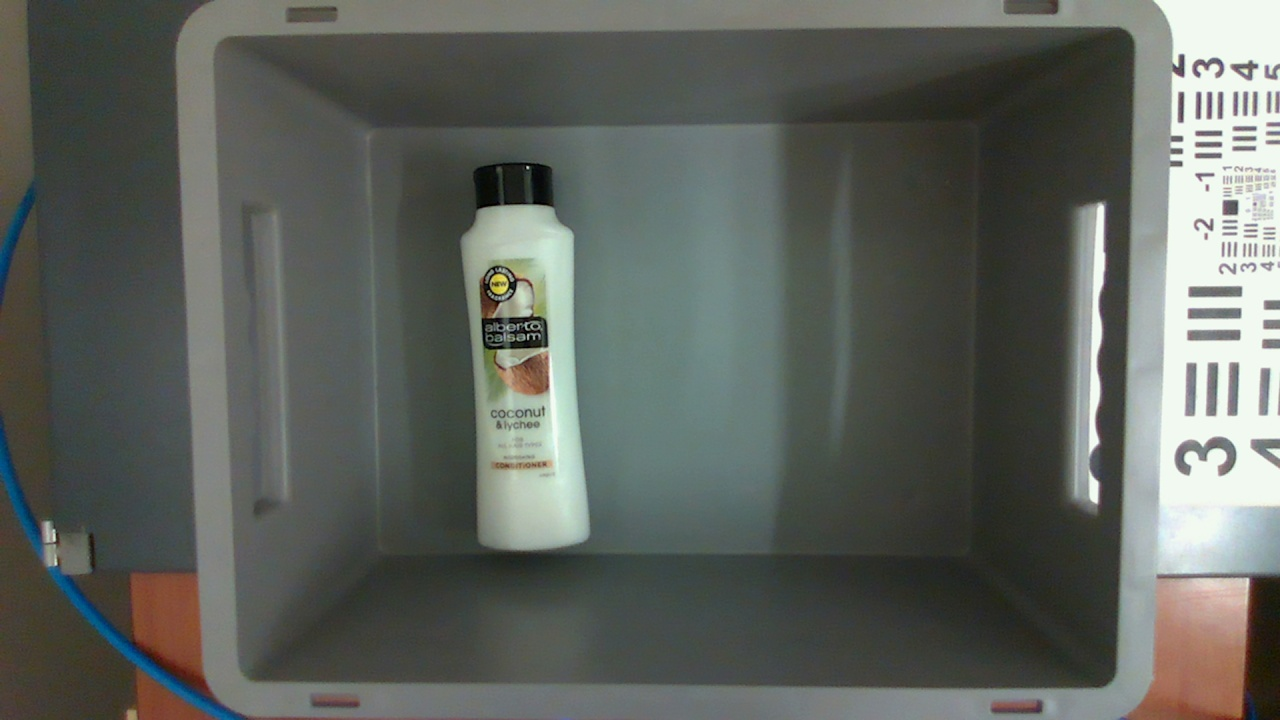
\includegraphics[width=0.495\textwidth]{graphics/methods/frame0000.jpg}}
 \hfill
 \subfloat[After]{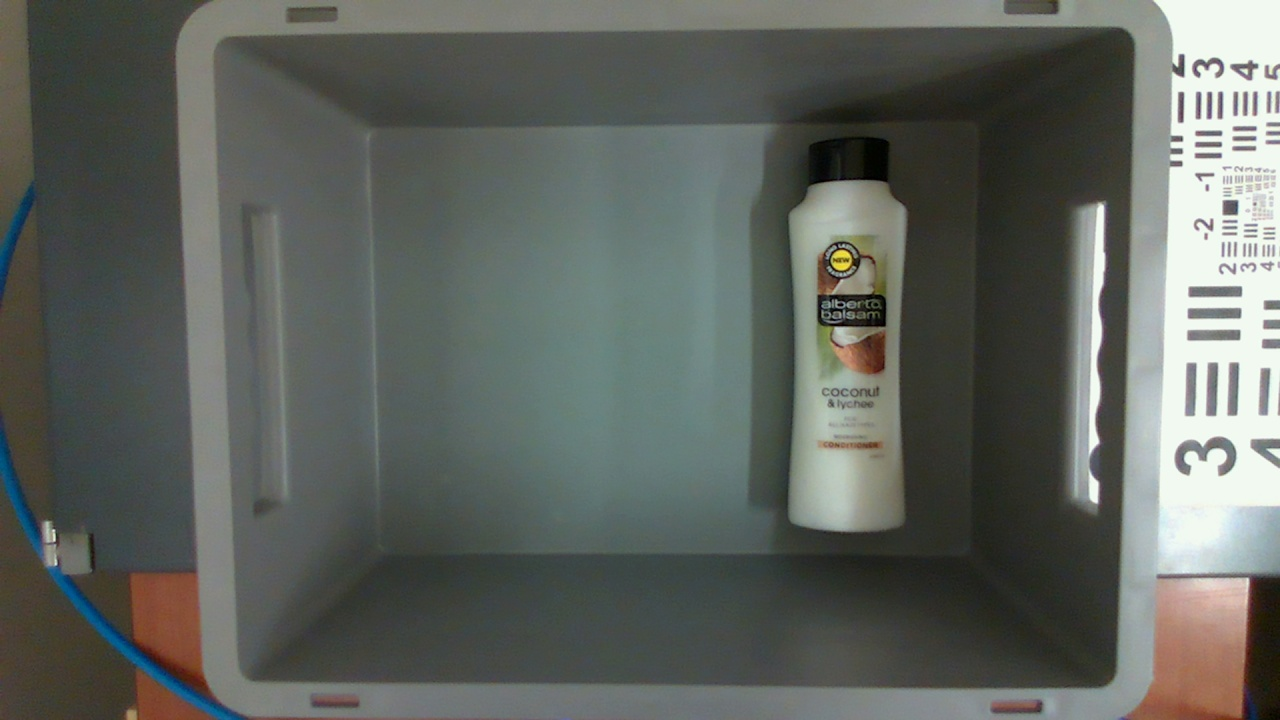
\includegraphics[width=0.495\textwidth]{graphics/methods/frame0001.jpg}}
 \caption{An example of input images}
 \label{figure: beforeafter}
\end{figure}

\subsubsection*{Empty bin vs. item in the bin}\label{emptyvsitem}
The second method uses two functions to find objects in the image, one is to find the difference between an empty bin and a bin with an object inside and the other is to find contours in the image. 
The function that delivers results that are under the bounding box boundaries, then that function is used. If the results are similar, average values are used.
When the objects have strange colors, such as a bottle with both white and black the contours are not that good, and that is why there are two functions so there will be no bad results. 
In this program, OpenCV and Skicit-image are used. An example of input images can been seen in \textit{Figure \ref{figure: emptyafter}}.
\begin{figure}[h]
 \centering
 % include first image
 \subfloat[Empty bin]{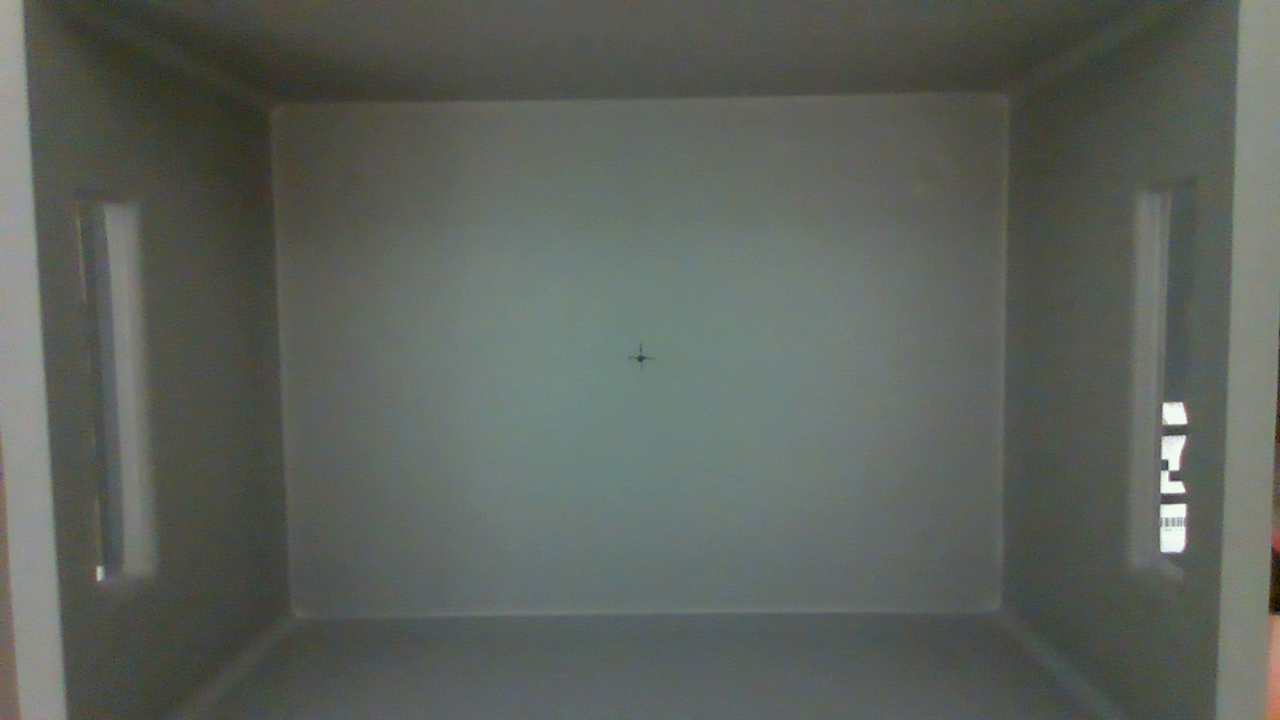
\includegraphics[width=0.495\textwidth]{graphics/methods/0000.png}}
 \hfill
 \subfloat[Item in the bin]{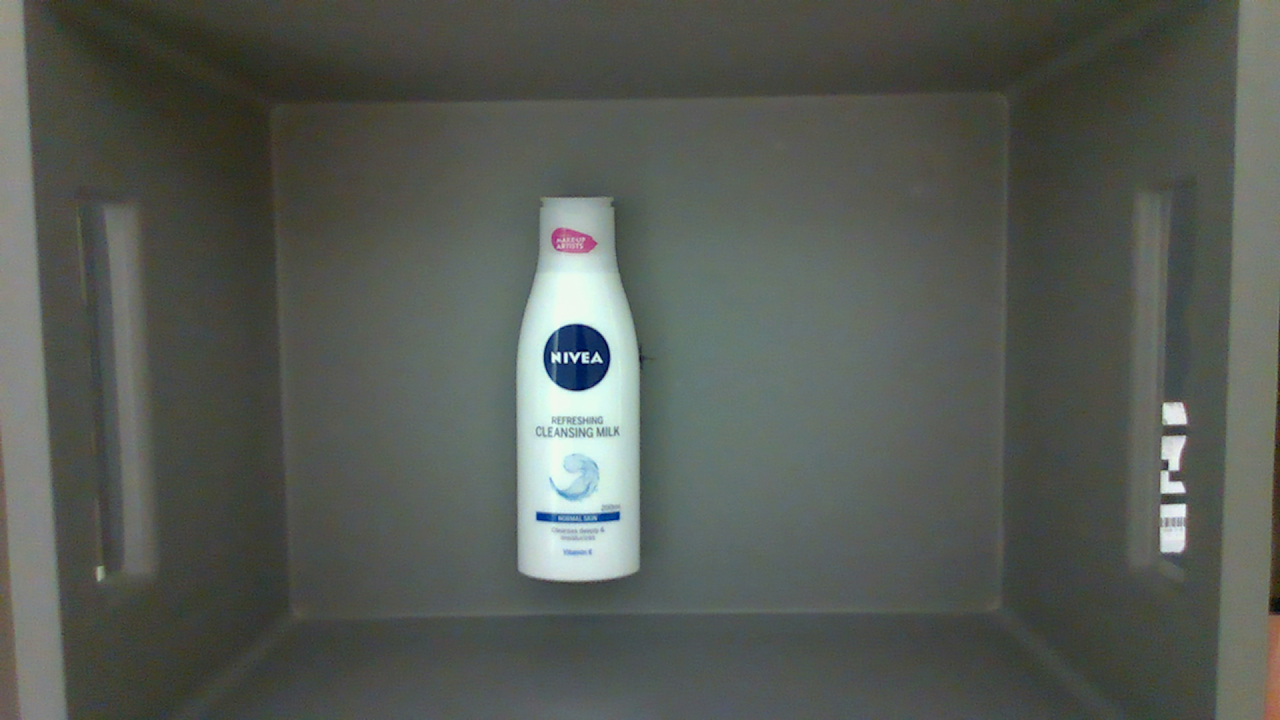
\includegraphics[width=0.495\textwidth]{graphics/methods/0001.png}}
 \caption{An example of input images}
 \label{figure: emptyafter}
\end{figure}

So the program starts by getting an image of an empty bin and then the images with an object in it. 
Then it finds uses \textit{cv2.Canny} to find the edges, creates a binary threshold image with \textit{cv2.threshold} and finds the contours from the threshold image. 
When the contours have been found it goes to a function that checks if the contour has four corners to check if it is a rectangle. 
If it has four corners and the area is within area marks it saves the location\textit{(center point, width, and height relative to the image size)} of the object in a text file named the same as the image. 
When the program has finished with the all images an text file with locations of objects for each image, is saved and can be used to train the neural network. 


%%%%%%%%%%%%%%%%%%%%%%%%%%%%%%%%%%%%%%%%%%%%%
\clearpage
\section{Datasets}
Annotated datasets are intended to add metadata to a dataset. The metadata is normally tagged. Tags may be added to any data type, including texts, images, and videos. There are many ready-made datasets online such as the COCO - Common objects in context \cite{noauthor_what_nodate} and Google’s Open Images dataset \cite{noauthor_open_nodate}.

Most ready-made datasets for object detection are better suited for self-driving cars and image classification. They focus more on items such as people, animals, and large objects such as cars and bikes. For this project, the emphasis was on objects that are sold at online retails stores.

\subsection{Automatically generated dataset with one object in the bin} \label{sec:firstdataset}
The first dataset was created using bottles that have been used in experiments at the Robot Interaction Lab. It included 4 types of products and consists of 376 images, \textit{Alberto Balsam}(101 images), \textit{Nivea Cleansing Milk}(102 images), \textit{Nivea Elastic}(72 images) and \textit{Nivea Texture}(101 images). 
This is a robot-generated dataset with automatically generated labels, which has only one object in the bin. 
These products were moved, rotated, and then captured in the home position to achieve more images to add to the dataset. 
These products can be seen in \textit{Figure \ref{figure: products}}.

\begin{figure}[h]
 \centering
 % include first image
 \subfloat[Alberto Balsam ]{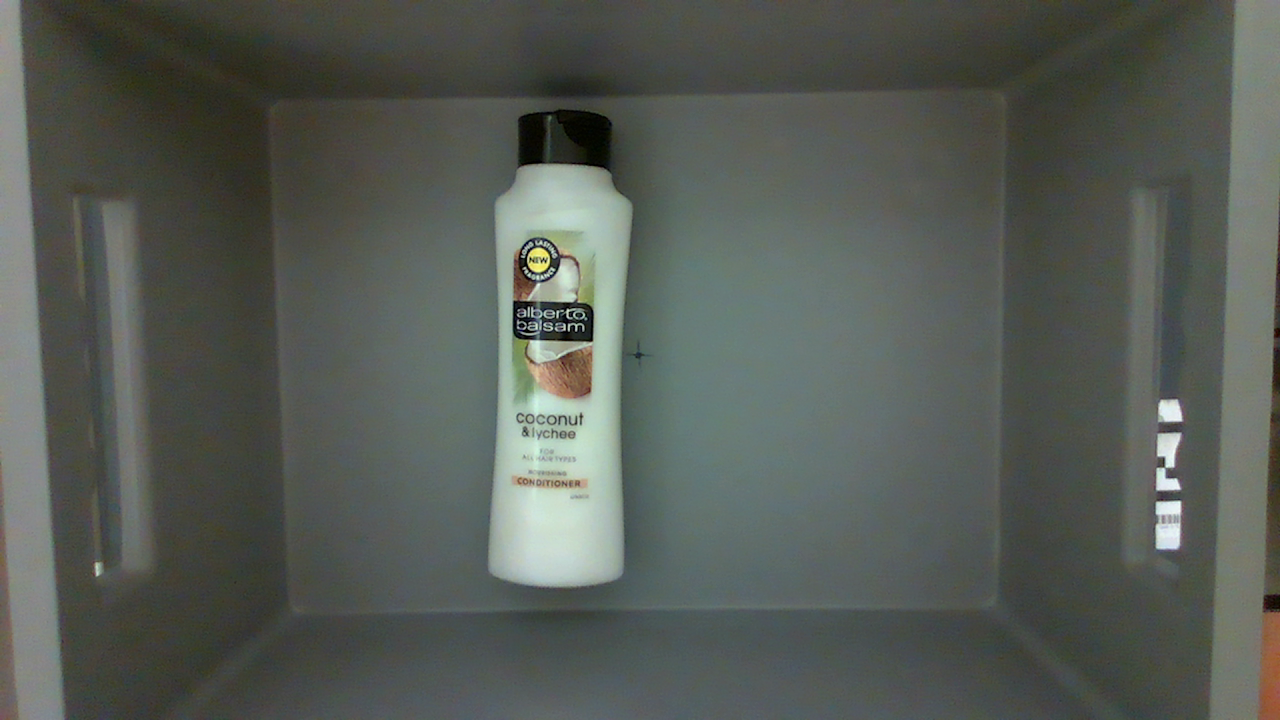
\includegraphics[width=0.5\textwidth]{graphics/methods/b0001.png}}
 \hfill
 %\hspace{2 cm}
 \subfloat[Nivea Cleansing Milk]{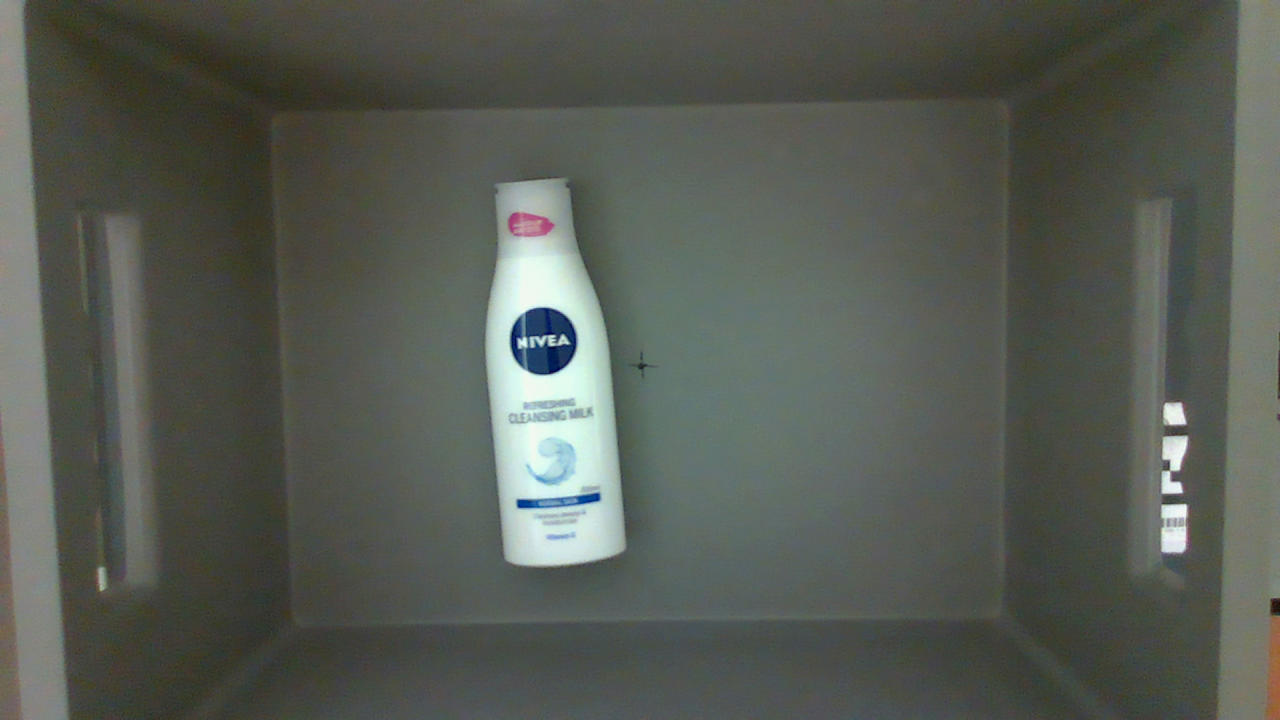
\includegraphics[width=0.5\textwidth]{graphics/methods/b0144.png}}
 \hfill
 %\hspace{2 cm}
 \subfloat[Nivea Elastic]{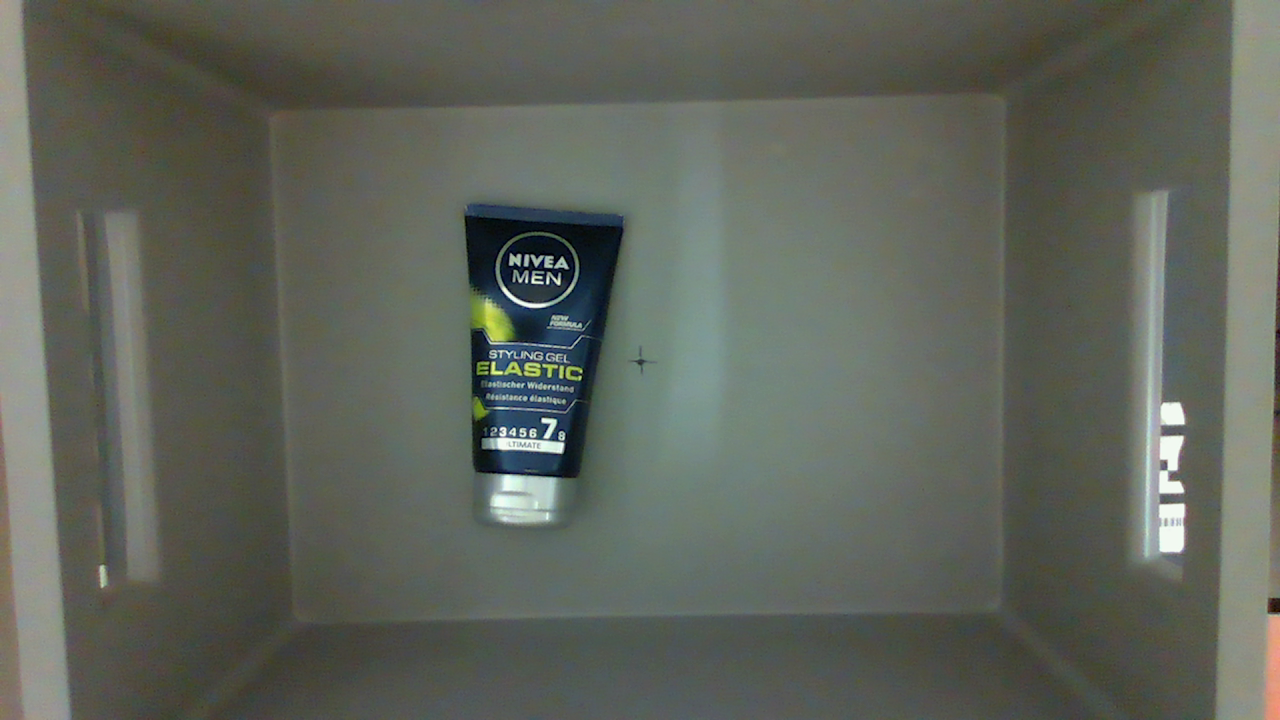
\includegraphics[width=0.5\textwidth]{graphics/methods/b0209.png}}
 \hfill
 %\hspace{2 cm}
 \subfloat[Nivea Texture]{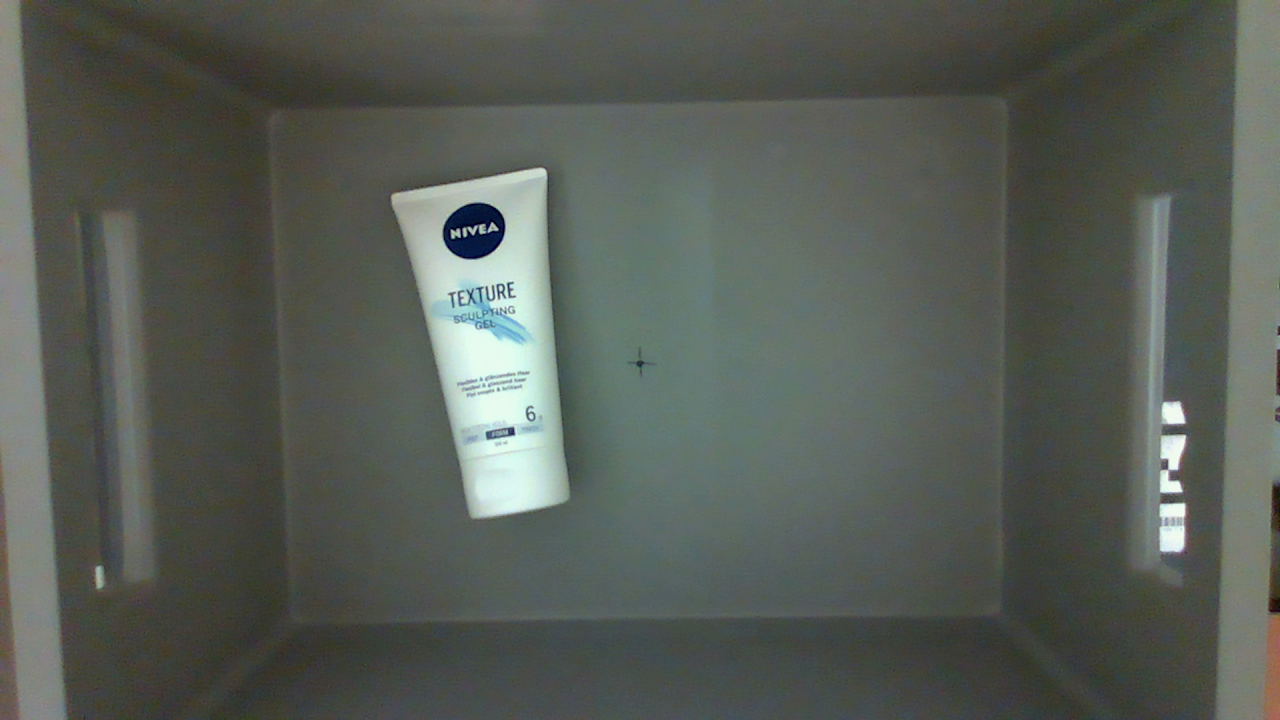
\includegraphics[width=0.5\textwidth]{graphics/methods/b0358.png}}
 \caption{The first dataset contained 4 products, with only one object in the bin}
 \label{figure: products}
\end{figure}
\clearpage
\subsection{Automatically generated dataset with multiple objects in the bin} \label{sec:multidataset}
The second dataset was made out of bottles that were available in the Robot Interaction Lab at Reykjavik University. It included 4 types of products and consists of 70 images, \textit{Alberto Balsam}(16 images), \textit{Nivea Cleansing Milk}(11 images), \textit{Nivea Elastic}(24 images) and \textit{Nivea Texture}(19 images). 
This is a robot-generated dataset with automatically generated labels, which has multiple objects in the bin. 
These objects were picked up and moved to another box. When the robot had moved the object to another bin an image was captured of the items bin in a fixed home position and added to the dataset. Then it was possible to find a difference(between before and after) and locate the object.
An example of before and after images can be seen in \textit{Figure \ref{figure: multiproducts}}. 

\begin{figure}[h]
 \centering
 % include first image
 \subfloat{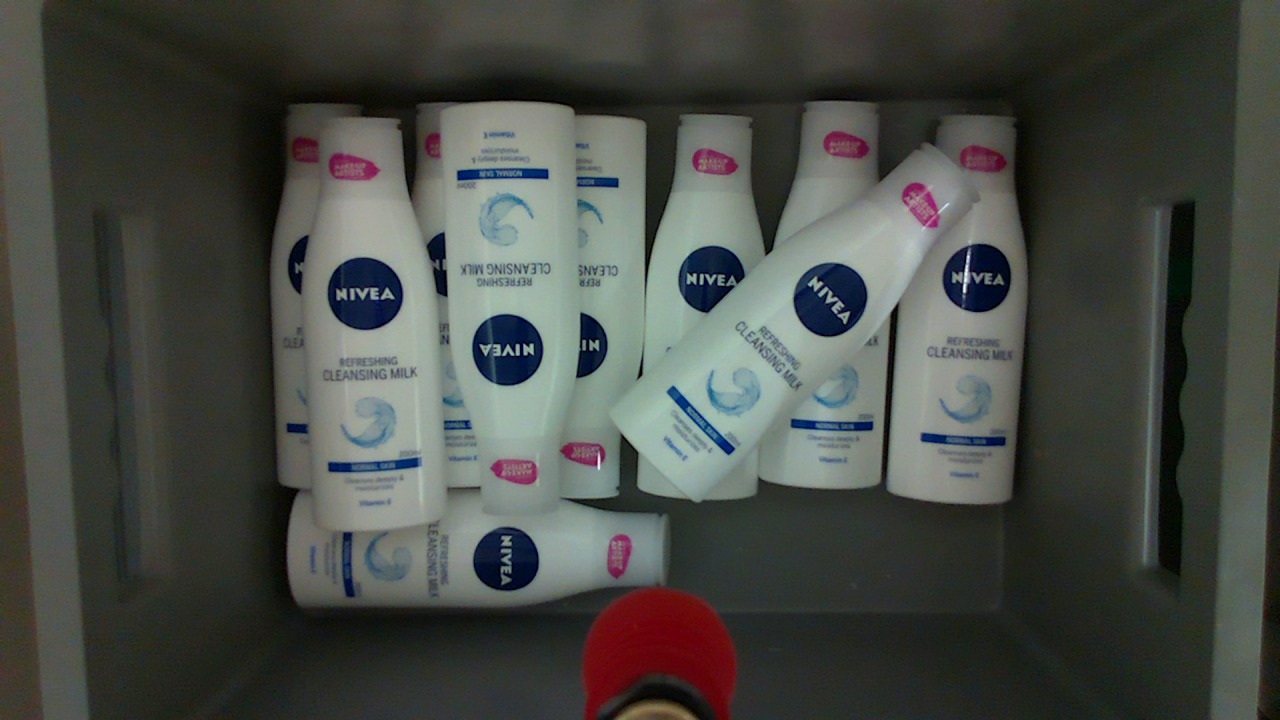
\includegraphics[width=0.45\textwidth]{graphics/results/0000.png}}
 \hfill
 %\hspace{2 cm}
 \subfloat{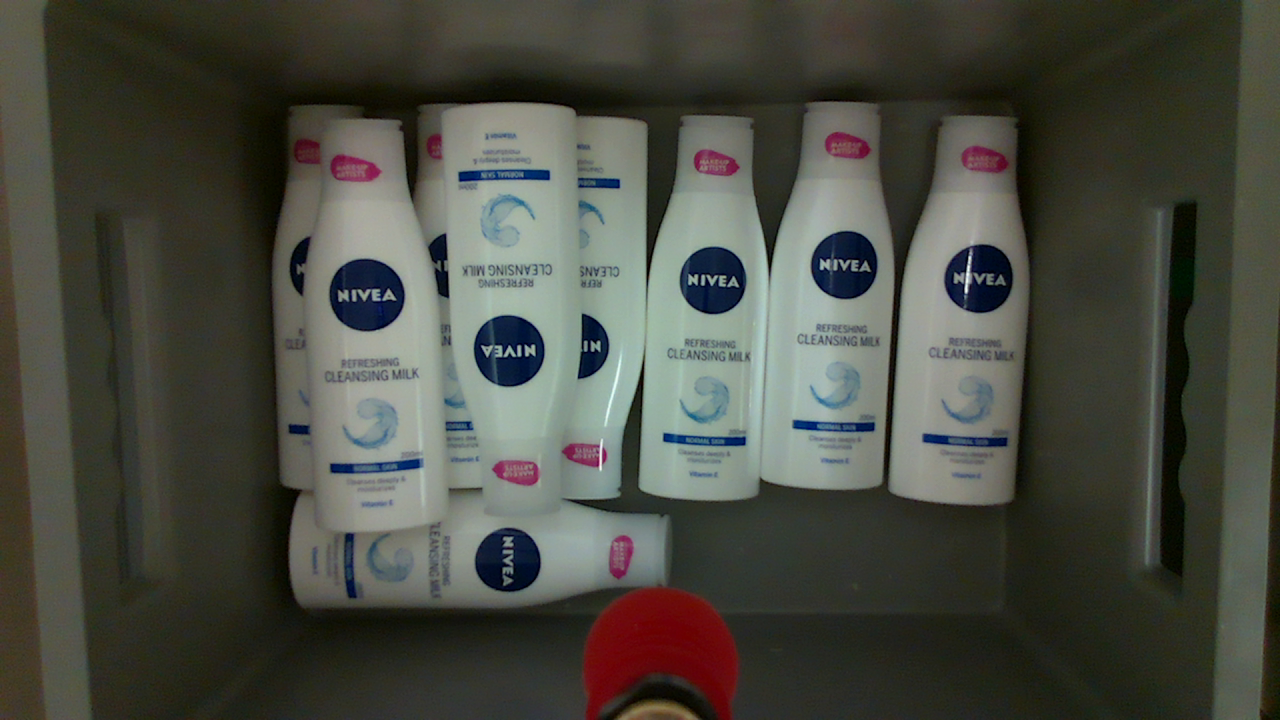
\includegraphics[width=0.45\textwidth]{graphics/results/0001.png}}
 \hfill
 %\hspace{2 cm}
 \subfloat{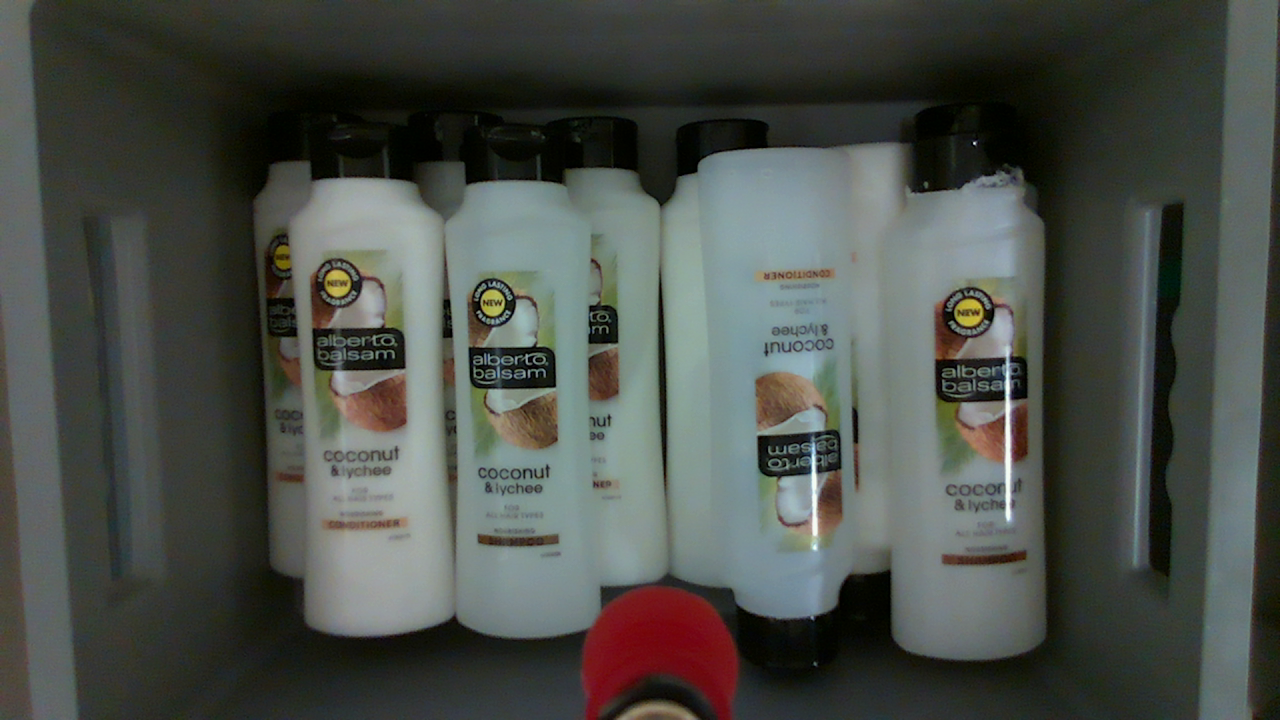
\includegraphics[width=0.45\textwidth]{graphics/results/0027.png}}
 \hfill
 %\hspace{2 cm}
 \subfloat{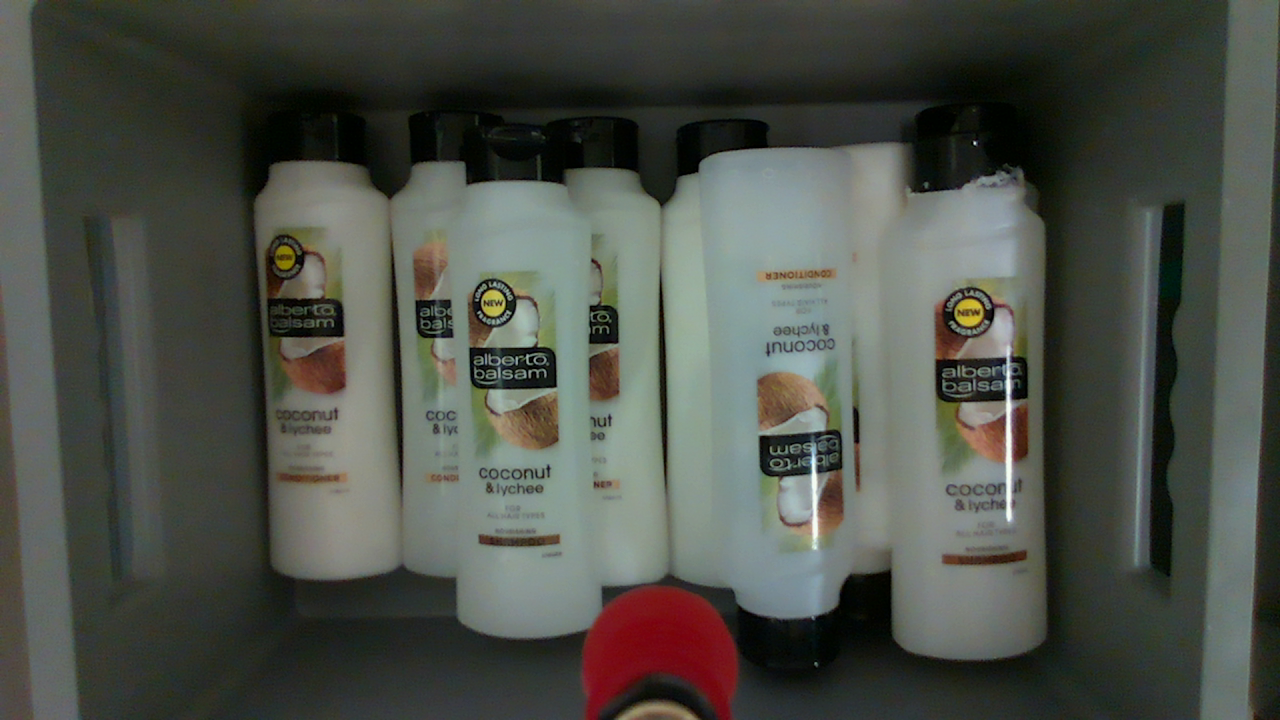
\includegraphics[width=0.45\textwidth]{graphics/results/0028.png}}
 %\hspace{2 cm}
 \hfill
 \subfloat{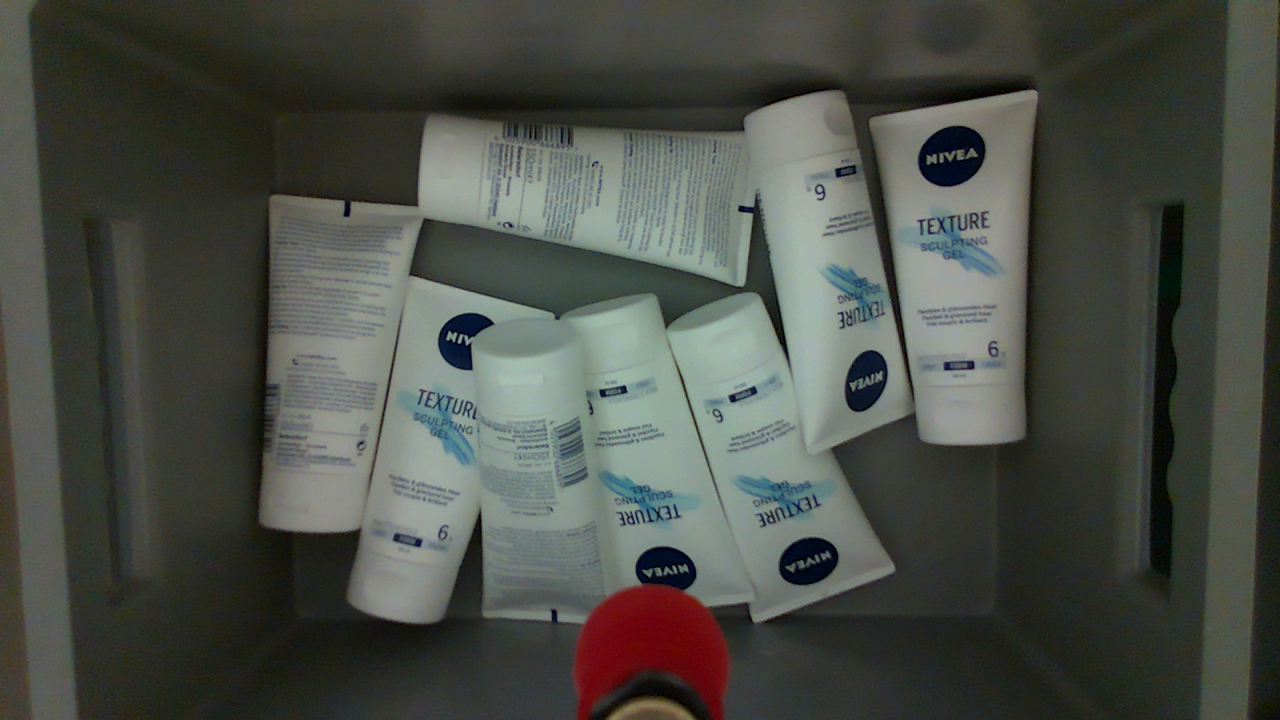
\includegraphics[width=0.45\textwidth]{graphics/results/0146.png}}
 \hfill
 %\hspace{2 cm}
 \subfloat{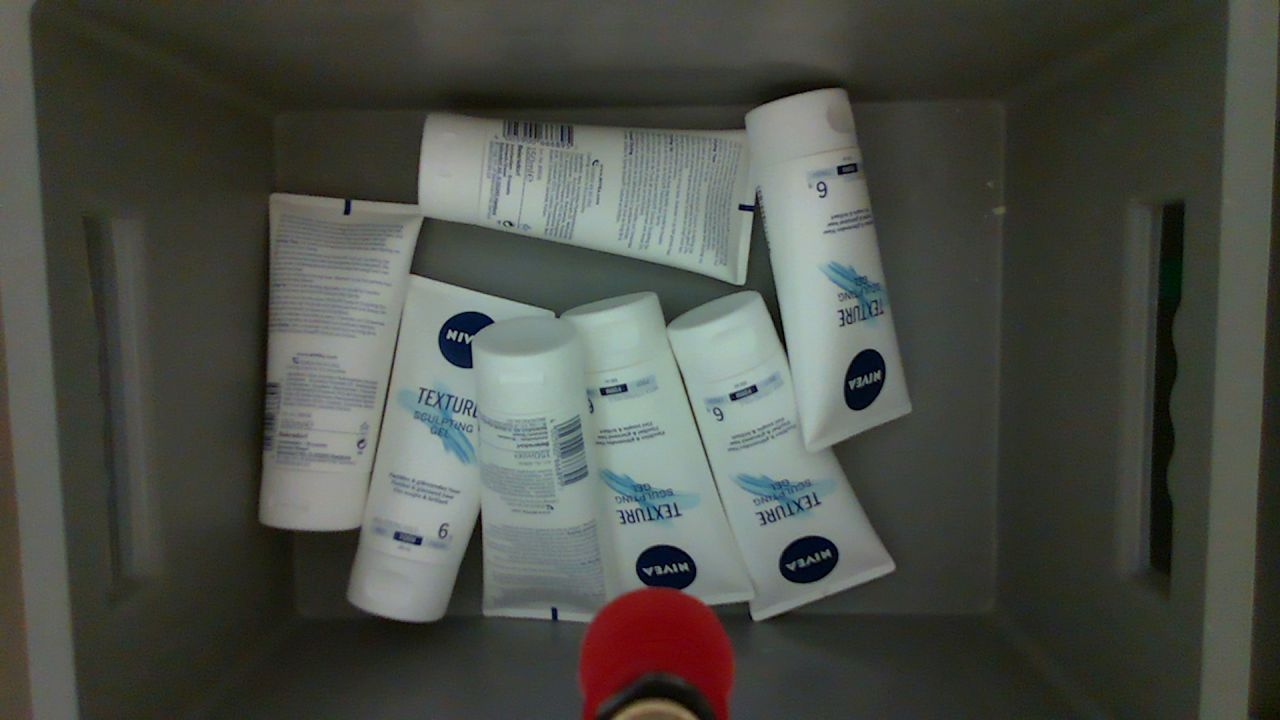
\includegraphics[width=0.45\textwidth]{graphics/results/0147.png}}
 %\hspace{2 cm}
 \hfill
 \subfloat{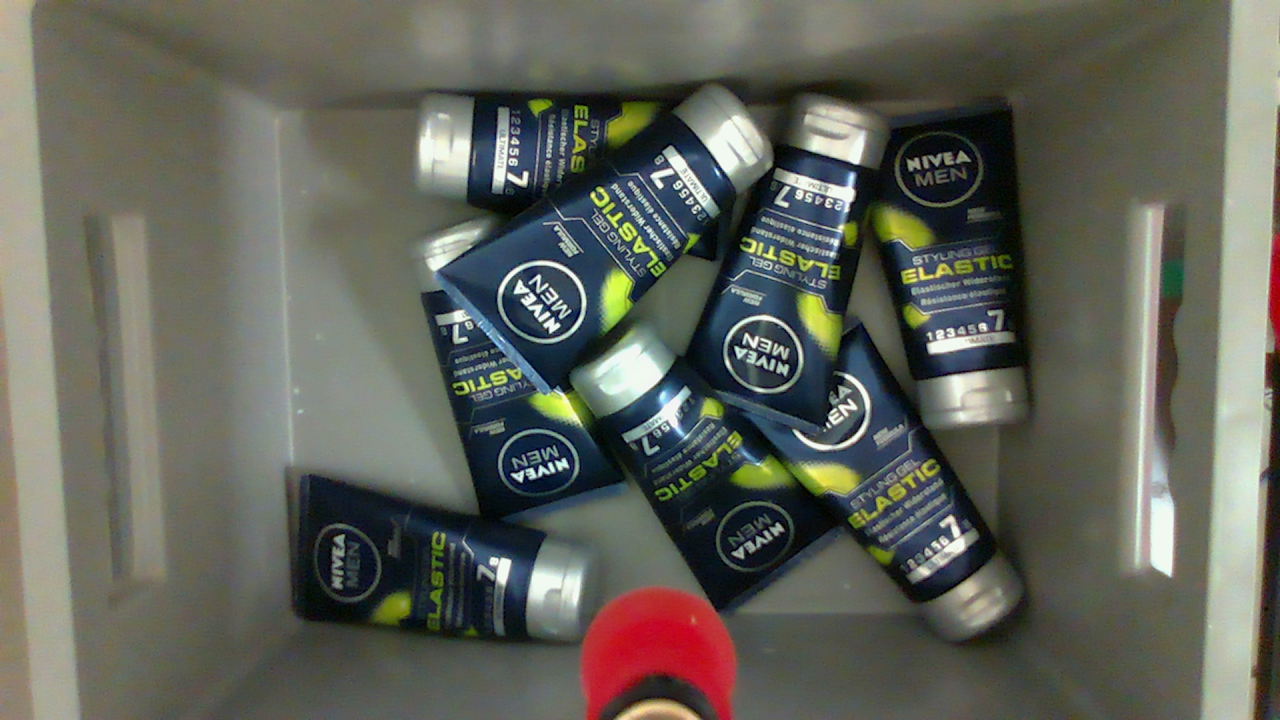
\includegraphics[width=0.45\textwidth]{graphics/results/0075.png}}
 %\hspace{2 cm}
 \hfill
 \subfloat{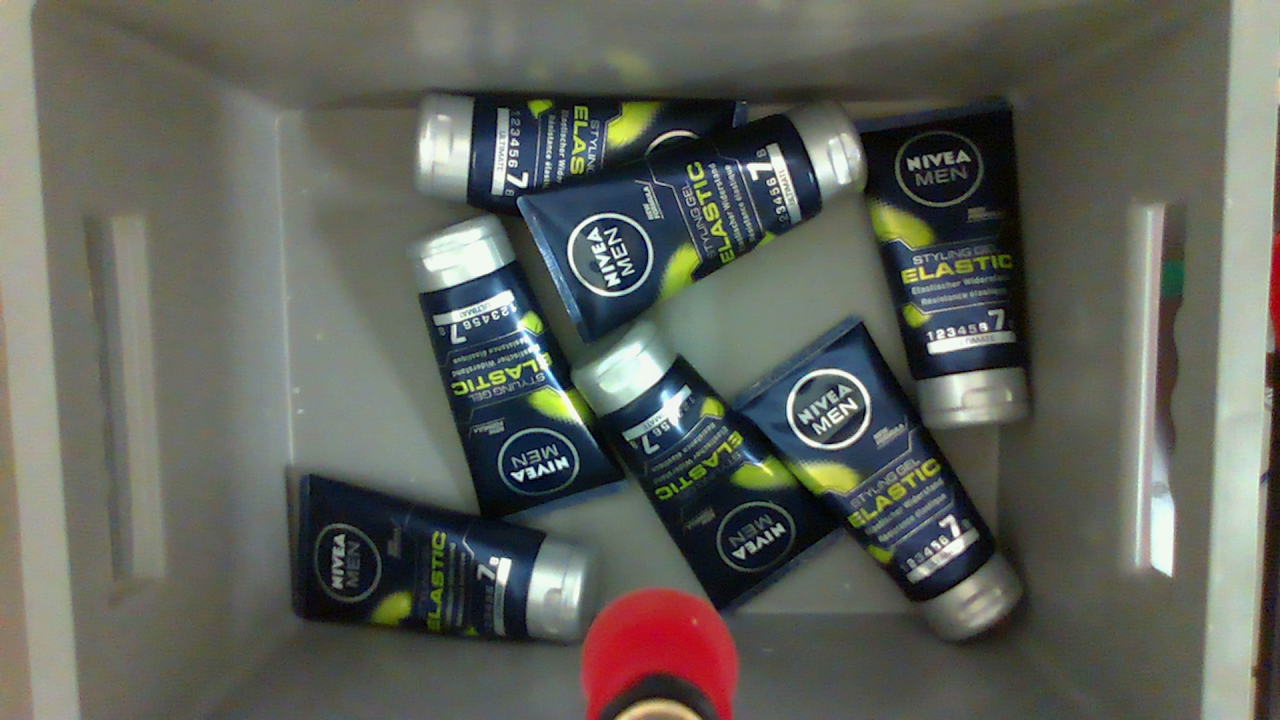
\includegraphics[width=0.45\textwidth]{graphics/results/0076.png}}
 \hfill
 
 \caption{The second dataset contained 4 products with multiple objects in the bin}
 \label{figure: multiproducts}
\end{figure}

\subsection{Beiersdorf dataset}\label{sec:beiersdorfdataset}
The Beiersdorf dataset\cite{bjarnason_detecting_2021} was used in this project as a test dataset, it was created by a former master's student in Reykjavík University. 
The dataset consists of 15 products and included 145 images per item, up to a total of 2,175 images. This dataset was diverse, with similar items and also items that have different shapes. It should therefore provide a good indication of the expected performance of a trained model in a warehouse setting, where the robot encounters previously unseen items. \textit{Figure \ref{fig:beiersdorf}} shows the items that are in the dataset.

% \begin{figure}[h]
% \centering
% 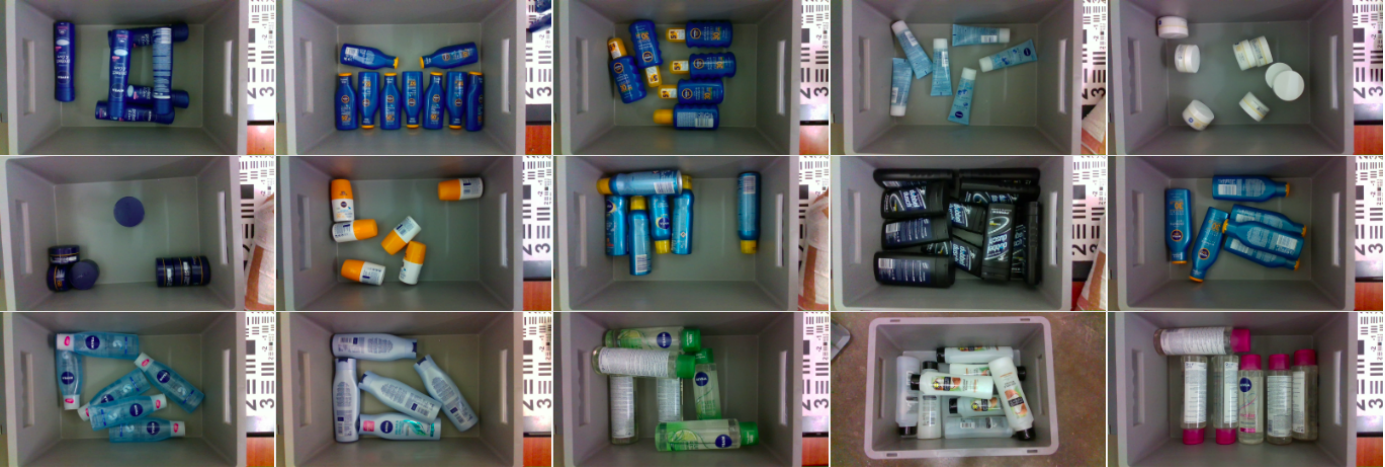
\includegraphics[width=1\textwidth]{graphics/methods/sverrirdataset.PNG}
% \caption{Beiersdorf dataset contains 15 items\cite{bjarnason_1984-_detecting_2021}}
% \label{fig:beiersdorf}
% \end{figure}

\begin{figure}[h]
 \centering
 % include first image
 \subfloat[Item 1]{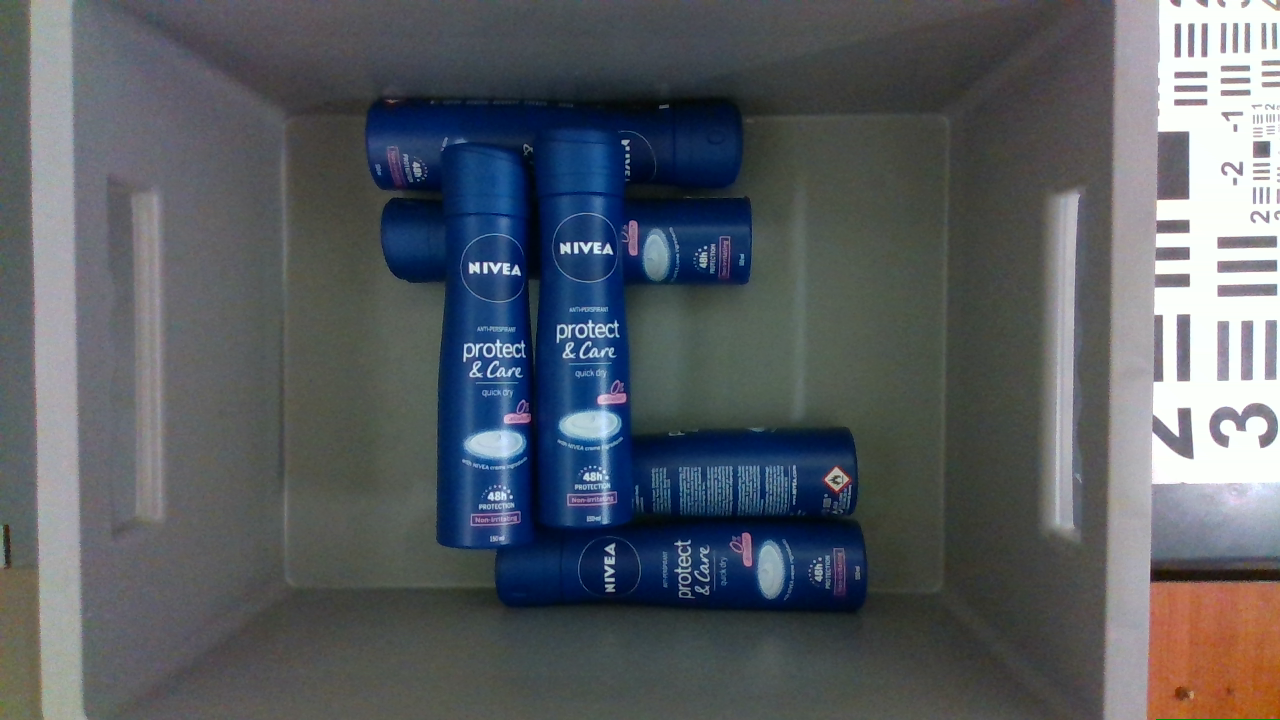
\includegraphics[width=0.2\textwidth]{graphics/beiersdorf/i0001.png}}
 \hfill
 \subfloat[Item 2]{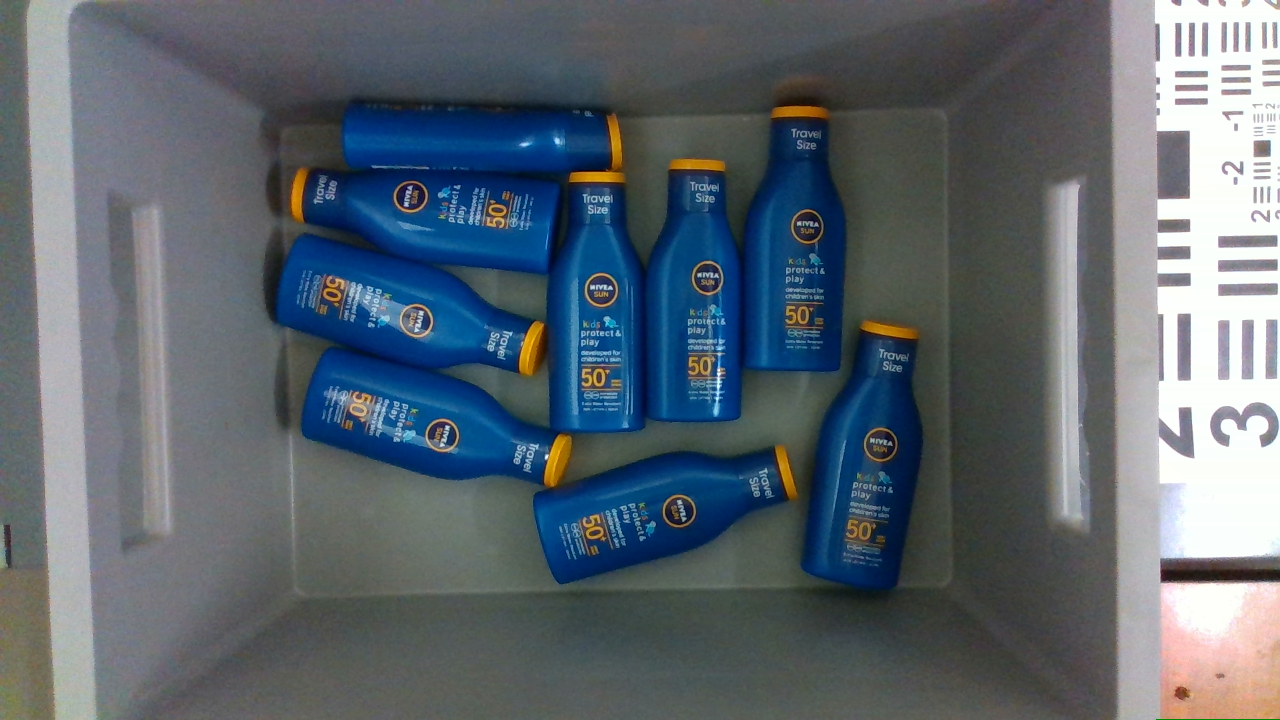
\includegraphics[width=0.2\textwidth]{graphics/beiersdorf/0155.png}}
 \hfill
 \subfloat[Item 3]{\includegraphics[width=0.2\textwidth]{graphics/beiersdorf/0300.png}}
 \hfill
 \subfloat[Item 4]{\includegraphics[width=0.2\textwidth]{graphics/beiersdorf/0450.png}}
 \hfill
 \subfloat[Item 5]{\includegraphics[width=0.2\textwidth]{graphics/beiersdorf/0650.png}}
 \hfill
 \subfloat[Item 6]{\includegraphics[width=0.2\textwidth]{graphics/beiersdorf/0750.png}}
 \hfill
 \subfloat[Item 7]{\includegraphics[width=0.2\textwidth]{graphics/beiersdorf/0950.png}}
 \hfill
 \subfloat[Item 8]{\includegraphics[width=0.2\textwidth]{graphics/beiersdorf/1050.png}}
 \hfill
 \subfloat[Item 9]{\includegraphics[width=0.2\textwidth]{graphics/beiersdorf/1250.png}}
 \hfill
 \subfloat[Item 10]{\includegraphics[width=0.2\textwidth]{graphics/beiersdorf/1350.png}}
 \hfill
 \subfloat[Item 11]{\includegraphics[width=0.2\textwidth]{graphics/beiersdorf/1470.png}}
 \hfill
 \subfloat[Item 12]{\includegraphics[width=0.2\textwidth]{graphics/beiersdorf/1650.png}}
 \hfill
 \subfloat[Item 13]{\includegraphics[width=0.2\textwidth]{graphics/beiersdorf/1750.png}}
 \hfill
 \subfloat[Item 14]{\includegraphics[width=0.2\textwidth]{graphics/beiersdorf/1950.png}}
 \hfill
 \subfloat[Item 15]{\includegraphics[width=0.2\textwidth]{graphics/beiersdorf/2050.png}}
 \caption{Beiersdorf dataset contains 15 items\cite{bjarnason_detecting_2021}}
 \label{fig:beiersdorf}
\end{figure}

The dataset includes manually annotated object masks in the form of polygons tracing the outline. For use with Yolo, bounding boxes were generated from the masks as the minimum and maximum vertex coordinate of each polygon.
It takes 2-10 minutes to annotate an image by hand, averaging approximately 5 minutes per image. When the images are 2175 it takes around 181 hours to annotate all the images. Which is a lot of manpower for annotating images. \textit{Figure \ref{fig:beiersdorfanno}} shows how the dataset was annotated with a COCO annotator\cite{brooks_jsbrokscoco-annotator_2021}.
\begin{figure}[h]
 \centering
 \includegraphics[width=1\textwidth, angle =0]{graphics/methods/sverrirannotated.PNG}
 \caption{Beiersdorf dataset annotated\cite{bjarnason_detecting_2021}}
 \label{fig:beiersdorfanno}
\end{figure}

\clearpage
%----------------
\section{Experiment setup}
A set of experiments were conducted to provide answers to the research questions. In particular i) Is it possible to generate new arrangements of objects using a robot manipulator? ii) Is it possible to annotate objects automatically, determining the extent of the objects in the images? iii) Is it possible to improve the performance of a Convolutional Neural Network using automatically generated training data from a robot? Those experiments will be explained in more detail in this section. 
\subsection{Robot performance}
In this experiment, one test was done on the Franka Emika robot and that was time performance over few iterations. In this particular test, there was only one object in the bin at a time. The time performance was tested on two items \textit{Alberto Balsam} and \textit{Nivea Cleansing Milk}, first with 100 iterations and then with 300 iterations. This gave us the movement time for one object. In addition, it was checked if the robot needed some help to pick up the item. The robot code and how it works is explained in \textit{Section \ref{robotcontrol}}. 

\subsection{Automatic labelling performance}
The automatic labelling is not simple, since you need to look at few things such as lighting conditions, light reflection from objects, shades, etc. 
%So two methods were tested that were described in the methods chapter. 
In the automatic labeling experiment, two tests were performed on two methods that were mention in \textit{Sections \ref{beforeandafter}}

One test was performed on the \textit{Before vs After}. That test was simple and was only a visual inspection executed on the output images, to see how this method would work. %affect the results.

The other test was performed on the \textit{Empty vs Item in the bin}. That test was executed by a visual inspection of the output images to check if the image has a good or bad annotation. Bad annotation is when the bounding box does not frame the object tightly, and is extremely bad when the center point is unsuitable for picking. An example of a good and bad annotation is shown in \textit{Figure \ref{figure: goodandbad}}. The time that it takes to annotate the images was also measured.

\begin{figure}[h]
 \centering
 \subfloat[Good annotation ]{\includegraphics[width=0.5\textwidth]{graphics/methods/albertobalsam100_0006box.png}}
 \hfill
 \subfloat[Bad annotation]{\includegraphics[width=0.5\textwidth]{graphics/methods/albertobalsam100_0050box.png}}
 \caption{An example of how good and bad annotations would look like}
 \label{figure: goodandbad}
\end{figure}
\clearpage

\subsection{Trained neural network performance}
%\fxfatal{Describe here or refer to the earlier description of the training setup, including network architecture (Yolov4), relevant sizes, image resolution, and implementation framework (with references). Make a special note of any relevant changes in hyperparameter values and refer to the config files in the appendix.}
The main network architecture that was used in this project was the YOLOv 4 (\textit{Section: \ref{sec:yolo}}), which is a convolutional neural network.
The images that neural networks train on, had the resolution of \textit{1280×720} and the framework subsampled the images to \textit{512x512}. The implementation framework that was used in this project was the Darknet, an open-source neural network\cite{alexey_alexeyabdarknet_2021}. The config file used in this project was the yolo-obj\_new.cfg and it can be found in the \textit{Appendix \ref{sec:config}}

%Hvernig netið var sett um að þetta var yolo 4 vísa í yolo section, með svona storar myndir, notað darknet útfærsluna og vísa í github, setja config skrár í appendix yolo-obj_new.cfg
%\fxfatal{Nefna að ég hafi þjálfað netið tvisvar með sama data seti, einu sinni þar sem ég var búinn að eyða út vondum myndum og einu sinni þar sem þær voru inni !!!}

Three neural networks were trained from automatically labelled datasets. 
The first two neural networks use almost the same dataset but were trained on the automatically generated dataset with one object in the bin. But when training the first neural network bad annotations were removed from the dataset. 
So the difference between them is one is fully automatic and the other has human intervention on bad annotations.
The third neural network was trained on the automatically generated dataset with multiple objects in the bin.

When the neural networks had been trained three tests were done on the neural networks, the IoU test, one visually, and an accuracy test(precision, recall, F1-score). These tests were made to see if the neural networks would improve. 

The first test was to measure which epochs model of the neural network would give us the best IoU on the test images. Epochs are the number of times the training set has been presented to the network.

The second test was done by comparing visually before and after results on the neural network, to find out if the trained neural network was performs better than the original network on trained objects in a bin. 

The third test was measuring the accuracy of object detection using a deep neural network trained on the robot-generated data. Measuring the IoU, recall, precision, and F-score and compare it to the results of manual labeling. 


\subsubsection{First neural network}
Before training the first neural network model using the \textit{automatically generated dataset with one object in the bin} (\textit{Sec:\ref{sec:firstdataset}}), it was split into a 75\% train dataset and 25\% test dataset. Images that had bad annotations were removed from the dataset. \textit{Figure \ref{fig:firstneural}} shows how the third neural network was trained.

\begin{figure}[h]
 \centering
 \includegraphics[width=0.6\textwidth]{graphics/results/firstneural.pdf}
 \caption{How the first neural network was setup}
 \label{fig:firstneural}
\end{figure}

\subsubsection{Second neural network}
The second neural network was trained as the first neural network but, the difference was the second neural network was trained on all of the automatically generated datasets with one object in the bin (\textit{Sec:\ref{sec:firstdataset}}). Before training the second neural network model using the \textit{automatically generated dataset with one object in the bin} it was split into a 75\% train dataset and 25\% test dataset, which had both bad annotations and good annotations. \textit{Figure \ref{fig:secondneural}} shows how the third neural network was trained.


\begin{figure}[h]
 \centering
 \includegraphics[width=0.6\textwidth]{graphics/results/secondneural.pdf}
 \caption{How the second neural network was setup}
 \label{fig:secondneural}
\end{figure}

\subsubsection{Third neural network}
The third neural network was trained on the automatically generated dataset with multiple objects in the bin (\textit{Sec:\ref{sec:multidataset}}) and on the automatically generated dataset with one object in the bin(\textit{Sec:\ref{sec:firstdataset}}). Both the \textit{automatically generated dataset with one object in the bin} and the \textit{automatically generated dataset with multiple objects in the bin} were split into a 75\% train dataset and 25\% test dataset before training the third neural network. \textit{Figure \ref{fig:thirdneural}} shows how the third neural network was trained.

\begin{figure}[h]
 \centering
 \includegraphics[width=0.6\textwidth]{graphics/results/thirdneural.pdf}
 \caption{How the third neural network was setup}
 \label{fig:thirdneural}
\end{figure}